\newcount\draft\draft=1 % set to 0 for submission or publication
\documentclass[phd,tocprelim]{cornell}
%
% tocprelim option must be included to put the roman numeral pages in the
% table of contents
%
% The cornellheadings option will make headings completely consistent with
% guidelines.
%
% This sample document was originally provided by Blake Jacquot, and
% fixed up by Andrew Myers.
%
%Some possible packages to include
\usepackage{graphics}
\usepackage{moreverb}
%\usepackage{subfigure}
\usepackage{epsfig}
\usepackage{hangcaption}
\usepackage{newtxtext}
\usepackage{newtxmath}
\usepackage{palatino}

% Gator cruft
\let\openbox\relax
\usepackage{amsmath}
\usepackage{amsthm}
\usepackage{bbm}
\usepackage{amsfonts}
\usepackage{syntax}
\usepackage{tikz}
\usetikzlibrary{decorations.pathmorphing}
\usepackage{url}
\usepackage{graphicx,pstricks}
\usepackage{xspace}
\usepackage{xxx}
\usepackage{proof}
\usepackage{listings}

\lstset{escapeinside={<@}{@>}} % for color _coding_
\usepackage{booktabs} % for professional tables
\usepackage{subcaption}
\usepackage{bm}

\usetikzlibrary{shapes,arrows, chains}
\usepackage[ligature, inference]{semantic}
\usepackage[T1]{fontenc}
\usepackage{mathpartir}
\usepackage{nccmath}

\newcommand{\mat}{\mathsf{mat}_{n_1{\times}n_2}}
\newcommand{\env}[1]{#1,\sigma}
\newcommand{\defas}{\mathrel{::=}}
\newenvironment{leftalign}%
{\fleqn[5pt]\csname align*\endcsname}%
{\csname endalign*\endcsname\endfleqn}
\newcommand{\alt}{\:|\:}
\newcommand{\bmark}{\textsf}

\mathlig{->}{\rightarrow}
\mathlig{|-}{\vdash}
\mathlig{=>}{\Rightarrow}

% Commutativity Stuff
\usepackage{algorithm2e}
\usepackage{microtype}
\usepackage{fncylab}
\usepackage{float}
\usepackage{balance}
%

\labelformat{algocf}{Algorithm~#1}

\tikzstyle{block} = [rectangle, draw, fill=gray!20,
text width=4em, text centered, rounded corners, minimum height=4em]
\tikzstyle{line} = [draw, -latex']

% Code listings configuration.
\lstdefinelanguage{GLSL}{
	keywords={void, float, int, with, auto,
		if, abs, \#ifdef, \#else, \#endif, in, out, uniform,
		varying, attribute, return, void, space, is, coord, canon, type,
		declare, vec, mat, as, has, frame, object, dimension, coord},
	comment=[l]{//},
}
\lstset{
	language=GLSL,
	columns=fullflexible,
	keepspaces=true,
	showspaces=false,
	showstringspaces=false,
	keywordstyle=\bfseries,
	basicstyle=\ttfamily\small,
	basewidth=0.53em,
	aboveskip=0.9\medskipamount,
	belowskip=0.6\medskipamount,
	mathescape=true,
	lineskip={-2pt},
	commentstyle=\color{gray},
	% xleftmargin=\parindent,
}

% Shorthand for inline code.
\newcommand{\code}{\lstinline[keywordstyle=]}

% color definitions
\definecolor{darkolivegreen}{rgb}{0.33, 0.42, 0.18}

% Semantics declarations for the formalism.
\DeclareRobustCommand\tvdash{\mathrel{||}\joinrel\mkern-.5mu\mathrel{-}}
\newcommand{\source}[1]{\llbracket #1 \rrbracket}
\newcommand{\ld}[1]{\leq_\Delta}
\newcommand{\gen}[1]{\langle #1 \rangle} %generic
\newcommand{\sca}[0]{\textrm{scalar}}
\newcommand{\subsumption}{\textrm{SUBSUMPTION}}
\newcommand{\unit}{\textrm{UNIT}}
\newcommand{\scalar}{\textrm{SCALAR}}
\newcommand{\vect}{\textrm{VECTOR}} %both vec and vector lead to funky behavior
\newcommand{\matr}{\textrm{MATRIX}} %can't call this matrix because amsmath
\newcommand{\decl}{\textrm{DECL}}
\newcommand{\assign}{\textrm{ASSIGN}}
\newcommand{\add}{\textrm{ADDITION}}
\newcommand{\smul}{\textrm{SCAL MUL}}
\newcommand{\vmul}{\textrm{VEC MUL}}
\newcommand{\mmul}{\textrm{MAT MUL}}
\newcommand{\vcmul}{\textrm{VEC CMUL}}
\newcommand{\mcmul}{\textrm{MAT CMUL}}

\newcommand{\IH}{\textrm{I.H.}}
\newcommand{\TC}{\textrm{T.C.}}
\newcommand{\sub}{\textrm{SUBST}}

\newif\ifsemanticsdoc

\newtheorem{lemma}{Lemma}
\newtheorem{theorem}{Theorem}

%if you're having problems with overfull boxes, you may need to increase
%the tolerance to 9999
\tolerance=9999

\bibliographystyle{plain}
%\bibliographystyle{IEEEbib}

\renewcommand{\caption}[1]{\singlespacing\hangcaption{#1}\normalspacing}
\renewcommand{\topfraction}{0.85}
\renewcommand{\textfraction}{0.1}
\renewcommand{\floatpagefraction}{0.75}

\title {Language Designs for Geometry and Heterogeneous Reasoning in Graphics Programming}
\author {Dietrich Geisler}
\conferraldate {August}{2024}
\degreefield {Ph.D.}
\copyrightholder{Dietrich Geisler}
\copyrightyear{2024}

\begin{document}

\maketitle
\makecopyright

% Enable our \mathlig substitutions.
\mathligson

\begin{abstract}
\xxx[dg]{TODO: fix up?}
There has been growing demand for 3D image rendering in the past several decades, primarily from video games, but also from fields as broad as film, art, architecture, and scientific simulation.  A major challenge with expanding use of rendering, however, is that the programming is difficult, requiring significant field expertise when abstractions break down.

In this dissertation, we will examine how we may be able to design programming languages to ameliorate some of these challenges.  Our goal will be to examine two specific challenges in graphics programming reasoning: geometric correctness and performance in heterogeneous device communication.  

In the first part of this talk, we will discuss Gator, a language which provides type-level reasoning for a class of bugs we describe as "geometry bugs", as well as a lightweight mechanism to reason about operations on geometry.  In the second part of this talk, we will discuss Caiman, a language which typechecks heterogeneous implementations against a fixed specification.  We will also examine how Caiman's type-level restrictions allow for separating performance and correctness, as well as providing a mechanism for restricted synthesis of heterogeneous programs.
\end{abstract}

\begin{biosketch}
Your biosketch goes here. Make sure it sits inside
the brackets.
\end{biosketch}

\begin{dedication}
This document is dedicated to all Cornell graduate students.
\end{dedication}

\begin{acknowledgements}
Your acknowledgements go here. Make sure it sits inside the brackets.
\end{acknowledgements}

\contentspage
\tablelistpage
\figurelistpage

\normalspacing \setcounter{page}{1} \pagenumbering{arabic}
\pagestyle{cornell} \addtolength{\parskip}{0.5\baselineskip}

\chapter{Introduction}

\xxx[dg]{As a blanket note, I'll add references to this section later}

Computer graphics has long been a core field of study within computer science.  In the past decade alone, computer graphics has seen application in video games, animated film, scientific simulation, data visualization, and medical devices.  The term computer graphics itself has become so broad as to be fuzzy; we refer here specifically to the study of modeling and rendering snapshots of 2 or 3-dimensional spaces onto a screen.

Despite the number of applications and domains that make use of computer graphics, maintaining or using software systems for rendering (such as a \emph{rendering engine}) can be extremely difficult and time--consuming.  Manipulating a rendering engine can require specialized learning in topics as diverse as light physics, geometry, visual design, and material science.  Additionally, the history of these specialized topics can often find themselves at odds with the practical realities of building a performant computer system, resulting in complex engineering constraints and implicit rules for manipulating code.

As a consequence of this complexity, computer graphics has many domain--specific challenges that have been solved through sheer engineering prowess and, to put it bluntly, hacks on the tools available.  For instance, game engines are frequently specialized to C++ engineering, relying on macros to control performance characteristics and providing highly specialized program behavior.  Similarly GPUs come equipped with a rendering pipeline originally meant for the usual case of computer graphics, but as programmer specialization has outpaced hardware design, the GPU rendering pipeline has been taken apart and pieced back together to squeeze more performance or a specific behavior out of this hardware.

These challenges in graphics programming have real cost: large--scale rendering engines can be difficult to update for new technologies (such as Unreal Engine lumbering towards supporting raytracing), non--experts can be forced to rely on black--box implementations without any realistic mechanism to customize these implementations, and performance can be left on the table in critical applications (there are some interesting examples of this, I need to find ``good references" though).

The sheer breadth and complexity of these computer graphics and rendering systems, however, poses a unique opportunity for programming language designers.  Improvements in languages for graphics specifically could provide mechanisms that keep up with graphics programmer needs faster than hardware design, and can expose domain--specific design challenges with interesting consequences for language research as a whole (I have a couple of citations here related to sampling theory).

Despite there being both potential and real need for graphics--specific programming language design, this focus of study has remained largely untapped.  Notable efforts in this direction include languages for static and dynamic reasoning about the rendering pipeline and specialized languages for automatic and symbolic differentiation in geometric spaces.  There are, however, few other high--profile efforts, despite anecdotally there remaining many potentially interesting problems (which will be further discussed in Section~\ref{subsec:problems}).

\subsection{Summary of Work}

In this dissertation, we present work that both identifies and provides language--level solutions for two specific challenges in graphics programming: geometric reasoning and performance exploration.  In both cases, we identify properties of graphics programs which are either stated informally or otherwise known to the programmer, but are not communicated to the typechecker and compiler.  Without this necessary context for the intended program semantics, the programmer loses the benefits of static typechecking and compiler optimizations, and may be forced to introduce the various C++ hacks described earlier.

Concretely, we describe three pieces of work:
%
\begin{itemize}
\item Gator, a language for providing semantics and typechecking for graphics--style geometry
\item A paper on commutative diagram verification needed to solve a technical problem within Gator
\item Caiman, a language for providing type--level support for heterogeneous performance exploration
\end{itemize}
%
Both Gator and the commutative diagram paper have been previously published.

Chapter 2 explores the relationship between the geometry of a scene being rendered and the code used to calculate properties of that scene through the lens of the Gator language.  By identifying and naming three commonly--needed pieces of geometric information, Gator is able to provide geometry-aware types and semantics for several core graphics algorithms.  We also show how introducing these types enables the Gator compiler to safely synthesize light--weight geometric transformations.  The guarantees Gator aims to provide, however, resulted in needing a solution for online verification of commutative diagrams, a technical layer described further in Chapter 3.

Chapter 4 changes our focus to the performance concerns of graphics programmers, and specifically the narrow problem of inter--device communication, or heterogeneous programming.  We introduce a language, Caiman, which provides a type system and compiler implementation for separating semantic and performance concerns in heterogeneous settings.  We additionally develop and implement an algorithm for synthesizing these (otherwise complex) transformations in a type--directed and decomposable way, allowing a programmer to explore performance characteristics of a compiled program while maintaining control over the details of that program.

\subsection{Open Directions}
\label{subsec:problems}

I plan to think about this section more, I'll defer on writing it for now.

\chapter{Gator: Geometry Types for Graphics Programming}

%\documentclass[../main.tex]{subfiles}

\section{Introduction}
\label{sec:intro}

Applications across a broad swath of domains use linear algebra to represent geometry, coordinates, and simulations of the physical world.
Scientific computing workloads, robotics control software, and real-time graphics renderers all use matrices and vectors pervasively to manipulate points according to linear-algebraic laws.
The programming languages that express these computations, however, rarely capture the underlying \emph{geometric} properties of these operations.
In domains where performance is critical, most languages provide only thin abstractions over the low-level vector and matrix data types that the underlying hardware (i.e., GPU) implements.
A typical language might have a basic \code{vec2} data type for vectors consisting of two floating-point numbers, for example, but not distinguish between 2D vectors in rectangular or polar coordinates---or between points in differently scaled rectangular coordinate systems.

This paper focuses on real-time 3D rendering on GPUs, where correctness hazards in linear algebra code are particularly pervasive.
The central problem is that graphics code frequently entangles application logic with abstract geometric reasoning. Programs must juggle vectors from a multitude of distinct coordinate systems while simultaneously optimizing for performance.
This conflation of abstraction and implementation concerns makes it easy to confuse different coordinate system representations and to introduce subtle bugs.
Figure~\ref{fig:bunnyimages} shows an example: a coordinate system handling bug yields incorrect visual output that would be difficult to catch with testing.

\subsection{The Problem}

\begin{figure}
\begin{minipage}{.48\linewidth}
\centering
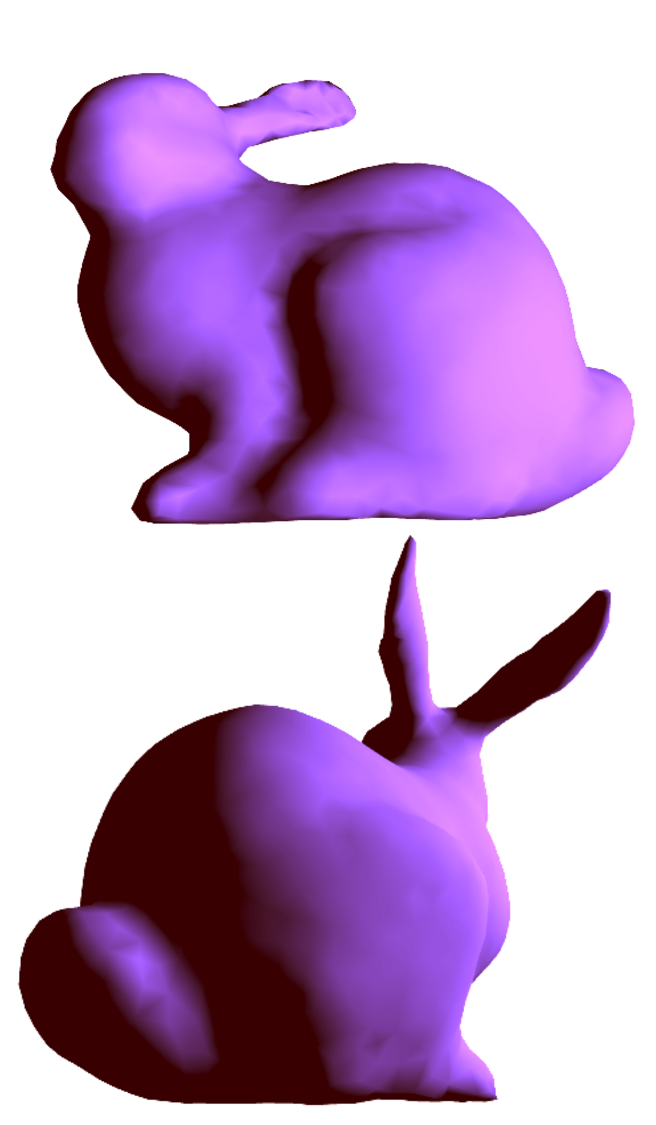
\includegraphics[scale=0.25]{fig/goodbunnies.pdf}
\caption{Correct implementation.}
\label{fig:bunnygood}
\end{minipage}
\begin{minipage}{.48\linewidth}
	\centering
	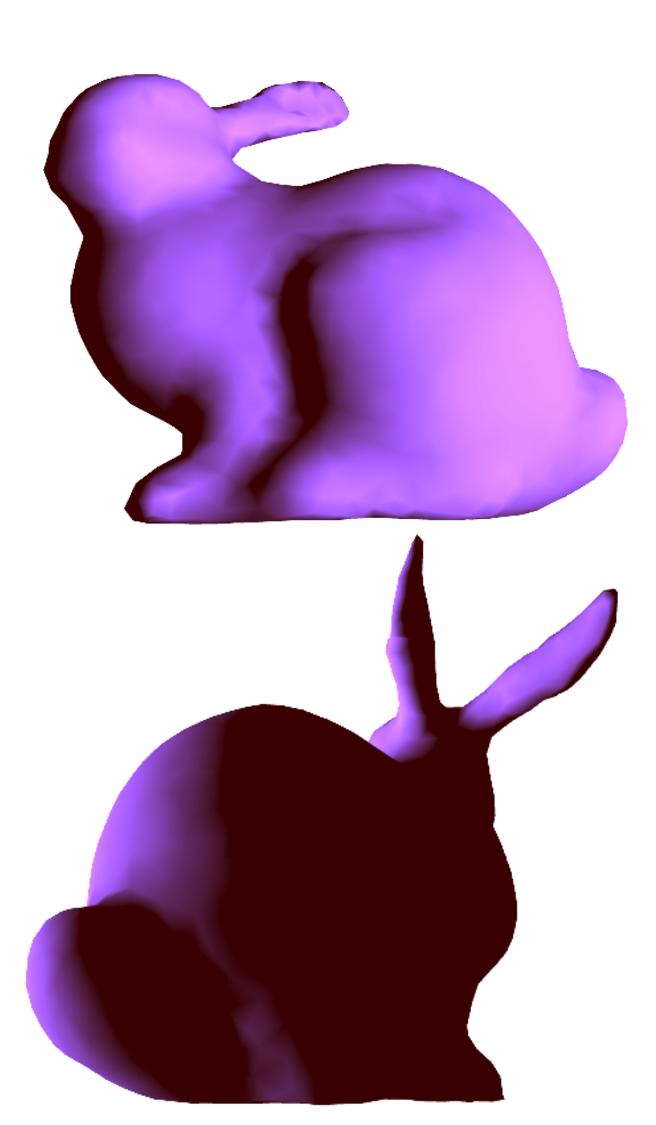
\includegraphics[scale=0.25]{fig/badbunnies.pdf}
	\caption{Incorrect implementation.}
	\label{fig:bunnybad}
\end{minipage}
\caption{Objects rendered with an implementation of the diffuse component of Phong lighting~\cite{phong},
% where the light source is fixed to the top right of the screen,
without (a) and with (b) a coordinate system transformation bug.
The root cause is an incorrect spatial translation of the light source.
The problem is only visible from one side of the model.}
\end{figure}
\begin{figure}
\centering
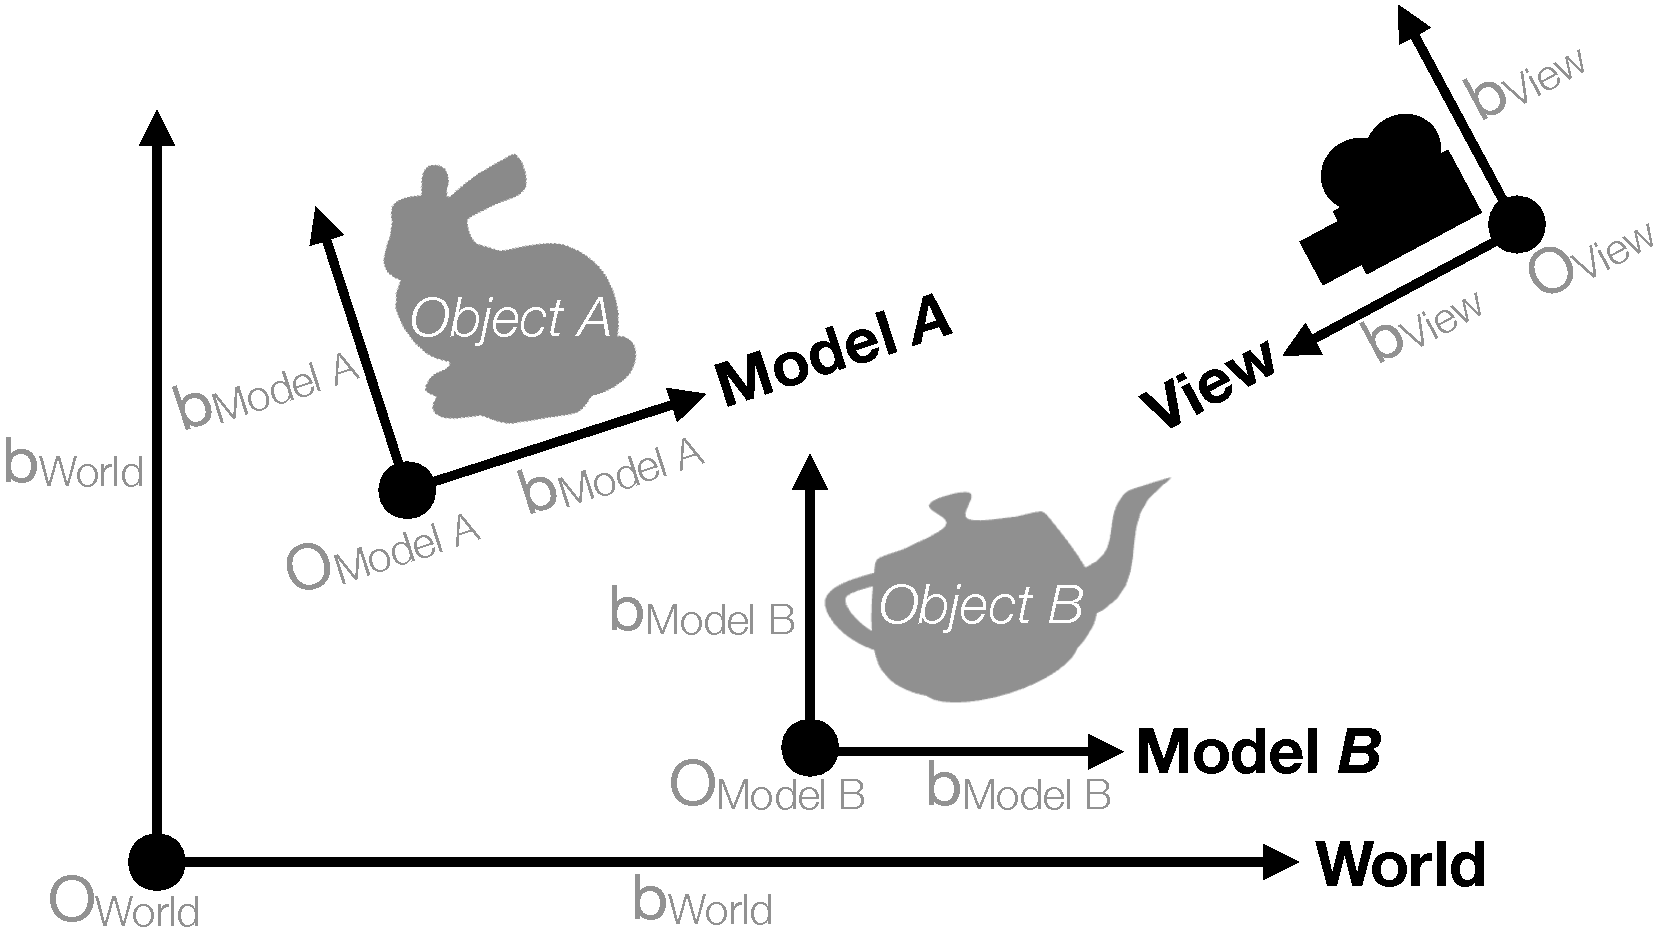
\includegraphics[width=\linewidth]{fig/coordinate-spaces-2.pdf}
\caption{Coordinate systems in graphics code.
	\textbf{Model A}, \textbf{Model B}, \textbf{World}, and \textbf{View} are coordinate systems.
	A coordinate system is defined by its basis vectors $b$ and origin $O$.
	% Ridiculous LaTeX note: the underscores in $b_s$ and $O_s$ were causing labeling issues. I reworded this to just refer to $b$ and $O$ by themselves to avoid this. I think it reads clearly enough this way. --A
	The \textbf{View} represents the perspective of a simulated camera.
	% Deleted the below because it doesn't seem 100% relevant.
	% Applications perform geometric operations on objects in either world or view space, depending on whether these operations require information about the viewer.
}
\label{fig:spaces}
\end{figure}

Coordinate systems proliferate in graphics programming because 3D scenes consist of many individual objects.
Figure~\ref{fig:spaces} depicts a standard setup for rendering two objects in a single scene.
Each object comes specified as a \emph{mesh}, which consists of coordinate vectors for each vertex position.
The mesh provides these vectors in a local, object-specific coordinate system called \emph{model} space.
The application positions multiple objects relative to one another in \emph{world} space,
and the simulated camera's position and angle define a \emph{view} space.

Renderer code needs to combine vectors from different coordinate systems, such as in this distance calculation:
%
\begin{lstlisting}
float dist = length(teapotVertex - bunnyVertex);
\end{lstlisting}
%
This code may be incorrect, however, depending on the representation of the \code{teapotVertex} and \code{bunnyVertex} vectors.
If the values come from the mesh data, they are each represented in their respective model spaces---and subtracting them yields a geometrically meaningless result.
A correct computation needs to convert the operands into a common coordinate system using \emph{affine transformation} matrices:
%
\begin{lstlisting}
float dist = length(teapotToWorld * teapotVertex - 
	bunnyToWorld * bunnyVertex);
\end{lstlisting}
%
Here, the \code{teapotToWorld} and \code{bunnyToWorld} matrices define the transformations from each model space into world space.

\paragraph{Geometry bugs are hard to catch.}

Mainstream rendering languages like OpenGL's GLSL~\cite{opengl} cannot statically rule out coordinate system mismatches.
In GLSL, the variables \code{teapotVertex} and \code{bunnyVertex} would both have the type \code{vec3}, i.e., a tuple of three floating-point numbers.
%
These bugs are also hard to detect dynamically.
They do not crash programs---they only manifest in visual blemishes.
While the buggy output in Figure~\ref{fig:bunnybad} clearly differs from the correct output in Figure~\ref{fig:bunnygood}, it can be unclear what has gone wrong---or, when examining the buggy output alone, that anything has gone wrong at all.
Accordingly, writing assertions or unit tests to catch this kind of bug can be challenging: specifying the behavior of a graphics program requires formalizing how the resulting scene should be perceived.
Viewers can perceive many possible outputs as visually indistinguishable, so even an informal specification of what makes a renderer ``correct,'' for documentation or testing, can be difficult to write.

\paragraph{Geometry bugs in the wild.}

Even among established graphics libraries, geometry bugs can remain latent until a seemingly correct API change reveals the bug.
% For example, in LÖVR, a framework for rapidly building VR experiences, the developers discovered a bug where a variable that was in one space was being used as if it was in another.\footnote{\url{https://github.com/bjornbytes/lovr/issues/55}}
This bug lay dormant while, to quote one of the maintainers, ``there was a change in the rendering method that amplified the problems caused by this.'' The maintainer then noted that they needed to ``go backfill this fix to all the docs/examples that have the broken version.''
Because their effects are hard to detect, geometry bugs can persist and cause subtle inaccuracies that grow as code evolves.

We found similar issues that arise when APIs fail to specify information about vector spaces.
% In the Processing graphical IDE, for example, confusion surrounding a camera API led to a 20-comment thread before a developer concluded that ``better documentation could alleviate this to some extent: it needs to be clear that modelspace is relative to the camera at the time of construction.''\footnote{\url{https://github.com/processing/processing/issues/187}}
% And in the visualization library GLVisualize.jl, users disagree about the space that the library uses for a light position.\footnote{\url{https://github.com/JuliaGL/GLVisualize.jl/pull/188}}
The root cause in both cases is that the programming language affords no opportunity to convey vector space information.

This paper advocates for making geometric spaces manifest in programs themselves via a type system.
Language support for geometric spaces can remove ambiguity and provide self-documenting interfaces between parts of a program.
Static type checking can automatically enforce preconditions on geometric operations that would otherwise be left unchecked.


\subsection{Geometry Types}

We introduce a type system that can eliminate this class of bugs, and we describe a mechanism for automatic transformation that can rule out some of them by construction.
\emph{Geometry types} describe the coordinate system representing each value and the transformations that manipulate them.
A geometry type encodes three components:
the \emph{reference frame}, such as model, world, or view space;
the \emph{geometric object}, such as a point or a direction;
and the \emph{coordinate scheme}, such as Cartesian or spherical coordinates.
Together, these components define which geometric operations are legal and how to implement them.

The core contribution of this paper is that all three components of geometry types are necessary.  
The three aspects interact in subtle ways, and real-world graphics rendering code varies in each component.
Simpler systems that only use a single label~\cite{safegi} cannot express the full flexibility of realistic rendering code and cannot cleanly support automatic transformations.
We show how encoding geometry types in a real system can help avoid and eliminate realistic geometry bugs.
We will explore further how these components are defined and interact to provide operation information in Section~\ref{sec:langlang}.

We design a language, Gator, that builds on geometry types to rule out coordinate system bugs and to automatically generate correct transformation code.
In Gator, programmers can write \code{teapotVertex in world} to obtain a representation of the \code{teapotVertex} vector in the \code{world} reference frame.
% The Gator compiler finds the appropriate sequence of matrix--vector multiplications necessary to produce a result of the correct type.
The end result is a higher-level programming model that lets programmers focus on the geometric semantics of their programs without sacrificing efficiency.

We implement Gator as an overlay on GLSL~\cite{glsl}, a popular language for implementing shaders in real-time graphics pipelines.
Most GLSL programs are also valid in Gator, so programmers can easily port existing code and incrementally add typing annotations to improve its safety.
We formalize a geometry type system and show that erasing these types preserves soundness.
In our evaluation, we port rendering programs from GLSL to qualitatively explore Gator's expressiveness and its ability to rule out geometry bugs.
We also quantitatively compare the applications to standard GLSL implementations and find that Gator's automatic generation of transformation code does not yield meaningfully slower rendering time than hand-tuned (and unsafe) GLSL code.

This paper's contributions are:
%
\begin{itemize}
\item We identify a class of geometry bugs that exist in geometry-heavy, linear-algebra-centric code such as physical simulations and graphics renderers.
\item We design a type system to describe latent coordinate systems present in linear algebra computations and prevents geometry bugs.
\item We introduce a language construct that builds on the type system to automatically generate transformation code that is type correct by construction.
\item We implement the type system and automatic transformation feature in Gator, an overlay on the GLSL language that powers all OpenGL-based 3D rendering.
\item We experiment with case studies in the form of real graphics rendering code to show how Gator can express common patterns and prevent bugs with minimal performance overhead.
\end{itemize}
%
We begin with some background via a running example
before describing Gator in detail.


\section{Running Example: Diffuse Shading}
\label{sec:example}

This section introduces the concept of geometry bugs via an example:
we implement \emph{diffuse lighting}, a component of the classic Phong lighting model~\cite{phong}.\footnote{Appendix A gives a complete GLSL implementation of the Phong model.}
We assume some basic linear algebra concepts but no background in graphics or rendering.

\subsection{Gentle Introduction to Shader Programming}
Shader programs are code, typically written in C-like languages such as GLSL or HLSL, that runs on the GPU to render a graphics \emph{scene}. The GPU executes a pipeline of shader programs, where each shader is specialized to transform a certain property of a graphical object.  The shader pipeline consists of several stages.  The most notable of these stages are the vertex shader, which outputs the position of each vertex as a pixel and the fragment shader, which outputs the color of each \emph{fragment} corresponding to an on-screen pixel.

In graphics, the \emph{scene} is a collection of objects. The shape of an object is determined by mesh data consisting of \emph{position vectors} for each vertex, denoting the spatial structure of the object, and \emph{normal vectors}, denoting the surface orientation at each vertex. 

The kind of transformation each graphics shader applies to a graphical object depends on the pipeline stage. 
We focus on the vertex and fragment shader, the most common user-programmable stages of the graphics pipeline. 

\subsection{Diffuse Lighting} 

Diffuse lighting is a basic lighting model that simulates the local illumination on the surface of an object.
Given a point on an object, the intensity of its diffuse component is proportional to the angle between the position of the light ray and the local surface normal. 
The diffuse model first computes the direction of the light by subtracting the mesh (surface) position, \textit{fragPos}, from the light position:
%
\begin{align*}
\mathit{lightDir} &= \mathsf{normalize}(\mathit{lightPos} - \mathit{fragPos})
\end{align*}
%
We normalize the vector, which preserves the angle but sets the magnitude to 1. 
We calculate the resulting diffuse intensity at this fragment as the angle between the incoming light ray and the fragment normal using the vector dot product (which is algebraically the sum of the product of vector components):
%
\begin{align*}
\mathit{diffuse} &= \mathsf{max}(\mathit{lightDir}\cdot\mathit{fragNorm}, 0.)
\end{align*}
%
The \textsf{max} function used here prevents light from passing through the object by rejecting reflection angles greater than perpendicular.

\subsection{Where Things Go Wrong: GLSL Implementation}
\label{subsec:wrong}
To implement the diffuse lighting model, we must write a GLSL shader program that operates on a per-fragment basis. 
This section shows how this seemingly simple program translates to surprisingly complex code.
We identify pitfalls in this implementation process that our type system will address.

GLSL has vector and matrix types, with names like \code{vec3} and \code{mat4}, along with built-in vector functions that make an initial implementation of the diffuse component seem straightforward:
%
\begin{lstlisting}
float naiveDiffuse(vec3 lightPos, vec3 fragPos, vec3 fragNorm) {
  vec3 lightDir = normalize(lightPos - fragPos);
  return max(dot(lightDir, normalize(fragNorm)), 0.);
}
\end{lstlisting}
%
% Unfortunately, this na\"ive implementation has a bug because it fails to account for coordinate systems.
Although \code{lightPos} and \code{fragPos} have the same type, they are not geometrically compatible: real renderers need to represent them with different reference frames and coordinate schemes.
While this incorrect code directly reflects the mathematical description above, the output is nonetheless incorrect:
it produces the buggy output in Figure~\ref{fig:bunnybad}.

% \xxx[a]{Let's put a real quick transition paragraph here to say something like: ``Unfortunately, this naive implementation has lots of bugs that reveal disconnects between the mathematical description above and the more specific computational implementation. We will describe each of those problems, which will motivate Gator's language design...''}
% \xxx[dg]{Nah, there's really only one bug that leads to several issues.  I really like the transition straight into the issue here; that we're leading into what Gator does feels implicitly true by the structure of the section}

\paragraph{Coordinate Systems}
The underlying problem is that software needs to represent different vectors in different coordinate systems.
Information needed to render the shape of a single graphical object, the positions and normal vectors, lies in the object's \emph{model space}, as can be seen in Figure~\ref{fig:spaces}.
A model space represents the coordinates local to a single object in the scene.
The origin of this space is centered in the model, with basis vectors matching the model orientation and scale.
Both may change dynamically as time passes in the scene; however, each is fixed during a single iteration of the shader.
\emph{World space} gives the absolute coordinates for the entire scene, so the basis vectors and origin of world space are typically fixed.

Mesh data is scene independent, so we represent mesh parameters such as \code{fragPos} and \code{fragNorm} initially in model space, independent of the object's current relative position within the scene.
In contrast, we represent the position of a light source relative to the entire scene---so \code{lightPos} is in world space.
As a result, the subtraction expression \code{lightPos - fragPos} attempts to compare vectors represented in different spaces, yielding a geometrically meaningless result.
This bug produces the incorrect output seen in Figure~\ref{fig:bunnybad}.

\paragraph {Transformation Matrices} To fix this program, the shader needs to \emph{transform} the two vectors to a common coordinate system before subtracting them. 
Mathematically, coordinate systems define an affine space, and thus geometric transformations on coordinate systems can be linear or affine.
Affine transformations can change the origin and basis vectors, which can represent translation, while linear transformations affect only the basis vectors, which can represent rotation and scale. 

These geometric transformations are represented in code as \emph{transformation matrices}.
To apply a transformation to a vector, shader code uses matrix-vector multiplication. 
For example, the shader application may provide a matrix \code{uModel} that defines the transformation from model to world space using matrix multiplication:
\begin{lstlisting}
vec3 lightDir = normalize(lightPos - <@\textcolor{darkolivegreen}{uModel * }@>fragPos));
\end{lstlisting}

\paragraph{Homogeneous Coordinates}
Unfortunately, this matrix multiplication implementation introduces another bug.
Transforming \code{fragPos} from model to world space requires both a linear scaling and rotation transformation and a translation to account for change of origins.
This linear transformations with translation is represented by an \emph{affine transformation matrix}. 
This is a problem: an affine transformation matrix for 3D vectors must be represented as a $4\times4$ matrix. To multiply this matrix by \code{fragPos} (which is a 3-dimensional vector), we need a sensible representation of \code{fragPos} as a 4-dimensional vector.
It is thus not immediately clear by what vector we need to multiply:
%
\begin{lstlisting}
vec3 lightDir = normalize(lightPos - <@\textcolor{darkolivegreen}{vec3(uModel *}@><@\textcolor{red}{?}@><@\textcolor{darkolivegreen}{)}@>);
\end{lstlisting}
%
Because a 3$\times$3 Cartesian transformation matrix on 3-dimensional vectors can only express linear transformations, graphics software typically uses a second kind of coordinate system called \emph{homogeneous coordinates}.
An $n$-dimensional vector in homogeneous coordinates uses $n+1$ values: the underlying Cartesian coordinates and a \emph{scaling factor}, $w$.
A 4$\times$4 transformation matrix in homogeneous coordinates can express \emph{affine} transformations on the underlying 3-dimensional space, including translation.

To convert from Cartesian to homogeneous coordinates, a vector $[x, y, z]$ becomes $[x, y, z, 1.]$;
in the opposite direction, the homogeneous vector $[x, y, z, w]$ becomes $[x/w, y/w, z/w]$.
To fix our example to use the 4-dimensional affine transformation \code{uModel}, we can extend \code{fragPos} into a homogeneous \code{vec4} value:
%
\begin{lstlisting}
vec3 lightDir = normalize(
  lightPos - <@\textcolor{darkolivegreen}{vec3(uModel * vec4(}@>fragPos<@\textcolor{darkolivegreen}{, 1.))}@>
);
\end{lstlisting}
%
The GLSL functions \code{vec4} and \code{vec3} extend a 3-dimensional vector with the given component and truncate a 4-dimensional vector, respectively. We now have a \code{lightDir} in a consistent coordinate system, namely in the world space.

The final calculation of the diffuse intensity uses this expression:
%
\begin{lstlisting}
max(dot(lightDir, normalize(fragNorm)), 0.)
\end{lstlisting}
%
Here, \code{fragNorm} resides in model space and should be transformed into world space. One tricky detail, however, is that \code{fragNorm} denotes a \emph{direction}, as opposed to a \emph{position} as in \code{fragPos}. 
These require different geometric representations, because a direction should not be affected by translation. 
Fortunately, there is a trick to avoid this issue while still permitting the use of our nice homogeneous coordinate representation.
By extending \code{fragNorm} with $w = 0$, affine translation is not applied. 
%
\begin{lstlisting}
return max(dot(lightDir, normalize(
  <@\textcolor{darkolivegreen}{vec3(uModel * vec4(}@>fragNorm<@\textcolor{darkolivegreen}{, 0.))}@>
);
\end{lstlisting}
%
This subtle difference is a common source of errors, particularly for novice programmers. 
Finally, we have a correct GLSL implementation of \code{diffuse}. This version results in the correct output in Figure~\ref{fig:bunnygood}. 

\section{Geometry Types}
\label{sec:langlang}

The problems in the previous section arise from the gap between the abstract math and the concrete implementation in code.
We classify this kind of bug, when code performs geometrically meaningless operations, as a \emph{geometry error}.
Gator provides a framework for declaring a type system that can define and catch geometry errors in programs.

The core concept in Gator is the introduction of \emph{geometry types}.
These types refine simple GLSL-like vector data types, such as \code{vec3} and \code{mat4}, with information about the geometric object they represent.
A geometry type consists of three components:
%
\begin{itemize}
\item The \emph{reference frame} defines the position and orientation of the coordinate system. A reference frame is determined by its basis vectors and origin. Examples of reference frames are model, world, and projective space. 
\item The \emph{coordinate scheme} describes a coordinate system by providing operation and object definitions, such as homogeneous and Cartesian coordinates. Coordinate schemes expresses how to represent an abstract value computationally, which identifies what the underlying GLSL-like type is.
\item The \emph{geometric object} describes which geometric construct the data represents, such as a point, vector, or transformation.
\end{itemize}
%
In Gator, the syntax for a geometry type is 
%
\code{scheme<frame>.object}
%
This notation invokes both module members and parametric polymorphism.
Coordinate schemes are parameterized by a reference frame, while geometric objects are member types of a parameterized scheme.
For example, \code{cart3<world>.point} is the type of a point lying in world space represented in a 3D Cartesian coordinate scheme.

The three geometry type components suffice to rule out the errors described in Section~\ref{sec:example}.
The rest of the section details each component. 

\subsection{Reference Frames}
\label{subsec:geotypes}
We can enhance the mathematical diffuse light computation above using geometry types:
%
\begin{lstlisting}
float diffuseNaive(
  <@\textcolor{darkolivegreen}{cart3<world>.point}@> lightPos, 
  <@\textcolor{darkolivegreen}{cart3<model>.point}@> fragPos, 
  <@\textcolor{darkolivegreen}{cart3<model>.direction}@> fragNorm) {
    cart3<world>.direction lightDir = 
      normalize(lightPos - fragPos);
    return max(dot(lightDir, normalize(fragNorm)), 0.0);
}
\end{lstlisting}
%
With these stronger types, the expression \code{lightPos - fragPos} in this function is an error, since \code{lightPos} and \code{fragPos} are in different frames. 
It is geometrically legal to subtract two positions to produce a vector; the only issue with this code is the difference of reference frames.  
We will further discuss how Gator determines subtraction is legal in Section~\ref{subsec:schemes}.

\paragraph{Definition}
Reference frames in Gator are labels with an integer dimension.  The dimension of a frame specifies the number of linearly independent basis vectors which make up the frame. Gator does not require explicit basis vectors for constructing frames; keeping basis vectors implicit helps minimize programmer requirements and helps avoid cluttering definitions with information we don't really need.
We will discuss what keeps these basis vectors are implicit through transformations between reference frames in Section~\ref{sec:in}.

The Gator syntax to declare the three-dimensional model and world frames is:
%
\begin{lstlisting}
frame model has dimension 3;
frame world has dimension 3;
\end{lstlisting}
%
\subsection{Coordinate Schemes}
\label{subsec:schemes}

To transform \code{fragPos} and \code{fragNormal} to the \code{world} reference frame, we need to provide an affine transformation matrix \code{uModel}.
%
\begin{lstlisting}
float diffuse(
  cart3<world>.point lightPos, 
  cart3<model>.point fragPos, 
  cart3<model>.direction fragNorm,
    <@\textcolor{darkolivegreen}{hom3<model>}@>.transformation<world> uModel) {
  cart3<world>.direction lightDir = 
    normalize(lightPos - (uModel * fragPos));
  return max(dot(lightDir, 
    normalize(<@\textcolor{darkolivegreen}{uModel *} fragNorm)), 0.0);
}
\end{lstlisting}
%
For this example, we define matrix--vector multiplication \code{$m$ * $v$} to update types akin to function application: it ensures that $m$ is a transformation in the same frame as the vector and parameterized on the destination frame $f$, then produces an output direction in the frame $f$.
With this definition, multiplying \code{uModel} by an object in the \code{model} reference frame will result in an object in the \code{world} frame.

Unfortunately, multiplying \code{uModel * fragPos} produces a Gator type error since \code{uModel} and \code{fragPos} are in different coordinate schemes.
We will resolve this issue in the next subsection by converting between schemes.

\paragraph{Definition}
Coordinate schemes provide definitions of geometric objects and operations.
Concretely, they consist of operation type declarations and concrete definitions for member objects and operations.
Geometric operations defined in coordinate schemes are expected to provide geometrically correct code, and are generally intended (though not required) to operate between objects within the coordinate scheme.
Recall that, instead of ``baking in'' a particular notion of geometry, Gator lets coordinate schemes provide types that define correctness for a given set of geometric operations.
%
\begin{lstlisting}
with frame(3) r:
coordinate cart3 : geometry {
  object vector is float[3];
  ...
}
\end{lstlisting}
For example, we can define 3D vector addition in Cartesian coordinates, which consists of adding the components of two vectors together.
\begin{lstlisting}
vector +(vector v1, vector v2) {
   return [v1[0] + v2[0], v1[1] + v2[1], v1[2] + v2[2]];
}
\end{lstlisting}
%
All coordinate schemes are required to be parameterized with reference frames, so \code{cart3<model>} and \code{cart3<world>} are different instantiations of the same scheme.
Gator's \code{with} syntax provides parametric polymorphism in the usual sense; in this example, the 3-dimensional Cartesian coordinate scheme is polymorphic over all 3-dimensional reference frames.

\subsection{Geometric Objects}
\label{subsec:objects}

To apply the \code{uModel} affine transformation to our position and normal, we first need to convert each to homogeneous coordinates.  Recall from Section~\ref{subsec:wrong}, however, that this coordinate system transformation \emph{differs for points and directions}.
To capture this distinction, we introduce the overloaded function \code{homify}:\footnote{For simplicity, this example \code{homify} is written only for objects in the \code{model} frame.  Gator supports function parameterization on reference frames, so we would normally write \code{homify} to work on any frame.}
%
\begin{lstlisting}
hom<model>.point homify(cart3<model>.point p) {
  return [p[0], p[1], p[2], 1.]; 
} 
hom<model>.direction homify(cart3<model>.direction p) {
  return [p[0], p[1], p[2], 0.]; 
}
\end{lstlisting}
%
Unlike Cartesian coordinates, homogeneous coordinates have different representations for points and directions: the latter must have zero for its last coordinate, $w$.

To send \code{fragPos} and \code{fragNorm} to homogeneous coordinates, it suffices to call \code{homify} and let the Gator compiler select the correct overloaded variant:
%
\begin{lstlisting}
homify(fragPos);  // Extends fragPos with w=1.
homify(fragNorm); // Extends fragNorm with w=0.
\end{lstlisting}  
%
We repeat this process to define the function \code{reduce}, which maps homogeneous to Cartesian coordinates.  Finally, we apply these functions to our model:
%
\begin{lstlisting}
float diffuse(
  cart3<world>.point lightPos, 
  cart3<model>.point fragPos, 
  cart3<model>.direction fragNorm,
    hom3<model>}.transformation<world> uModel) {
    cart3<world>.direction lightDir = normalize(lightPos - 
      <@\textcolor{darkolivegreen}{reduce}@>(uModel * <@\textcolor{darkolivegreen}{homify(}@>fragPos<@\textcolor{darkolivegreen}{)}@>));
  return max(dot(lightDir,
    normalize(<@\textcolor{darkolivegreen}{reduce}@>(uModel * <@\textcolor{darkolivegreen}{homify(}@>fragNorm)))
    0.0));
}
\end{lstlisting}
%
Now, by using all three components of the geometry type, our code will compile and produce the correct Phong diffuse color shown in Figure~\ref{fig:bunnygood}.

\paragraph{Definition}
The object component of a geometry type describes the type's underlying datatype and provides information on permitted operations.  
Object type definitions can be parameterized on reference frames, such as writing affine transformations \textit{to} a specific frame.
For example, we can define some objects in homogeneous coordinates:
%
\begin{lstlisting}
coordinate hom3 : geometry {
  object point is float[4];
  object direction is float[4];
  with frame(3) r:
  object transformation is float[4][4];
  ...
}
\end{lstlisting}
%
Object and type declarations in Gator extend existing types; for example, here \code{point} is defined as a subtype of \code{float[4]}.
When an operation is applied to one or more objects, Gator requires that they have matching coordinate schemes and that the function being applied has a definition in this matching scheme.
For example, by omitting a definition for addition between \code{point}s and their supertypes, we ensure that Gator will reject \code{fragPos +} \code{fragPos}.

\section{Automatic Transformations}
\label{sec:in}

Gator's type system statically rules out bad coordinate system transformation code.
In this section, we show how it can also help automatically generate transformation code that is correct by construction.
The idea is to raise the level of abstraction for coordinate system transformations so programmers do not write concrete matrix--vector multiplication computations---instead, they declaratively express source and destination spaces and let the compiler find the right transformations.
% Transformations between coordinate schemes and reference frames may require several steps, each of which is uniquely defined by the initial and target frames.
% As a result, writing down the functions to change an object's geometry type is often a purely mechanical task.
A declarative approach can obviate complex transformation code that
obscures the underlying computation and can quickly become out of date, such as this shift from \code{model} to \code{world} space:
% Transforming between \code{model} and \code{world} is a simple example of these challenges, requiring two function calls and a matrix multiplication each time we apply this transformation:
%
\begin{lstlisting}
cartesian<world>.direction worldNorm = 
  normalize(lightPos - reduce(uModel * homify(fragNorm)));
\end{lstlisting}
%
%\xxx[dg]{Give more intuition for why in expressions are useful and a viable abstraction in this context}
We extend Gator with an \code{in} expression that generates equivalent code automatically:
%
\begin{lstlisting}
cartesian<world>.direction worldNorm = 
  normalize(lightPos - fragNorm in world);
\end{lstlisting}
%
The new expression converts a vector into a given representation by generating the appropriate function calls and matrix--vector multiplication.
Specifically, the expression \code{$e$ in scheme<frame>} takes a typed vector expression $e$ from its current geometry type \code{T.object} to the type \code{scheme<frame>.object} by finding a series of transformations that can be applied to $e$.
With this notation, either the \code{scheme} or \code{frame} can be omitted without ambiguity, so writing \code{x in world} where \code{x} is in scheme \code{cart3} is the same as writing \code{x in cart3<world>}.
Gator \code{in} expressions can only be used to change the coordinate scheme or parameterizing reference frame; that is, the geometric object of the target type must be the same as the original value type.

\begin{figure}
	\begin{minipage}{.48\linewidth}
		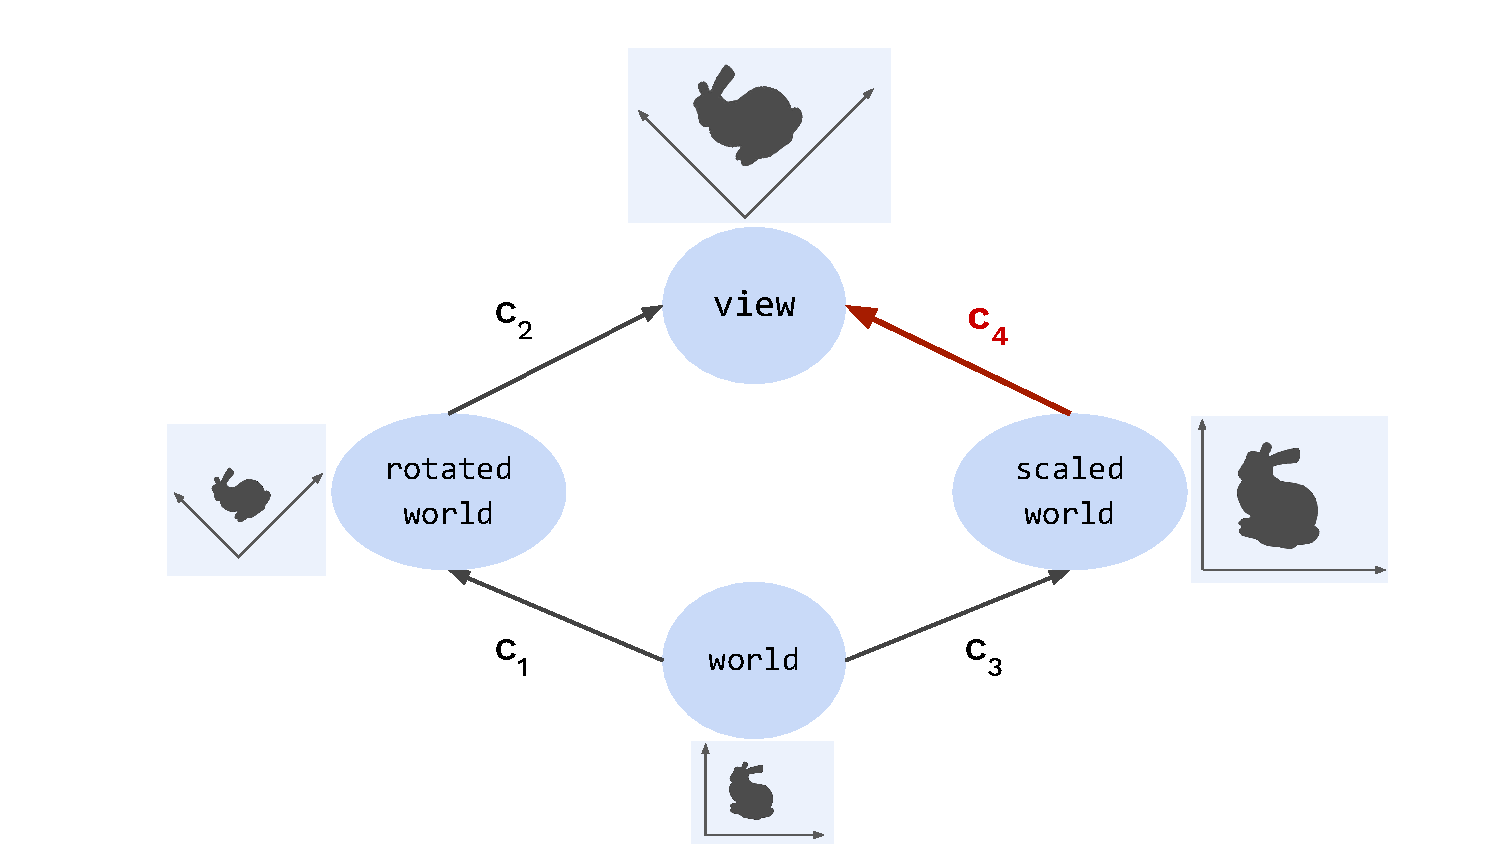
\includegraphics[width=3in]{fig/canonical.pdf}
		\caption{A \emph{transformation graph} with provided transformations. The highlighted edge represents a newly added transformation function, which must be unique and agree with the existing paths on the graph.}
		\label{fig:inpaths}
	\end{minipage}
	\begin{minipage}{.48\linewidth}
		\begin{align*}
			c &\in\text{constants}\\
			x &\in\text{variables}\\
			f &\in \text{function names}\\
			p &\in\text{primitives}\\
			t &\in\text{types} \\
			\tau &\defas \textrm{unit} \,|\, \top_p \,|\, \bot_p \,|\, t \\
			e &\defas v \,|\, c \,|\, f(e_1, e_2) \,|\, x\ \textrm{as!}\ \tau \,|\, x\ \textrm{in}\ \tau\\
			C &\defas \tau \, x = e \,|\, e\\
			P  &=  C;P \,|\, \epsilon\\
		\end{align*}
		\caption{Core Gator syntax.}
		\label{fig:syntax}
	\end{minipage}
\end{figure}
\paragraph{Implementation}
The Gator compiler implements \code{in} expressions by searching for transformations to complete the chain from one type to another.
It uses a \emph{transformation graph} where the vertices are types and the edges are transformation matrices or functions.
Figure~\ref{fig:inpaths} gives a visual representation of a transformation graph.

\subsection{Canonical Functions}
\label{sec:canon}

The transformations that gator reasons about for automatic application are special: they must uniquely define a map from their domain to their range. 
Gator requires these functions to be labeled with the word \code{canon}.
Gator defines three requirements on these transformations:
(1) there can be only one canonical function between each pair of types in a given scope, (2) all canonical functions between reference frames must map between frames of the same dimension, and (3) a canonical function can only have one non-canonical argument.

To expand on condition (3); canonical functions may take in \emph{canonical arguments}, which are variables labelled with the \code{canon} keyword.  The most familiar example of this use is defining matrix---vector multiplication to be canonical; the matrix itself must be included and must be a canonical matrix:
%
\begin{verbatim}
	with frame(3) target:
	canon point *(canon transformation<target> t, point x) {
		...
	}
	...
	// Now declare the matrix as canonical 
	// for use with multiplication
	canon hom<model>.transformation<world> uModel;
	homPos in world; // --> uModel * homPos
\end{verbatim}
%
It is legal to manually fill canonical arguments to functions with non-canonical variables; however, \code{in} expressions will never do so.

The intuition of canonical functions comes from affine transformations between frames and coordinate schemes.
Since each frame has underlying basis vectors, transformations between frames of the same dimension which preserve these frames are necessarily unique; further, applying these bijective transformations does not cause data to ``lose information.''
Similarly, coordinate schemes simply provide different ways to view the same information; there are often unique transformations between schemes that can be applied as needed to unify data representation.

This construction of canonical functions and automatic transformations is similar to constructions provided by C\# and C++'s type coercion.
The slightly different approach needed for \code{in} expressions will be discussed briefly in Section~\ref{sec:rw}.

\subsection{Correctness of Generated Transformations}

With \code{in} expressions, Gator programmers sacrifice control for convenience:
the compiler picks which transformation functions and matrices to use to get from one coordinate system to another.
%
If all the individual transformations marked with \code{canon} are correct, then the composed ``chain'' generated for an \code{in} expression must also be correct.
%
Functional verification of transformations, however, is not feasible in Gator's purely static setting:
it would require not only the value of every transformation matrix, which typically varies dynamically over time,
but also an intrinsic description of each coordinate system, such as the basis vectors for every reference frame, which is never available in real graphics code.
%
We view heavyweight dynamic debugging aids for checking transformation correctness as important future work.

We can, however, state a simple consistency condition that is necessary but not sufficient for a system of canonical transformations to be correct.
%
The transformation system should be \emph{path independent:}
for any two types $\tau_1$ and $\tau_2$, the behavior of any chain of transformations from $\tau_1$ to $\tau_2$ should be equivalent.
%
In other words, every edge in the transformation graph corresponds to a function---so every path corresponds to a function composition,
and every such path between the same two vertices should yield the same composed function.
%
(This definition is equivalent to commutativity for diagrams~\cite{murota}.)
%
Otherwise, the semantics of an expression \code{$e$ in $\tau$} would depend on the graph search algorithm that Gator uses to find routes in the transformation graph, which is clearly undesirable.

Because it is a purely static system, Gator does not enforce path independence.
%
However, path independence motivates Gator's requirement that canonical transformations preserve dimensionality (see Section~\ref{sec:canon}).
%
Without this condition, we have found it is easy to accidentally violate path independence with non-invertible functions and result in an ambiguous transformation graph for \code{in} expressions.
\section{Formal Semantics}
\label{sec:semantics}

% The name of the GLSL-like "target" language.
\newcommand{\targlang}{Hatchling\xspace}

Gator provides a framework for defining geometry types as an ``overlay'' on top of computation-oriented programs in a base language without geometry types.
In this section, we formalize a core of Gator to show that its constructs are sound with respect to such an underlying language.
The goal is a theorem stating that well-typed Gator programs, when translated, result in well-typed programs in the target language.
We focus on the generic, extensible Gator language rather than formalizing the rules for any specific geometric system---affine transformations on Cartesian coordinates, for example.
Proving soundness with respect to a linear algebra domain would be interesting future work but is out of scope for this paper.

We define two languages: a high-level core semantics for Gator that includes its user-defined types, and a low-level abstract target language, \targlang.  \targlang represents a sound imperative language with some set of primitive types and operators on those types.
For example, an instance with fixed-size vector and matrix types can reflect a simple core of GLSL.

\subsection{Syntax}

Figure~\ref{fig:syntax} lists the syntax of the formal core of Gator that we formalize in this section.
The types in this core language consist of \code{unit} and a lattice over each primitive type $p$.
The choice of primitives is kept abstract in this formalism to highlight that the Gator extend over arbitrary underlying datatypes.
For example, in a GLSL core language, we might have a primitive \code{float} or \code{vec3} -- something like \code{vector} would be a custom type $t$ and not a primitive.

A program in Gator is a series of commands; we simplify these to variable declaration, assignment, and expressions.
Gator expressions are constructed around function applications, with \code{as} and \code{in} expressions to help manage types..
We assume functions always take two arguments for simplicity; extending this assumption for other argument counts is straightforward.


\subsection{Typing Rules}
\label{subsec:order}

We define a typing judgment for Gator programs, $\Gamma |- P : \tau$, that, for any program $P$ and typing context $\Gamma$, produces a type $\tau$.  The complete semantics for this judgment can be seen in Figure~\ref{fig:typing}.  
Note that $\Gamma$ is kept constant throughout; declaring a variable requires looking up into the constant $\Gamma$ to determine if the declared type matches the expected type.
Keeping $\Gamma$ constant will later help with translation; the type of any expression can be determined exactly from the constant global contexts $\Gamma,\mathrm{X},\text{and }\Phi$ along with the judgment \textrm{P}.

Gator requires a lattice for each primitive type; custom types on each lattice introduces new subtyping relations.
We define a type ordering among types $\leq$ where $t_1 \leq t_2$ means that $t_1$ is a subtype of $t_2$.
$\leq$ is expected to be reflexive and transitive.
In a well formed program, $\leq$ must contain a rule for every user defined type, every type (except unit) must be a subtype of a primitive top type, and every bottom type $\bot_p$ must be a subtype of each subtype of the associated $\top_p$.
In other words, $\leq$ must conform to a lattice structure for each primitive $p$.
The complete summary of subtyping rules can be found in the attached supplementary materials.

\begin{figure}
	\begin{mathpar}
		\inferrule
		{\tau_1\leq\tau_2\qquad\Gamma\vdash e:\tau_1}
		{\Gamma\vdash e:\tau_2}
		
		\inferrule
		{\textrm{X}(c)=p}
		{\Gamma\vdash c:\bot_p}
		
		\inferrule
		{\Gamma(v)=\tau}
		{\Gamma\vdash x :\tau}
		
		\inferrule
		{\Gamma\vdash e : \tau\qquad\Gamma(v)=\tau}
		{\Gamma\vdash \tau\ x = e:\textrm{unit}}
		
		\inferrule
		{\Gamma\vdash C : \tau_1\qquad\Gamma\vdash P : \tau_2}
		{\Gamma\vdash C;P:\textrm{unit}}
		
		\inferrule
		{ }
		{\Gamma\vdash \epsilon:\textrm{unit}}
		
		\inferrule
		{\Gamma\vdash e: \top_p\qquad\tau\leq\top_p}
		{\Gamma\vdash e\ \textrm{as!}\ \tau:\tau}
		
		\inferrule
		{\Gamma\vdash e : \tau_1\qquad\textrm{P}(\tau_1,\tau_2)=f}
		{\Gamma\vdash e\ \textrm{in}\ \tau_2:\tau_2}
		
		\inferrule
		{\Gamma\vdash e_1:\tau_1\qquad\Gamma,\vdash e_2:\tau_2 \qquad \Phi(f,\tau_1,\tau_2)=\tau_3}
		{\Gamma\vdash f(e_1,e_2):\tau_3}
	\end{mathpar}
	\caption{Typing Judgment}
	\label{fig:typing}
\end{figure}

The typing information for functions is stored in a function typing context, $\Phi$, which maps the tuple of function name and input types to the output type.  The semantics of $\Phi$ are built to support overloaded functions.

Gator, as defined in these semantics, is parameterized over primitive types stored in primitive type context $X$, which maps a literal to its primitive type.

The map from $\mathrm{in}$ expressions to paths is managed by the judgment $\mathrm{P}$.  More precisely, $\mathrm{P}$ maps a given start and end type $\tau_1$ and $\tau_2$ to a function name that, when applied to an expression of type $\tau_1$, produces an expression of type $\tau_2$.  We simplify the judgment of \textrm{P} here to only allow one step for notation clarity; in the real Gator implementation, the transformation may be a chain of functions.  The details of this judgment $\mathrm{P}$ are omitted for simplicity, but amount to a simple lookup through the available functions for a function of the correct type.

\subsection{Translation Soundness}
\begin{figure}
	\begin{align*}
		\source{c}_\Gamma &\triangleq c &
		\source{x}_\Gamma &\triangleq x \\
		\source{\tau\ x := e}_\Gamma &\triangleq \source{\tau}\ x := \source{e}_\Gamma &
		\source{e\ \mathrm{as!}\ \tau}_\Gamma&\triangleq \source{e}_\Gamma \\
		\source{e\ \mathrm{in}\ \tau_2}_\Gamma&\triangleq \source{f(e)}_\Gamma&\text{where }&\Gamma|-e:\tau_1\text{ and }f=\mathrm{P}(e,\tau_1,\tau_2)\\
		\source{f(e_1, e_2)}_\Gamma&\triangleq f'(e_1, e_2)&\text{where }&\Gamma|-e:\tau_1,\Gamma|-e:\tau_2,\text{ and }f'=\Psi(f,e_1,e_2,\tau_1,\tau_2)\\
		\source{\epsilon}_\Gamma&\triangleq \epsilon&
		\source{C;P}_\Gamma&\triangleq\source{C}_\Gamma;\source{P}_\Gamma\\
		\source{t}&\triangleq \top_p&\text{where }t&\leq\top_p\\
		\source{\top_p}&\triangleq \top_p &
		\source{\bot_p}&\triangleq \top_p \\
		\source{\textrm{unit}}&\triangleq \textrm{unit}
	\end{align*}
	\caption{Translational semantics for expressions and types}
	\label{fig:translation}
\end{figure}

To prove the translation soundness of Gator, we need to first define \targlang and our translation from Gator to \targlang.
We will show that a well-typed Gator program must translate to a well-typed \targlang program. 

Primitives in Gator can be translated to a type in the target language. 
For notation convenience we name primitives such that $\top_p$ in Gator translates to $\top_p$ in \targlang.

We define the syntax of \targlang to be identical to Gator syntax except for $\tau$, which is instead written as $\tau::=\mathsf{unit}\,|\,\top_p$, and without $\textrm{as!}$ or $\textrm{in}$ expressions.
In other words, \targlang is simply Gator with custom type labels and associated operations erased.
In the formalism of \targlang, abstraction over operation implementation is done using operation context $\Xi$ that maps an operator name to its output type.

When \targlang is parameterized to be a simple core of GLSL, some top types we might see are the \code{float} and \code{vec3} types.  Translation from Gator would consist of erasing custom geometry types, such as \code{cart3<model>.point}, to their associated top type; in this case \code{vec3}.

To translate Gator's externally-defined functions (which may be overloaded on types not part of \targlang), we invoke the context $\Psi$. 
$\Psi$ maps the tuple of a function name, input expressions, and input types to an expression in the target language. 
For example, we might map Gator's definition of subtraction between points to be a GLSL subtraction between two \code{vec3}s.
The resulting function names must each be unique and preserve the translation of Gator's primitive types.
A well formed function translation context $\Psi$ would necessarily map functions to expressions of the correct return type, as constrained by $\Phi$ under translation.

We reuse the judgment $\mathrm{P}$ as a mechanism to resolve $\mathrm{in}$ expressions, applying the function result of evaluating the judgment to $e$.  This must produce a result of the correct translated type for a well-formed judgment \textrm{P}.

The typing rule for operation expressions is:
%
\begin{mathpar}
	\infer[]
	{\Gamma\vdash o(e_1,e_2):\tau_3}
	{\Gamma\vdash e_1:\tau_1\qquad\Gamma,\vdash e_2:\tau_2 \qquad\Xi(o)=\tau_3}
\end{mathpar}
%
We emphasize this rule as being similar to Gator's rules for operations, but with a ``translated'' context using only \targlang (i.e. primitive) types.  We also note that $\Xi$ does not take in types as arguments, thus \targlang does not support overloaded functions.

We define translational semantics from type-annotated Gator to \targlang in Figure~\ref{fig:translation}. 
The typing contexts $\Gamma$ and $\Phi$ are translated by replacing every $\tau$ in their range with $\llbracket\tau\rrbracket$.

Using structural induction over expressions in Gator, we are now able to show that
\begin{theorem}[translational soundness]
	For all $\Gamma$, $e$, and $\tau$,
	if $\Gamma |- e : \tau$
	then $\source{\Gamma} |- \source{e}_\Gamma : \source{\tau}$.
\end{theorem}
That is to say, if Gator code type checks, then \targlang code type checks.  
Since \targlang is constrained to be sound, Gator must be sound.
A sketch of this proof is included in the provided supplementary materials.
% %
% Appendix~\ref{app:formalism} gives the full translation and proves dimensional safety.

\section{Implementation}
\label{sec:practice}

We implemented Gator in a compiler that statically checks user-defined geometric type systems as described in Section~\ref{sec:langlang} and automatically generates transformation code as described in Section~\ref{sec:in}.
The compiler consists of 2,800 lines of OCaml.
It can emit either GLSL or TypeScript source code, to target either GPU shaders or CPU-side setup code, respectively.

The rest of this section describes how the full Gator language implementation extends the core language features to enable real-world graphics programming.
We demonstrate these features in detail in a series of case studies in Section~\ref{sec:inpractice}.

\subsection{Practical Features}
\label{sec:target}
\paragraph{Types}

While Gator is designed around geometry types, writing realistic code requires a more complete language design.
Aside from the primitive types \code{bool}, \code{int}, \code{float}, and \code{string}, Gator supports fixed-length array types, such as \code{float[3]}, and type aliases.

New types may be declared as a \emph{subtype} of an existing type.
For instance, we can add support for the GLSL-style \code{vec3}:
%
\begin{lstlisting}
type vec3 is float[3];
\end{lstlisting}
%
Through creating a custom type alias, we can, for example, provide support for a subtype of \code{float[3]}, the GLSL \code{vec3}.
While the built-in \code{float[3]} type does not support vector addition, we will be able to write $x+y$ for \code{vec3}s $x,y$ as in GLSL.

To allow literal values to interact intuitively with custom types, literals in Gator have special types.
For example, the number $42$ is of type \code{%int}.
Gator introduces a typing rule where each literal type $\%p$ is a subtype of every subtype of $p$.  In other words, the literal type $\%p$ is the bottom type for the type hierarchy with top type $p$.
We summarize these ideas in this example:
%
\begin{lstlisting}
type vec3 is float[3];
vec3 s1 = [4.2, 4.2, 4.2];  // Legal 
float[3] x = s1;            // Legal
vec3 s2 = x;                // ERROR: float[3] is not a vec3
\end{lstlisting}
%
This behavior of literal values allows us to capture the Gator-style intuition that a given vector can either be a geometric point or just a raw GLSL \code{vec3}, but this information is not known until the data is assigned to a variable.
\paragraph{Type Inference}
Gator supports local type inference using the \code{auto} keyword:
%
\begin{lstlisting}
cart3<model>.point fragPos = ...;
// worldPos will have type cart3<world>.point
auto worldPos = fragPos in world;
\end{lstlisting}
%
\paragraph{External Functions}
Functions and variables defined externally in the Gator target can be written using the \code{declare} keyword.
%
\begin{lstlisting}
declare vec3 normalize(vec3 v);
\end{lstlisting}
%
All arithmetic operations in Gator are functions which can be declared and overloaded.
Gator has no built-in functions.
Requiring this declaration allows us to include GLSL-style infix addition of vectors without violating coordinate systems restrictions:
%
\begin{lstlisting}
	declare vec3 +(vec3 v1, vec3 v2);
\end{lstlisting}
%
Addition is then valid for values of type \code{vec3}:
%
\begin{lstlisting}
vec3 x = [0., 1., 2.];
vec3 result = x + x; // Legal
\end{lstlisting}
%
But emits an error when applied to two points, as desired, since they are not subtypes of vec3 and so there is no valid function overload:
%
\begin{lstlisting}
cartesian<model>.point fragPos = [0., 1., 2.];
// ERROR: No addition defined for points
auto result = fragPos + fragPos; 
\end{lstlisting}
%
\paragraph{Import System}
To support using custom Gator libraries in a readable way, we built a simple import system in Gator.  Files can be imported with the keyword \code{using} followed by the name of the file:
%
\begin{lstlisting}
using "../glsl_defs.lgl";
\end{lstlisting}
%
\paragraph{Unsafe Casting}
As an escape hatch from strict vector typing, Gator provides an unsound cast expression written with \code{as!}:
%
\begin{lstlisting}
vec3 position = fragPos as! vec3;
\end{lstlisting}
%
Casts must preserve the primitive representation; we could not, for instance, cast a variable with type \code{float[2]} to \code{float[3]}.
Unsafe casts syntactically resemble \code{in} expressions but are unsound and carry no run-time cost.
These casts both allow for unsafe transformations for defining a function that is externally ``known'' to be safe, and for allowing the user to forgo Gator's type system and work directly with GLSL-like semantics, as seen in the example above.

\subsection{Standard Library}
Per Section \ref{sec:semantics}, Gator does not include any built-in functions or operations.  Our implementation does provide array indexing as a built-in function to help simplify definitions, but otherwise matches requires that operations such as \code{+} be explicitly declared.

We implement a standard library provides access to common GLSL operations.  This library consists of GLSL function declarations, scheme declarations for Cartesian and Homogeneous coordinates, and basic transformation functions such as \code{homify} and \code{reduce}.  Relevant GLSL functions are declared to work on GLSL types, such as the addition operation operation in section~\ref{sec:practice}:
%
\begin{lstlisting}
declare vec3 +(vec3 x, vec3 y);
\end{lstlisting}
%
We build schemes in much the same way as introduced in Section~\ref{subsec:schemes}, as with the sketch of the \code{cart3} scheme:
%
\begin{lstlisting}
with frame(3) r:
coordinate cart3 : geometry {
  object vector is float[3];
  vector +(vector v1, vector v2) {
	return [
	  v1[0] + v2[0], 
	  v1[1] + v2[1], 
	  v1[2] + v2[2]];
  }
}
\end{lstlisting}
%
Finally, we include \code{homify} and \code{reduce} transform between homogeneous and cartesian coordinates as discussed in Section~\ref{subsec:objects}:
%
\begin{lstlisting}
hom<model>.point homify(cart3<model>.point p) {
  return [p[0], p[1], p[2], 1.]; 
}
cart3<model>.point reduce(hom<model>.point p) {
  return [p[0], p[1], p[2]]; 
}
\end{lstlisting}
%
We use this same library when implementing each shader for the case study.
\section{Gator in Practice}
\label{sec:inpractice}

This section explores how Gator can help programmers avoid geometry bugs using a series of case studies.
We use the Gator compiler to implement OpenGL-based renderers that demonstrate a variety of common visual effects,
and we compare against implementations in plain GLSL.
We report qualitatively on how Gator's type system influences the expression of the rendering code (Section~\ref{sec:casestudies} and quantitatively on the performance impact of Gator's \code{in} expressions (Section~\ref{sec:performance}).

\subsection{Case Studies}
\label{sec:casestudies}

\begin{figure}
\centering
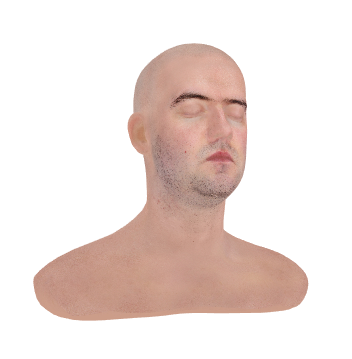
\includegraphics[width=\linewidth]{fig/texture.png}
\caption{Texture.}
\label{fig:texture}
\end{figure}
\begin{figure}
		\centering
		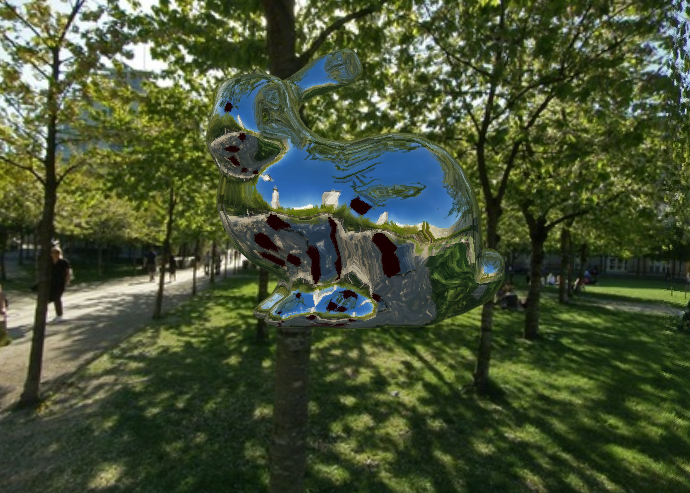
\includegraphics[width=\linewidth]{fig/reflection.png}
		\caption{Reflection.}
		\label{fig:reflection}
\end{figure}
	
\begin{figure}
		\centering
		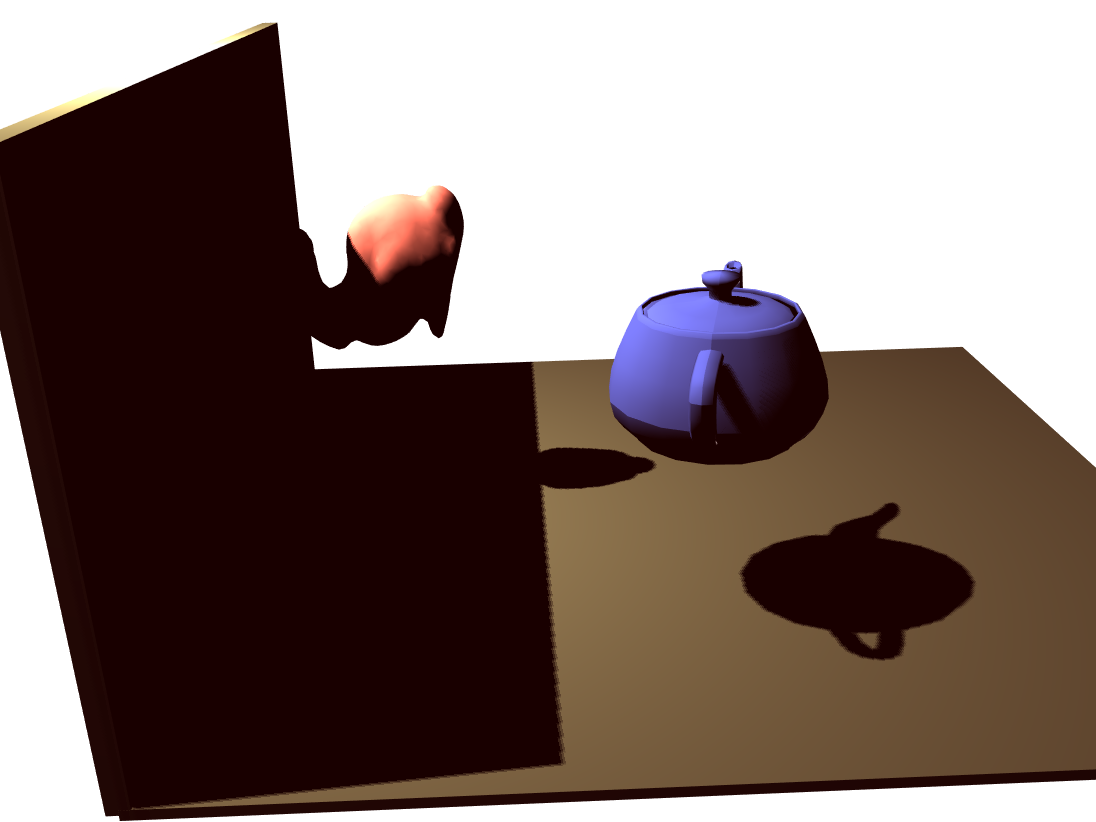
\includegraphics[width=\linewidth]{fig/shadowmap.png}
		\caption{Shadow map.}
		\label{fig:shadowmap}
\end{figure}
\begin{figure}
		\centering
		
\includegraphics[width=\linewidth]{fig/microfacet.png}
		\caption{Microfacet.}
		\label{fig:microfacet}
\end{figure}

% This stuff seems like a rehash of things we've already said above---no need
% to repeat. --A
% To evaluate Gator's expressiveness and effectiveness at ruling out geometry bugs, we implemented a compiler from Gator to GLSL and used it to create a series of standard shader implementations.
% To help normalize the differences between Gator and GLSL, we include a GLSL-specialized standard library and basic import system as described above in section~\ref{sec:target}.

To qualitatively study Gator's safety and expressiveness, we used it to implement 8 renderers based on the OpenGL API in its browser-based incarnation, WebGL~\cite{webgl}.
To the best of our knowledge, there is no standard benchmark suite for evaluating the expressiveness and performance of graphics shader programs.
Instead, we assemble implementations of a range of common rendering effects:
%
\begin{itemize}
	\item \emph{Phong:} The lighting model introduced in Section~\ref{sec:example}.
	\item \emph{Reflection:} Use two-pass rendering to render an object that reflects its surroundings.
	\item \emph{Shadow map:} Simulate shadows for moving objects by computing a projection.
	\item \emph{Microfacet:} Texture model for simulating roughness on a surface.
	\item \emph{Texture:} Use OpenGL's texture mapping facility to draw an image on the surface of an object.
	\item \emph{Spotlight:} Phong lighting restricted to a spotlight circle.
	\item \emph{Fog:} Lighting model with integration to simulate distortion from fog.
	\item \emph{Bump map:} Texture model for simulating bumps on surfaces.
	%\item \emph{Multiple lights:} Multiple lights with shadows to stress geometry transformations.
\end{itemize}
%
Each renderer consists of both CPU-side ``host'' code and several GPU-side shader programs.
Figure~\ref{fig:examples} depicts the output of a selection of these renderers.
% I wrote this sentence but I think it's superfluous. --A
% We compare against baseline implementations using TypeScript and GLSL to show how Gator's type system can eliminate potential pitfalls in those standard languages.

The rest of this section reports on salient findings from the case studies and compares them to standard implementations in GLSL and TypeScript.
For the sake of space, we highlight the most distinct cases where Gator helped clarify geometric properties and prevent geometry bugs that would not be caught by plain GLSL.  The complete code of both the Gator and reference GLSL implementations can be found online.\footnote{URL omitted for anonymous review}

\paragraph{Reflection}

Our reflection case study, shown in Figure~\ref{fig:reflection}, renders an object that reflects the dynamic scene around it, creating a ``mirrored'' appearance.
The surrounding scene includes a static background texture, known as a \emph{skybox}, and several non-reflective floating objects to demonstrate how the reflected scene changes dynamically.

Rendering a reflection effect requires several passes through the graphics pipeline.
The idea is to first render the scene that the mirror-like object will reflect, and then render the scene again with that resulting image ``painted'' onto the surface of the object.
There are three main phases:
(1) Render the non-reflective objects from the perspective of the reflective object.
This requires six passes, one for each direction in 3-space.
(2) Render the reflection using the generated cube as a texture reference.
(3) Finally, render all other objects from the perspective of the camera.

\paragraph{Reflection: Inverse Transformation}
For the second step, we refer to a cubemap---a special GLSL texture with six sides---to refer to the six directions of the scene.  
To calculate the angle of reflection, we need to reason about the interactions of the light rays in view space \emph{as they map onto our model space}.  
Specifically, calculating the reflection amounts to the following operations, where \code{V} is the current vertex's position and \code{N} is the current normal vector, which must both be in the view frame:
%
\begin{lstlisting}
uniform samplerCube<alphaColor> uSkybox;
...
void main() {
  ...
  cart3<view>.vector R = -reflect(V, N);
  auto gl_FragColor = textureCube(uSkybox, R in model);
}
\end{lstlisting}
%
The key feature to note here is the transformation \code{R in model}, which accomplishes our goal of returning the light calculation to the object's perspective (the model frame).
This transformation requires that we map backwards through the world frame, a transformation which requires the inverse of the \code{model}$\rightarrow$\code{world} matrix and the \code{world}$\rightarrow$\code{view} matrix multiplied together.
This interaction produces a unique feature in Gator's type system, where we need to both have a forward transformation and its inverse.
The shader declares the matrices as follows, with the inversion being done preemptively on the CPU:
%
\begin{lstlisting}
canon uniform hom<world>.
  transformation<view> uView;
canon uniform hom<model>.
  transformation<world> uModel;
canon uniform cart3<view>.
  transformation<model> uInverseViewTransform;
\end{lstlisting}
%
The inverse view transform uses a Cartesian (\code{cart3}) matrix because
we intend only to use it for the vector \code{R}, which ignores the translation component of the affine transformation.  The inverse transformation is what permits us to write \code{R in model}, while the forward transformations must be uniquely given to actually send our position and normal to the view frame (as noted before):
%
\begin{lstlisting}
varying cart3<model>.point vPosition;
varying cart3<model>.normal vNormal;
void main()
auto N = normalize(vNormal in view);
auto V = -(vPosition in view);
...
}
\end{lstlisting}
%
\paragraph{Reflection: Normal Transformation}
Additionally, we need to reason about the correct transformation of the normal \emph{with translation} (that is, when moving the object in space), which means that we need the inverse transpose matrix, which provides a distinct path between the model and view frames.  The use of the inverse transpose of the model-view matrix is perhaps unexpected; it arises specifically for a geometry normal from a convenient algebraic result.

In GLSL, it is easy to mistakenly transform the normal as if it were an ordinary direction:
%
\begin{lstlisting}
varying vec3 vNormal;
void main() {
  auto N = normalize(vec3(
    uView * uModel * vec4(vNormal, 0.)));
}
\end{lstlisting}
%
This code is wrong because \code{uModel * vec4(vNormal, 0.)} does not apply the translation component of the \code{uModel} transformation.
To prevent this kind of bug, the Gator standard library defines the \code{normal} type, which is a subtype of \code{vector}.
A new \code{normalTransformation} type can only operate on normals.
Using these types, a simple \code{in} transformation suffices:
%
\begin{lstlisting}
canon uniform cart3<model>.
  normalTransformation<view> uNormalMatrix;
varying cart3<model>.normal vNormal;
void main() {
  // uNormalMatrix * vNormal
  auto N = normalize(vNormal in view);  
}
\end{lstlisting}
%
The compiler uses the normal version of the transformation, correctly applying the translation component.

\paragraph{Shadow Map: Light Space}
Shadow mapping is a technique to simulate the shadows cast by 3D objects when illuminated by a point light source.  Our case study, shown in Figure~\ref{fig:shadowmap}, renders several objects that cast shadows on each other and a single ``floor'' surface.  The non-shadow coloring is simulated through Phong lighting as previously discussed.

As with the reflection renderer, to calculate shadows in a scene, we require several passes through the graphics pipeline.  The first pass renders the scene from the perspective of the \emph{light} and calculates the whether a given pixel is obscured by another.  The second pass uses this information to draw shadows; a given pixel is lit only if it is not obscured from the light.

The first pass does all geometric operations in the vertex shader to render the scene from the light's perspective.  This is easy to get wrong in GLSL by defaulting to the usual transformation chain:
%
\begin{lstlisting}
void main() {
  // The usual transformation chain here is wrong!
  // We should instead be using 
  //    uLightProjective and uLightView
  vec4 gl_Position = uProjective * 
    uView * uModel * vec4(aPosition, 1.);
}
\end{lstlisting}
%
This incorrect transformation chain will lead to shadows in strange places and hard-to-debug effects.

In Gator, on the other hand, the work is done when typing the matrices themselves.  From there, the transformation to light space is both documented and correct by construction:
%
\begin{lstlisting}
attribute cart3<model>.point aPosition;
canon uniform hom<model>.
  transformation<world> uModel;
canon uniform hom<world>.
  transformation<light> uLightView;
canon uniform hom<light>.
  transformation<lightProjective> uLightProjection;

void main() {
auto gl_Position = aPosition in hom<lightProjective>;
// ...
}
\end{lstlisting}
We use the depth information in the final pass in the form of \code{uTexture}.  To look up where the shadow should be placed, we must lookup the position of the current pixel in the light's projective space (which is where the position was represented in the previous rendering).
In GLSL, we require the following hard-to-read code:
\begin{lstlisting}
float texelSize = 1. / 1024.;
float texelDepth = texture2D(uTexture, 
vec2(uLightProjective * uLightView * 
  uModel * vec4(vPosition, 1.))) + texelSize));
\end{lstlisting}
Using the correct transformations is difficult and hard to be sure if the correct transformation chain was used once again.  In Gator, on the other hand, this is straightforward:
\begin{lstlisting}
float texelSize = 1. / 1024.;
float texelDepth = texture2D(uTexture, 
  vec2(vPosition in lightProjective) + texelSize));
\end{lstlisting}

\paragraph{Microfacet: Custom Canonical Functions}

Anisotropic microfacet shading creates an illusion of roughness and bumpiness on a 3D modeled surface using information from the normal map of that surface.  Modeling this correctly, however, requires an unusual technique: building a local reference frame from the perspective of the normal vector called the local normal frame.

Converting to the local normal frame of a given normal consists of a function call with the appropriate normal vector.
%
\begin{lstlisting}
vec3 proj_normalframe(vec3 m, vec3 n) { ... }
vec3 geom_normal;
vec3 result = proj_normalframe(viewDir, geom_normal);
\end{lstlisting}
%
However, as with other conversions between spaces,
writing this kind of code in GLSL can
involve multiple nonobvious steps.
If the normal and target direction are in different spaces, the GLSL code must look like this:
%
\begin{lstlisting}
vec3 result = proj_normalframe(vec3(uView * 
  uModel * vec4(modelDir, 1.)), geom_normal);
\end{lstlisting}
%
In Gator, we instead declare \code{proj_normalframe} with the appropriate types and a canonical tag, noting that the normal itself is a canonical part of the transformation:
%
\begin{lstlisting}
frame normalframe has dimension 3;
canon cart3<normalframe>.direction proj_normalframe(
cart3<view>.direction m, canon cart3<view>.normal n) { ... }
\end{lstlisting}
%
We then declare the normal \code{geom_normal} with the appropriate type, and the transformation type becomes straightforward:
%
\begin{lstlisting}
canon cart3<view>.normal geom_normal;
auto result = modelDir in normalframe;
\end{lstlisting}
%
\paragraph{Textures: Parameterized Types}
A \emph{texture} is an image that a renderer maps onto the surface of a 3D object, creating the illusion that the object has a ``textured'' surface.
Our texture case study renders a face mesh with a single texture (shown in Figure~\ref{fig:texture}).
While this example does not provide any geometry insight, we highlight the study to show the broad utility of the types introduced by Gator for a graphics context.
GLSL represents a texture using a \code{sampler2D} value, which acts as a pointer to the requested image, which is typically an input to a shader:
%
\begin{lstlisting}
uniform sampler2D uTexture;
\end{lstlisting}
%
Textures are mapped to the image using the object's current texture coordinate:
%
\begin{lstlisting}
varying vec2 vTexCoord;
\end{lstlisting}
%
Whereas textures themselves are typically constant (using the \code{uniform} keyword), a texture coordinate like \code{vTexCoord} differs for each vertex in a mesh (as the \code{varying} keyword indicates).
To sample a color from a texture at a specific location, a fragment shader must use the GLSL \code{texture2D} function:
%
\begin{lstlisting}
vec4 gl_FragColor = texture2D(uTexture, vTexCoord);
\end{lstlisting}
%
The result type of \code{texture2D} in GLSL is \code{vec4}: while textures typically contain colors (consisting of red, green, blue, and alpha channels), renderers can also use them to store other data such as shadow maps or even points in a coordinate system.

In Gator and its GLSL standard library, \code{sampler2D} is a polymorphic type that indicates the values it contains:
\begin{lstlisting}
with float[4] T:
declare type sampler2D;
with float[4] T:
declare T texture(sampler2D<T> tex, vec2 uv);
\end{lstlisting}
For this renderer, the texture contains \code{alphaColor} values, which represent color values that can be used as \code{gl_FragColor}.
The fragment shader is nearly identical to GLSL but with more specific types:
%
\begin{lstlisting}
uniform sampler2D<alphaColor> uTexture;
varying vec2 vTexCoord;
void main() {
  alphaColor gl_FragColor = texture2D(uTexture, vTexCoord);
}
\end{lstlisting}
%
With this code, we guarantee that the texture represented by \code{uTexture} will produce a color which can be directly used by \code{gl_FragColor}.  We therefore both provide documentation and prevent errors with trying to use the resulting vector as, say, a point for later calculations.

\subsection{Performance}
\label{sec:performance}

While Gator is chiefly an ``overhead-free'' wrapper that expresses the same semantics as an underlying language,
there is one exception where Gator code can differ from plain GLSL:
its automatic transformation insertion using \code{in} expressions (Section~\ref{sec:in}).

The Gator implementation compiles \code{in} expressions to a chain of transformation operations that may be slower than the equivalent in a hand-written GLSL shader.
In particular, hand-written GLSL code can store and reuse transformation results or composed matrices, while the Gator compiler does not currently attempt to do so.
The Gator compiler also generates function wrappers to enable its overloading.
While both patterns should be amenable to cleanup by standard compiler optimizations,
this section measures the performance impact by comparing Gator implementations of renderers from our case study to hand-optimized GLSL implementations.

\subsubsection{Experimental Setup}

We perform experiments on Windows 10 version 1903 with an Intel i7-8700K CPU, NVIDIA GeForce GTX 1070, 16 GB RAM, and Chrome 81.0.4044.138.
We run 60 testing rounds, each of which executes the benchmarks in a randomly shuffled order.
In each round of testing, we execute each program for 20 seconds while recording the time to render each frame.
We report the mean and standard deviation of the frame rate across all rounds.

\subsubsection{Performance Results}

\begin{figure}
\centering
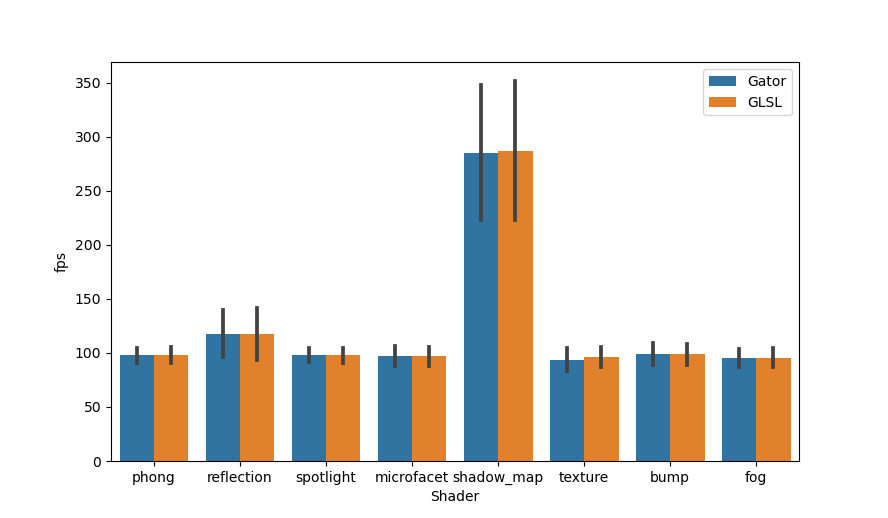
\includegraphics[width=\linewidth]{fig/evalresultsgator.png}
\caption{The mean frames per second (fps) for each shader for both the baseline (GLSL) and Gator code. Error bars show the standard deviation.}
\label{fig:runtime-results}
\end{figure}
\begin{figure}
\centering
\begin{tabular}{ccccccc}
& \multicolumn{2}{c}{Gator} & \multicolumn{2}{c}{GLSL} & \multicolumn{2}{c}{$p$-value} \\
\cmidrule(r){2-3} \cmidrule(r){4-5} \cmidrule(r){6-7}
Shader & Mean & S.E. & Mean & S.E. & Wilcoxon & TOST \\
\midrule
\bmark{phong}      & 97.84 & 0.22 & 97.67 & 0.21 & 0.187    & 0.003*\\
\bmark{texture}    & 95.82 & 0.27 & 93.75 & 0.31 & $<$0.001*& 0.996\\
\bmark{reflect}    & 117.8 & 0.72 & 117.7 & 0.65 & 0.638    & 0.188\\
\bmark{shadow}     & 287.0 & 1.91 & 285.1 & 1.85 & 0.365    & 0.636\\
\bmark{bump}       & 98.60 & 0.29 & 99.07 & 0.29 & 0.063    & 0.098\\
\bmark{microfacet} & 96.71 & 0.27 & 96.91 & 0.28 & 0.640    & 0.020*\\
\bmark{fog}        & 95.74 & 0.26 & 95.41 & 0.25 & 0.119    & 0.033*\\
\bmark{spotlight}  & 97.83 & 0.21 & 98.07 & 0.20 & 0.299    & 0.005*\\
\bottomrule
\end{tabular}
\captionof{table}{Mean and standard error of the frame rate for the Gator and GLSL (baseline) implementation of each benchmark. We also give the $p$-value for a Wilcoxon sign rank test and two one-sided $t$-test (TOST) equivalence test that checks whether the means are within 1~fps, where * denotes statistical significance ($p < 0.05$).}
\label{tab:perf-results}
\end{figure}

Figure~\ref{fig:runtime-results} shows the average frames per second (fps) for the GLSL and Gator versions of each renderer, and Table~\ref{tab:perf-results} shows mean and standard deviation of each frame rate.
The frame rates for the two versions are generally very similar---the means are all within one standard deviation.
% within 1~fps, except for \bmark{shadow}, which has a particularly high variance, and \bmark{texture}, which we discuss in more detail below.
Several benchmarks have frame rates around 100~fps because they render the same number of objects and the bulk of the cost comes from scene setup.
% Many of the results appear clustered around 100~FPS; this is due to testing taking place with similar number of objects for each.
% While the shaders provide variation in frame rate, the bulk of the frame cost is the size of the scene being setup.
We used around 100 objects for all scenes except \bmark{reflection} and \bmark{shadow} to reduce natural variation and focus on measuring the cost of the shaders.

Table~\ref{tab:perf-results} shows the results of Wilcoxon signed-rank statistical tests that detect differences in the mean frame rates.
At an $\alpha = 0.05$ significance level, we find a statistically significant difference only for \bmark{texture}.
However, a difference of means test cannot \emph{confirm} that a difference does \emph{not} exist.
For that, we also use we use the two one-sided $t$-test (TOST) procedure~\cite{tost}, which yields statistical significance ($p < \alpha$) when the difference in means is within a threshold.
We use a threshold of 1~fps.
The test rejects the null hypothesis---concluding, with high confidence, that the means are similar---for the \bmark{phong}, \bmark{microfacet}, \bmark{fog}, and \bmark{spotlight} shaders.

The anomaly is \code{texture}, where our test concludes that a small (2~fps) performance difference does exist, although the differences are still within one standard deviation.
Our best guess as to the reason is due to a result of the boilerplate functions inserted by Gator, some of which be optimized away with more work.

\section{Related Work}
\label{sec:rw}

SafeGI~\cite{safegi} introduces a type system as a C/C++ library for geometric objects parameterized on reference frame labels not unlike Gator's geometry types.  The types introduced by SafeGI do not include information about the coordinate scheme, and so also requrie abstracting the notion of transformations to a map type which must be applied through a layer of abstraction.  
Additionally, SafeGI does not attempt to introduce automatic transformations like Gator's \code{in} expressions nor attempt to study the result of applying these types to real code.

The dominant mainstream graphics shader languages are OpenGL's GLSL~\cite{glsl} and Direct3D's HLSL~\cite{direct3d}.
Research on graphics-oriented languages for manipulating vectors dates at least to Hanrahan and Lawson's original \emph{shading language}~\cite{hanrahan90}.
Recent research on improving these shading languages has focused on modularity and interactions between pipeline stages:
Spark~\cite{spark} encourages modular composition of shaders;
Spire~\cite{spire} facilitates rapid experimentation with implementation choices;
and Braid~\cite{braid} uses multi-stage programming to manage interactions between shaders.
These languages do not address vector-space bugs.
Gator's type system and transformation expressions are orthogonal and could apply to any of these underlying languages.

Scenic~\cite{spatial} introduces semantics to reason about relative object positions and $\lambda$CAD~\cite{acad} introduces a small functional language for writing affine transformations, although neither seem to have a type system for checking the coordinate systems they've defined.
Practitioners have noticed that vector-space bugs are tricky to solve and have proposed using a naming convention to rule them out~\cite{naming}.
A 2017 enumeration of programming problems in graphics~\cite{lfogl} identifies the problem with latent vector spaces and suggests that a novel type system may be a solution.
Gator can be seen as a realization of this proposal.

Gator's type system works as an overlay for a simpler, underlying type system that only enforces dimensional restrictions.
This pattern resembles prior work on type qualifiers~\cite{cqual}, dimension types~\cite{dimension}, and type systems for tracking physical units~\cite{unit}.
Canonical transformations in Gator are similar in feel to Haskell's type class polymorphic functions, where Gator's \code{space} type can be defined as a type class and the \code{in} keyword behave similarly to Haskell lookup calls.
Additionally, Gator's notion of automatic transformations is a specialized use type coercion, similar to structures introduces in the C\# and C++ languages.
What is particular about Gator's automatic type coercion is the notion of path independence discussed in Section~\ref{sec:in}, along with a definition of uniqueness and bijectivity of canonical transformations. Together, these requirements allow automation of coordinate system transformations that would not be allowed in other, similar systems.

\section{Conclusion}

Gator attacks a main impediment to graphics programming that makes it hard to learn and makes rendering software hard to maintain.
Geometry bugs are extremely hard to catch dynamically, so Gator shows how to bake them into a type system and how a compiler can declaratively generate ``correct by construction'' geometric code.
We see Gator as a foundation for future work that brings programming languages insights to graphics software,
such as formalizing the semantics of geometric systems
and providing abstractions over multi-stage GPU pipelines.

Geometry bugs are not just about graphics, however.
Similar bugs arise in fields fields ranging from robotics to scientific computing.
In Gator, users can write libraries to encode domain-specific forms of geometry: affine, hyperbolic, or elliptic geometry, for example.
We hope to expand Gator's standard library as we apply it to an expanding set of domains.

\bibliography{venues,refs}


\chapter{Online Verification of Commutativity}

%\documentclass[../main.tex]{subfiles}
%

\section{Introduction}
\label{introduction}
Many systems use diagrams: graphs where nodes are domains and edges are transformation functions.
A type system with coercions, for example, corresponds to a graph whose nodes are types and whose edges are coercions.
Figure~\ref{fig:typeExample} illustrates an example in a simple language with units-of-measure types~\cite{unitsOfMeasure}.
In such a system, an important correctness criterion is that the diagram \emph{commutes}: when traversing the graph from any start node to any end node, applying every transformation along the path to any input value, the result is the same output value \emph{independent of the path chosen between the two nodes}.
With our coercion example, it is a problem if casting to a supposedly equivalent type as an intermediate step resulted in a different answer than a direct cast.
Specifically, given a variable \code{x} of type \code{meters}, applying the cast \code{(wugs) x} can be done in two ways: either \code{(wugs)(feet) x} or \code{(wugs)(miles) x}.
Which path is taken depends on the compiler; we would like the choice of paths to be semantically equivalent so the compiler is free to make a choice.

\begin{figure}[]
    \begin{verbatim}
var x : meters = 1;
define foot:
    1 meter = 3.28 feet;
define miles:
    1 meter = 0.000621 miles;
define wugs:
    1 mile = 10000 wugs;
    1 foot = 10 wugs;
var y : wugs = (wugs) x;
    \end{verbatim}
\caption{A sample program with user defined type conversion.}
\end{figure}
%
\begin{figure}
    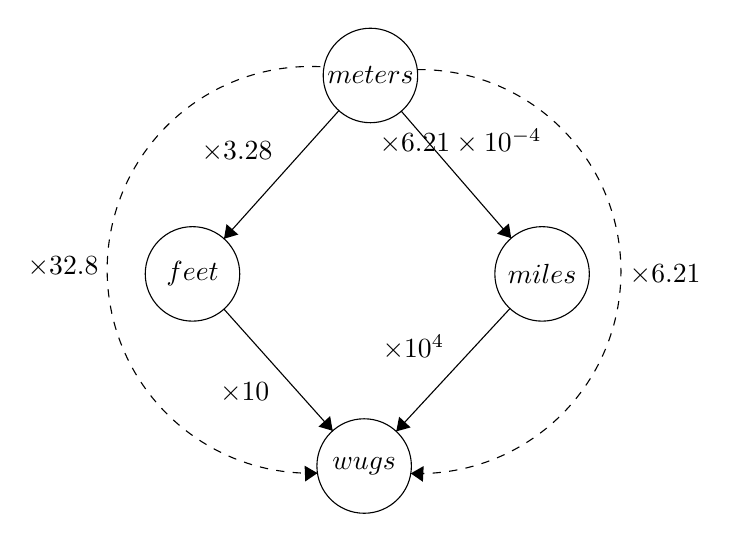
\begin{tikzpicture}[scale=0.2]
        \tikzstyle{every node}+=[inner sep=0pt]
        \draw [black] (32.8,-8.8) circle (3);
        \draw (32.8,-8.8) node {$meters$};
        \draw [black] (21.5,-21.4) circle (3);
        \draw (21.5,-21.4) node {$feet$};
        \draw [black] (43.7,-21.4) circle (3);
        \draw (43.7,-21.4) node {$miles$};
        \draw [black] (32.4,-33.6) circle (3);
        \draw (32.4,-33.6) node {$wugs$};
        \draw [black] (30.8,-11.03) -- (23.5,-19.17);
        \fill [black] (23.5,-19.17) -- (24.41,-18.9) -- (23.66,-18.24);
        \draw (26.61,-13.64) node [left] {$\times 3.28$};
        \draw [black] (34.76,-11.07) -- (41.74,-19.13);
        \fill [black] (41.74,-19.13) -- (41.59,-18.2) -- (40.84,-18.85);
        \draw (43.7,-13) node [left] {$\times 6.21 \times 10^{-4}$};
        \draw [black] (23.5,-23.64) -- (30.4,-31.36);
        \fill [black] (30.4,-31.36) -- (30.24,-30.43) -- (29.5,-31.1);
        \draw (26.41,-28.96) node [left] {$\times 10$};
        \draw [black] (41.66,-23.6) -- (34.44,-31.4);
        \fill [black] (34.44,-31.4) -- (35.35,-31.15) -- (34.62,-30.47);
        \draw (37.52,-26.04) node [left] {$\times 10^4$};
        \draw [dashed] (29.441,-34.049) arc (-88.02206:-273.82603:12.915);
        \fill [black] (29.44,-34.05) -- (28.62,-33.58) -- (28.66,-34.58);
        \draw (15.56,-20.93) node [left] {$\times 32.8$};
        \draw [dashed] (35.77,-8.425) arc (90.49177:-92.33986:12.828);
        \fill [black] (35.36,-34.07) -- (36.13,-34.6) -- (36.18,-33.6);
        \draw (49.23,-21.46) node [right] {$\times 6.21$};
    \end{tikzpicture}
    \caption{In this sample program, the user implicitly defines two ways to cast variable a from meters to the new unit wugs.
    The definitions are different, and a compiler performing implicit conversion would not know which to choose.}
    \label{fig:typeExample}
\end{figure}
%
This paper is about efficiently checking commutativity in diagrams that arise in real systems.
We assume a simple equivalence checker for individual transformation functions: in our type system example, for instance, it is possible to check transformation equivalence by comparing the conversion factors.
Our aim is to analyze the graph of transformations and minimize the number of times we need to perform an equivalence check.
Since diagrams may change over time in real systems, as new conversions are added, and verifying the entire system from scratch may be computationally expensive, we want an online method that only checks the impact of new edges.
In Figure~\ref{fig:typeExample}, for example, a run-time system can catch the point where the programmer adds a bad conversion definition by verifying each new conversion edge as it is created.

Efficient commutativity checking is not trivial.
The presence of cycles implies a potentially infinite number of paths..
Further, na\"{i}vely checking if all path pairs that begin and end at the same node in a given diagram commute could require a number of function equality checks that grow as factorial in the number of nodes, because a path consists of an ordering of nodes.
Previous work ~\cite{commutative} has identified an $O(|E|^2|V|^4)$ algorithm to verify that a complete acyclic diagram commutes; however, it addresses neither online addition nor cyclic diagrams.

For verifying commutativity over online addition, we identify two key insights.
First, when a new edge is added, only one path per source and sink pair needs to be checked against the existing commutative diagram.
Because the diagram commutes, all the paths between a given source and sink are equal and a representative to check against can arbitrarily be chosen.
This leads to an $O(|V|^2(|E|+|V|))$ algorithm to verify a diagram remains commutative over the course of online addition, assuming an oracle to check the equality of functions.
The algorithm makes an \emph{asymptotically} optimal number of calls to the oracle.

Second, there is a single rule that places a partial, transitive ordering on paths indicating the amount of information they contain about other paths.
This insight yields a greedy $O(|V|^4)$ optimization step that results in the number of oracle calls being exactly minimal.
The optimization is critical when equality checking is expensive.

We evaluate our algorithms against random graphs and use them in two case studies.
First, we use our algorithm in the domain specific geometry type language \textit{Gator} ~\cite{gator} to ensure that user defined transformations between spaces stay consistent.
Second, we use our algorithm to identify inefficiencies in a currency conversion graph.
%
We empirically compare our solution to three baseline implementations: a na\"{i}ve cycle-sensitive all-pairs check, a check for all path pairs that involve the new edge, and an algorithm suggested by previous work to solve the batch version of the problem for acyclic diagrams.
Our proposed algorithms run orders of magnitude faster than the baseline implementations.

\section{Formal Problem Setup and Terminology}

We start by formalizing the notion of a diagram, drawing terminology from the previous acyclic work by Murota~\cite{commutative}.

\paragraph{Notation.}

We start with a directed graph $G=(V,E)$, where $V$ corresponds to sets of elements and edges $(u, v)$ in $E$ correspond to functions that maps elements of $u$ to elements in $v$.
These functions form a semigroup $\mathcal{F}$, where multiplication is function composition.
A semigroup consists of a set and an associative binary operation, which we use to capture function composition.
%
The correspondence between edges and functions is stored as a mapping $f:E\rightarrow F$, where $f$ maps each edge to the function it represents.

A path is a sequence of edges. The edge-to-function mapping $f$ can be naturally extended to paths: if path $p$=$e_1 ; \cdots ; e_n$ then $f(p)=f(e_1) ; f(e_2) ; \cdots ; f(e_n)$.
%
We write $\partial(p)^{+}$ for $p$'s start node, $\partial(p)^{-}$ for its end node, and $\partial(p)$ to denote the pair
$(\partial(p)^{+}, \partial(p)^{-})$.

A pair of paths $p_1$ and $p_2$ is said to \textit{parallel} iff their terminal nodes are the same, i.e., $\partial(p_1)=\partial(p_2)$.
$\partial$, $\partial^{+}$ and $\partial^{-}$ are extended to apply to parallel pairs.
For parallel pair $\phi$ = ($p_1$, $p_2$), $\partial(\phi)=\partial(p_1)=\partial(p_2)=(\partial(\phi)^{+}, \partial(\phi)^{-})$.

Let $\mathcal{R}_{all}$ be the set of all parallel pairs of paths in a given diagram.
The diagram commutes iff
$\forall (p_1,p_2)\in \mathcal{R}_{all}$,
$f(p_1)=f(p_2)$; that is, the composition of maps along any path connecting any pair $u$ to $v$ is independent of path choice.

\paragraph{Problems.}

The \textsc{Online addition problem}, given a commuting diagram and a new edge, returns whether the diagram commutes.
Checking function equality is a domain specific, potentially hard problem, dependent on the nature of the graph.
For example, in our case study in graphics programming (see Section~\ref{sec:gator}), edges are matrices and nodes are vector spaces, so function composition uses matrix multiplication and equivalence checking simply compares matrix values.
We therefore assume some oracle for checking transformation function equivalence that will vary by domain.
%
We therefore collapse the \textsc{Online addition problem} to the \textsc{Verification set problem}; we solve the latter and assume an oracle with the results to produce the former.
The latter, when given a diagram and a new edge, returns the set of parallel pairs of paths, such that if and only if the members in each pair have function equivalence, then the new graph must commute.
The output to the \textsc{Online addition problem} can then be obtained as whether function equivalence checking for all pairs succeeds.

The algorithms in this paper assume that the function equivalence oracle is reflexive, symmetric, and transitive.

\section{Baseline Algorithms}

To examine the efficacy of our proposed solution to the \textsc{Verification set problem}, we compare it to some potential alternatives.
Specifically, we examine a na\"{i}ve factorial algorithm, a slightly less na\"{i}ve factorial algorithm which we identify to be a two-flip tolerant path search, and Murota's previous batch solution~\cite{commutative}.

\subsection{Na\"{i}ve Baseline Algorithm}
Our first goal is to develop a baseline (exponential) algorithm that can reason about cycles without producing an infinite set of paths.  This algorithm will first pare the structure of the graph down to remove cycles, extract the pairs of paths in the graph, and finally reason about each pair to check commutativity.  This results in two components $\mathcal{C}$ and $\mathcal{Q}$: the cycle verification pairs and acyclic parallel pairs, respectively.

We start with the set of all parallel pairs in the diagram.
We pare it down to be finite by handling cycles: using a procedure like Johnson's algorithm~\cite{johnson}, we find all simple cycles in the diagram.
We create a cycle verification set, $\mathcal{C}$, and verify for each cycle that a single traversal is equal to the identity function by adding $(v \rightarrow v, 1)$ for each node v in the cycle to $\mathcal{C}$.
Here, $v \rightarrow v$ is a simple cycle starting and ending at $v$, 1 is the identity function, and these must be verified to be equal to each other.

We then create a set $\mathcal{P}$ of all the paths in the diagram with no cycles, and filter the set $\mathcal{P} \times \mathcal{P}$, excluding pairs where the paths begin or end on different nodes, or are identical, to get the set of all cycle-free parallel pairs $\mathcal{Q}$.
After verifying $\mathcal{C}$, it is sufficient to verify only $\mathcal{Q}$ (as opposed to all pairs) because cycles must now be the identity, so for any pair in the set of all parallel paths, any instance of a cycle can be removed to obtain an equivalent pair with shorter, cycle-free paths.

If the shorter pair has equal paths then the paths in the original pair must also be equal to each other.
It is therefore safe to remove all pairs of paths with cycles, leaving only parallel pairs where neither path has a cycle.
$\mathcal{P}$ is finite, bounded by $2^{|V|}$, as a path without cycles is an ordering on nodes, each node occurring at most once.
$|\mathcal{P} \times \mathcal{P}|$, and consequently, $|\mathcal{Q}|$, are also finite, bounded by $2^{2|V|}$.
Thus the algorithm terminates and returns a finite (if large) set.

\subsection{Baseline Incremental Algorithm}

For an incremental algorithm, we explore how the addition of an edge can change the baseline to looking at a subset of the graph rather than every pair of paths.  In achieving this, this second baseline essentially refines the results of the na\"{i}ve; a similar structure, but with a substantially reduced set of paths to examine.

Like before, we start by creating a cycle verification set $\mathcal{C}'$, but includes only the simple cycles that pass through the new edge.
Then, instead of $\mathcal{Q}$, the set of all non-cyclic parallel pairs, the algorithm obtains its subset $\mathcal{Q}'$ consisting of all non-cyclic parallel pairs such that exactly one path in each pair passes through the new edge.
To this end, the algorithm performs a \textit{two-flip tolerant path search} whose output is passed into a \textit{path extraction algorithm}; this search finds all parallel pairs for which only one path includes the new edge.
The result of the path extraction algorithm to get the final output $\mathcal{Q}' \cup \mathcal{C}'$.

This narrowing can be done because the original diagram commutes.
Pairs where both paths do not involve the new edge would remain equal (this would apply to cycles too; cycles that do not pass through the new edge must be the identity).
Also, pairs where both paths involved the new edge would have to be equal.
To see why this is true, each path could be thought of as consisting of the composition of three segments.
For path pair $p$, and new edge from node $S$ to node $T$, the first segment extends from $\partial(p)^+$ to $S$, the second, the new edge $(S, T)$ itself, and the third, from $T$ to $\partial(p)^{-}$.
The new edge could only appear once because cycles have already been dealt with so only pairs where the path includes the new edge once need be checked.
The first segment of both pairs would have to be equal because they existed as parallel pairs in the original diagram, and similarly the third segment would also have to be equal.
The second segment, consisting of the same edge, would also have to be equal because the equivalence oracle is reflexive.
A composition of these three equal components would be then be equal, since the oracle would preserve transitivity of equality.
We are left only with parallel pairs where exactly one of the paths passes through the new edge.

To resolve this algorithm fully, we will need to define the specifics of the two-flip tolerant path search and how to narrow down the results of this search into an actual set of paths to verify.

\paragraph{Two flip tolerant path search}
We use a ``two-flip tolerant'' path search from the source ($S$) to the sink ($T$) of the new edge to identify the pairs of paths where exactly one path includes the new edge.

In a normal directed graph path search, only forward edges, i.e., edges that go outward from the current node while executing the search are considered.
A \textit{two flip path} consists of up to three phases: in the first phase, only backward edges---pointing inward to the source of the search---are accepted.
In the second phase, only forward edges are accepted, and in the third phase, again only backward edges are accepted.
For a two flip tolerant path $p$, let $t_1(p)$ map to the first phase, $t_2(p)$, to the second, and $t_3(p)$, to the third.
The node between the first two phases we refer to as the \textit{first flipping point}, which has both edges pointing outward; similarly, we refer to the node between the latter two phases as the \textit{second flipping point}, at which both edges point inwards.

We present the idea diagrammatically in Figure~\ref{figure-two-flip}.
Squiggly arrows represent path phases (these are the composition of zero or more edges, not a single edge).
The new edge is represented with a dashed arrow.
Here, $f_1 ; f_2 ; f_3$ is a two flip path, and $f_1 ; (S, T) ; f_3$ is a new path created because of the addition of ($S$,$T$) that forms a parallel pair with $f_2$.

\begin{figure}
\begin{center}
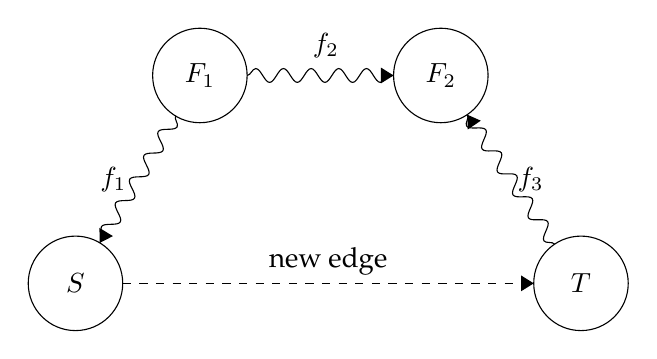
\begin{tikzpicture}[scale=0.2]
\tikzstyle{every node}+=[inner sep=0pt]
\draw [black] (18.1,-36.1) circle (3);
\draw (18.1,-36.1) node {$S$};
\draw [black] (50.2,-36.1) circle (3);
\draw (50.2,-36.1) node {$T$};
\draw [black] (26,-22.9) circle (3);
\draw (26,-22.9) node {$F_1$};
\draw [black] (41.3,-22.9) circle (3);
\draw (41.3,-22.9) node {$F_2$};
\draw [dashed] (21.1,-36.1) -- (47.2,-36.1);
\fill [black] (47.2,-36.1) -- (46.4,-35.6) -- (46.4,-36.6);
\draw (34.15,-35.6) node [above] {new edge};
\draw [decoration=snake,decorate] (24.46,-25.47) -- (19.64,-33.53);
\draw (20.5,-29.5) node {$f_1$};
\fill [black] (19.64,-33.53) -- (20.48,-33.1) -- (19.62,-32.58);
\draw [decoration=snake,decorate] (29,-22.9) -- (38.3,-22.9);
\draw (34,-21) node {$f_2$};
\fill [black] (38.3,-22.9) -- (37.5,-22.4) -- (37.5,-23.4);
\draw [decoration=snake,decorate] (48.52,-33.61) -- (42.98,-25.39);
\draw (47,-29.5) node {$f_3$};
\fill [black] (42.98,-25.39) -- (43.01,-26.33) -- (43.84,-25.77);
\end{tikzpicture}
\end{center}
\caption{Two flip tolerant path.}
\label{figure-two-flip}
\end{figure}

The two flip tolerant path search returns the set of all paths between a given source and sink that have up to two flips (paths with zero or one flip are also accepted).

\paragraph{Path extraction algorithm}
Next, the \textit{path extraction algorithm} th en transforms the output of the two flip path search into the verification set, $\mathcal{Q}' \cup \mathcal{C}'$.
Given a set of two flip tolerant paths from the new edge source to sink, the algorithm outputs a set of pairs to verify.

Let the new edge added to the diagram be $(S, T)$ and the input set of paths, $\mathcal{P}$.
The algorithm processes every two flip tolerant path $p$ in $\mathcal{P}$ case-wise to obtain pairs to add to the output set.
\begin{itemize}
\item In the case where p has two flips, $t_1(p) ; (S, T) ; t_3(p)$ and $t_2(p)$ form a parallel pair.
\item When p has only the first flip (which is to say, the third phase of the path is missing), the parallel paths are $t_1(p) ; (S, T)$ and $t_2(p)$.
\item Similarly when only the second flipping point is present (so that there is no first phase), then the parallel pair is  $(S, T) ; t_3(p)$ and $t_2(p)$.
\item Finally when no flipping points are present, there are two possibilities:
Either $p$ is a path from $S$ to $T$, in which case the parallel paths are simply the edge $(S, T)$ and $p$, or $p$ is a path from $T$ to $S$.
In this case, we have found a cycle, $p ; (S,T)$, to be paired with the identity function.
Like with the na\"{i}ve algorithm, for every node $v$ in the cycle, we add the pair $(v \rightarrow v, 1)$, where $v \rightarrow v$ is the cycle $p ; (S,T)$ written to start and end at $v$.
\end{itemize}

\paragraph{Resolving the Incremental Algorithm}
We conclude our discussion of this incremental algorithm by proving that the result is the same as if we were running the na\"{i}ve baseline algorithm.  This in turn shows that we have found a more efficient algorithm to achieve the same result of providing a set of paths which can be used to check commutativity.

\begin{theorem}
    Perform the two-flip tolerant path search from the source to sink node of the edge that is to be added followed, and on the output, apply the path extraction algorithm. 
    The result is the set $\mathcal{O} = \mathcal{Q}'\cup \mathcal{C}'$ of new parallel pairs with exactly one path passing through the new edge and neither paths containing any cycles, and the set of simple cycles passing through the new edge.
\end{theorem}

\begin{proof}
    Every element in the output of the path extraction algorithm was by construction an element of $\mathcal{O}$. Every cycle in $\mathcal{C}'$ can be expressed as $(S, T) ; p$, and corresponds to the input two flip tolerant path $p$.
    
    It remains to show that every new parallel pair $p$ in $\mathcal{Q}'$ corresponds to a two flip tolerant path.
    Let $\partial(p)^+ = F_1$ and $\partial(p)^{-} = F_2$. 
    Only one path passes through $(S, T)$. Let it be called $p_1$, and the other path, $p_2$.
    The two flip tolerant path from $S$ to $T$ can be constructed as follows: phase 1 is the segment of $p_1$ from $F_1$ to $S$, phase 2 is $p_2$, and phase 3 is the segment of $p_1$ from $T$ to $F_2$.
    Effectively, $F_1$ corresponds to the first flipping point, and $F_2$, to the second.
    It is possible that some of $F_1, F_2, S$ and $T$ coincide (e.g., $p$ starts at $S$, i.e., $F_1 = S$), in which case the corresponding segments between the coinciding nodes can be considered the identity; the resultant path simply has fewer than two flips.
\end{proof}

\paragraph{Analysis}
An upper bound on the number of pairs that this algorithm returns is $O(|V|^{2} 2^{|V|})$, since two flip tolerant paths are an ordering on nodes, each node appearing at most once, followed by a selection of the flip points.
In practice, the algorithm significantly outperforms the na\"{i}ve batch baseline because it looks only at parallel pairs that involve the new edge, which is usually a small subset of all parallel pairs.
Empirical results are presented in Section~\ref{sec:evaluation}.

\subsection{Optimal Batch Solution}

\label{sec:batchBaseline}

Murota's main result~\cite{commutative} solves the batch version of \textsc{verification set}: given an acyclic diagram, it returns the minimal set of equality checks that succeed if and only if the diagram commutes.
Murota describes an algorithm to find the ($|V|^2|E|$ bounded) minimal set of pairs that need be checked.

The approach in this algorithm, at a high level, is to define a function that takes in a subset of pairs and returns the subset of pairs whose equivalence is implied by the equivalence of the pairs in the input set.
Then the algorithm greedily eliminates redundancies until a minimal set is reached.

A bilinking is defined to be a parallel pair that is disjoint but for their terminal nodes. The set of all bilinkings is $\mathcal{R}_0$.
In an acyclic diagram, if all bilinkings are equal, all parallel pairs must also be equal since any given pair can be expressed as a composition of bilinkings.

Define $r_1>r_2$ for bilinkings $r_1$ = $\{p_1,q_1\}$, $r_2$= $\{p_2, q_2)$ $\in$ $\mathcal{R}_0$, if there exists a path $p$ such that $\partial(p) = \partial(r_1)$ and $p$ contains $p_2$.
Define $\langle\rangle$ as:
$\langle r \rangle = \{ s\in \mathcal{R}_0| r>s\}$.

For bilinking $s$, let $F(s)$ be the vector in $\text{GF}(2)^{|E|}$ (where $\text{GF}(2)$ is the Galois field, that is, finite field of two elements) representing the edges present in s (the $n^{\text{th}}$ dimension of $F(s)$ is 1 if the corresponding edge is in $s$, and 0 otherwise).
Let this function be extended to sets, so that for some set of bilinkings $\mathcal{S}$, $F(\mathcal{S}) = \{ F(s) | s\in \mathcal{S} \}$. A notion of linear independence in this vector field exists.

For a set of bilinkings $\mathcal{R}$, the closure function $cl$ is defined as:
$cl(\mathcal{R}) = \{ s\in \mathcal{R}_0| s$ is linearly dependent on $F(\mathcal{R}) \}$.
%
The closure function on $\mathcal{R}$ captures all the pairs that can be made by made by composing or ``gluing together'' the bilinkings in $\mathcal{R}$. 
%
Using these two functions, we define the function $\sigma$ on a set of bilinkings $\mathcal{R}$ as
$\sigma(\mathcal{R}) = \{s \in \mathcal{R}_0 | s\in cl(\mathcal{R}\cap \langle s \rangle) \}$.
This is the function used to capture all the pairs whose equivalence is implied by the equivalence of pairs in $\mathcal{R}$.
%
We use $\sigma$ to iteratively check if a given pair is redundant.
We eliminate Bilinkings until we reach a minimum ``spanning'' subset.

Roughly, the algorithm proceeds by first efficiently finding a \textit{spanning} set of bilinkings (a subset whose verification implies the verification of all bilinkings in the graph).
It does this, starting at every node, by finding the reachable subsection of the graph, and a spanning tree for the subsection.
From each edges in the reachable section that is not a part of the tree, it generates a bilinking using the edge and a path in the tree that is parallel to the edge (\ref{algo-spanning-set}).

\begin{algorithm}[tb]
\label{alg-spanning-set}
\DontPrintSemicolon
\KwResult{Find a spanning set Rs = [$r_1$, ... ,$r_k$].}

Graph existingGraph\;
$R_s$ $\gets$ \{\}\;
\ForEach{node v in V}{
    subgraph $\gets$ existingGraph.extractReachableSection(v)\;
    \tcc{Get the portion of the graph that can be reached starting from v.}
    tree $\gets$ createMinimumSpanningTree(subgraph)\;
    excludedEdges = edges in subgraph - edges in tree\;
    \ForEach{edge e $\in$ excludedEdges}{
        firstPath = tree.findPath(source: e.source, sink: e.sink)\;
        $R_s$.addElement((firstPath, e))\;
    } 
}
\KwRet{$R_s$}\;

\caption{Finding a spanning set of path pairs, as in section ~\ref{sec:batchBaseline}.}\label{algo-spanning-set}
\end{algorithm}

With the spanning set thus initialized, it greedily tries to remove each pair from the spanning set if the set remains spanning even after removing the edge (~\ref{algo-minimal-spanning-set}).

\begin{algorithm}[tb]
\DontPrintSemicolon
\KwResult{Find a minimal spanning set of path pairs (bilinkings) R.}

\SetKwFunction{FSigma}{$\sigma$}
\SetKwProg{Fn}{Function}{:}{}
\Fn{\FSigma{input set S, spanning set Rs}}{
    output $\gets$ \{\}\;
    \For{bilinking $\in$ Rs}{
        smallerPairs $\gets$ allShorterPieces(bilinking)\;
        \tcc{Get fragments that could build up to the bilinking. Corresponds to applying <> function.}
        consideredPieces $\gets$ smallerPairs $\cap$ S \;
        \tcc{Now see if bilinking can be built from these pieces.}
        \tcc{Linear independence is in GF(2) as in algorithm description.}
        \If{linearlyDependent(consideredPieces, bilinking)}{
            output.add(bilinking)\;
        }
    }
    \KwRet{output}
}

R $\gets$ Rs\;
\For{i=1 to K}{
    \If{$r_i \in \sigma$(R-$r_i$)}{
       R $\gets$ R-$r_i$\;
    }
}
\KwRet{R}\;

\caption{Finding a minimal spanning set, as described in section ~\ref{sec:batchBaseline}.}\label{algo-minimal-spanning-set}
\end{algorithm}

The proof of correctness can be found in Murota\cite{commutative}.
The number of checks returned by the algorithm is at worst $O(|V|^2|E|)$. The overall run time of an optimized implementation is $O(|V|^4|E|^2)$.

\section{Solving the Online Addition Problem}

We present a polynomial time solution to the \textsc{verification set problem}.
As in the online baseline algorithm, we do not concern ourselves with parallel pairs where neither or both paths pass through the new edge.

The key observation allowing us to improve on the online baseline is a result of Theorem~\ref{reductionRule} (which we expand on later): for a given source and sink pair, only a single parallel pair needs to be verified.
It is straightforward to see that, should our selected set of pairs and cycles passing through the new edge be verified commutative, the entire diagram must commute.
\ref{algo-online-polynomial} uses this strategy of identifying a parallel pair with exactly one path through the edge for each (source, sink) pair.

\begin{algorithm}[tb]
\DontPrintSemicolon
\KwData{existing graph, new edge.}
\KwResult{Set of parallel pairs to verify.}
\SetKwProg{try}{try}{:}{}
\SetKwProg{catch}{catch}{:}{end}
Graph existingGraph;
Edge newEdge;

parallelPairs $\gets$ \{\}\;
\For{src in existingGraph.Nodes}{
    \For{snk in existingGraph}{
        \try{}{
            \tcc{Use any standard path finding algorithm such as BFS to find a path in the existing graph from the specified source to sink.}
            Path pathWithNewEdge $\gets$ FindPath(
                sourceNode: src,
                sinkNode: newEdge.Source) +\;
            newEdge +\;
            FindPath(
                sourceNode: newEdge.Sink, 
                sinkNode: snk)\;
            \If{src == snk}{
                \tcc{Assign the nullary path from src to snk.}
                pathInOldGraph $\gets$ src\;
            }
            \Else(){
                Path pathInOldGraph $\gets$ FindPath(
                    sourceNode: src, 
                    sinkNode: snk)\;
            }
            parallelPairs.add((pathInOldGraph, pathWithNewEdge))\;
        }
        \catch{PathFindingFailedException}{
           \tcc{No comparable pairs from node src to node snk that need to be checked}
           continue\;
        }
    }
}
\KwRet{parallelPairs}\;
\caption{Online polynomial time algorithm to find parallel pair set.}
\label{algo-online-polynomial}
\end{algorithm}

The \code{try} block is executed at most $O(|V|^2)$ times, which is also the bound on the number of pairs verified.
%
This bound is asymptotically tight, as can be seen in the case where the graph contains $2N$ nodes along $S$ and $T$.
Imagine dividing the nodes into two groups of $N$ nodes each. Every node in group 1 has a forward edge to every node in group 2 and to $S$. $T$ has a forward edge to every node in group 2. In this diagram, when adding edge $(S, T)$, $N^2$ paths need to be verified which is polynomial in the total number of nodes, $2N+2$.

If trying to optimize for path length (say, if composing functions is expensive) then ``find any path'' can be replaced with ``find the shortest path.''

An efficient implementation of the algorithm can run in $O(|V|^2(|V|+|E|))$ time, with space complexity not exceeding the asymptotic $O(|V|^2)$ bound on the output.
In such an implementation, path finding from a given source node to all potential sink nodes could be done in a single $O(|V|+|E|)$ breadth first search.

\subsection{Optimization Step}

In the case where equality checks are very expensive, we begin by finding the minimal set of (source, sink) pairs such that checking for these pairs logically implies having checked the full diagram.

If \ref{algo-online-polynomial} were applied to the diagram shown in Figure~\ref{figure-reduction-rule} there would be redundancies in the output.
It turns out that verifying $g_2=f_2 ; n ; h_2$ is sufficient to ensure the diagram still commutes on the addition of $n$.

\begin{figure}
\begin{center}
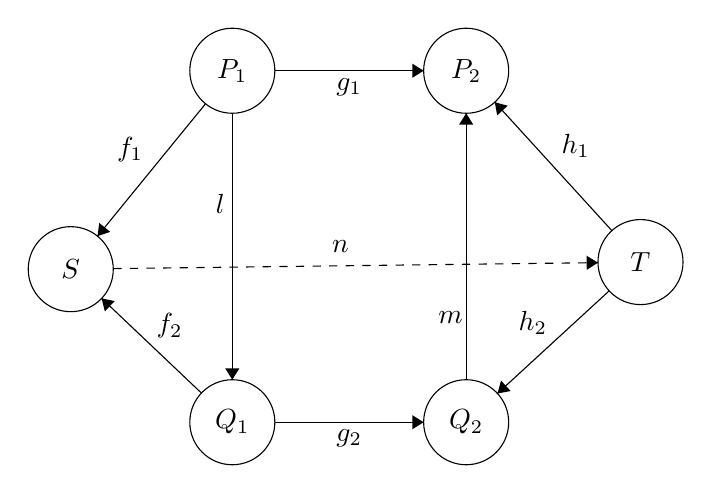
\begin{tikzpicture}[scale=0.18]
\tikzstyle{every node}+=[inner sep=0pt]
\draw [black] (16.6,-34.1) circle (3);
\draw (16.6,-34.1) node {$S$};
\draw [black] (56.8,-33.6) circle (3);
\draw (56.8,-33.6) node {$T$};
\draw [black] (28,-20.1) circle (3);
\draw (28,-20.1) node {$P_1$};
\draw [black] (44.5,-20.1) circle (3);
\draw (44.5,-20.1) node {$P_2$};
\draw [black] (28,-44.9) circle (3);
\draw (28,-44.9) node {$Q_1$};
\draw [black] (44.5,-44.9) circle (3);
\draw (44.5,-44.9) node {$Q_2$};
\draw [black] (31,-20.1) -- (41.5,-20.1);
\fill [black] (41.5,-20.1) -- (40.7,-19.6) -- (40.7,-20.6);
\draw (36.25,-20.6) node [below] {$g_1$};
\draw [black] (26.11,-22.43) -- (18.49,-31.77);
\fill [black] (18.49,-31.77) -- (19.39,-31.47) -- (18.61,-30.84);
\draw (21.74,-25.67) node [left] {$f_1$};
\draw [black] (25.82,-42.84) -- (18.78,-36.16);
\fill [black] (18.78,-36.16) -- (19.01,-37.08) -- (19.7,-36.35);
\draw (23.57,-39.02) node [above] {$f_2$};
\draw [black] (31,-44.9) -- (41.5,-44.9);
\fill [black] (41.5,-44.9) -- (40.7,-44.4) -- (40.7,-45.4);
\draw (36.25,-45.4) node [below] {$g_2$};
\draw [black] (54.59,-35.63) -- (46.71,-42.87);
\fill [black] (46.71,-42.87) -- (47.64,-42.7) -- (46.96,-41.96);
\draw (49.21,-38.76) node [above] {$h_2$};
\draw [black] (54.78,-31.38) -- (46.52,-22.32);
\fill [black] (46.52,-22.32) -- (46.69,-23.25) -- (47.43,-22.57);
\draw (51.19,-25.39) node [right] {$h_1$};
\draw [black] (28,-23.1) -- (28,-41.9);
\fill [black] (28,-41.9) -- (28.5,-41.1) -- (27.5,-41.1);
\draw (27.5,-29.5) node [left] {$l$};
\draw [dashed] (19.6,-34.06) -- (53.8,-33.64);
\fill [black] (53.8,-33.64) -- (52.99,-33.15) -- (53.01,-34.15);
\draw (36.25,-32.5) node [left] {$n$};
\draw [black] (44.5,-41.9) -- (44.5,-23.1);
\fill [black] (44.5,-23.1) -- (44,-23.9) -- (45,-23.9);
\draw (42.5,-37.5) node [right] {$m$};
\end{tikzpicture}
\end{center}
\caption{Reduction rule.
Each arrow represents a path, where $n$ is the new edge being added.
While ~\ref{algo-online-polynomial} returns two pairs for verification, one from $P_1$ to $P_2$ and the other from $Q_1$ to $Q_2$, it actually suffices to just check a pair from $Q_1$ to $Q_2$ as demonstrated in theorem ~\ref{reductionRule}.}
\label{figure-reduction-rule}
\end{figure}

\begin{theorem}
\label{reductionRule}
If parallel paths $g_2 = f_2; n; h_2$ then it must be that $g_1 = f_1; n; h_1$.
\end{theorem} 
% monomorphisms
\begin{proof}
We use the fact that $f_1$=$l; f_2$ and $h_1$=$h_2; m$.
\[g_2 = f_2; n; h_2 \Rightarrow l; g_2 = l; f_2; n ; h_2 \]
\[\Rightarrow l ; g_2 ; m = l ; f_2 ; n ; h_2 ; m \Rightarrow g_1 = f_1 ; n ; h_1\]
%
The proof holds if any of the paths used are the identity, e.g., if $f_1$ is the identity so $S$ and $P_1$ are the same node.
\end{proof}

We conclude that verifying a comparable pair of paths with end points ($P_1$, $P_2$) implies the verification of all path pairs ($Q_1$, $Q_2$) such that $Q_1$ is a successor of $P_1$ and $P_2$ is a successor of $Q_2$. A successor $S$ to node $N$ is any node such that there exists a path from $N$ to $S$. Nodes are also their own successors and predecessors.
The rule effectively places an ordering on the informativeness of path pairs based on their terminal nodes.

Given that a set of path pairs are equal, suppose we attempt to derive the proposition that a different parallel pair of paths is equal with a step-by-step application of inference rules.
 Under the assumption that edges are generic functions, and no other information is available, $\mathcal{F}$ is a semi-group.
 The only inference rules allowed are composition (given that $f_1=f_2$, it must be that $g ; f_1 = g ; f_2$) and replacement of one path by a different, equal path (given $f_1=f_2$ and $g ; f_1 = h ; f_1 $, it must be true that $g ; f_1 = h ; f_2$). Any permutation of the repeated application of these two rules results in the ``reduction rule'' already described; it is therefore the only rule that can be used to reduce the set of path pairs to check.

That is to say, if verifying a comparable pair of paths with end points ($P_1$, $P_2$) implies the verification of a pair with endpoints ($Q_1$, $Q_2$), then it must be that $Q_1$ is a successor of $P_1$ and $P_2$ is a successor of $Q_2$. %TODO proof required?

Using this information it is possible to choose a minimal subset of path pairs to verify, as in \ref{algo-online-minimal}.
%
To summarize this algorithm conceptually, we start by constructing a graph with a node for each possible (source, sink) pair in the graph: each node then represents a possible choice for parallel pair endpoint pairs. Edges are drawn from node ($P_1$, $P_2$) to ($Q_1$, $Q_2$) if $Q_1$ is a successor of $P_1$ and $P_2$ is a successor of $Q_2$. We greedily search for the smallest set of nodes from which the entire graph would be reachable. The idea is to look for ``roots'' in the graph that have to be included in the ultimate verification set because they have no predecessor in the graph and cannot be verified ``through'' the verification of some other pair. Then all the successors whose verification is implied by the roots are eliminated.

\begin{algorithm}[tb]
\DontPrintSemicolon
\KwData{Existing graph, new edge.}
\KwResult{Set of parallel pairs to verify.}
Graph existingGraph\;
Edge (S, T)\;
        
predecessors $\gets$ predecessors of S in existingGraph\;
successors $\gets$ successors of T in existingGraph\;

Graph terminalPairGraph $\gets$ empty \;
\For{q $\in$ successors}{
    \For{p $\in$ predecessors}{
        terminalPairGraph.addNode((q, p))\;
        \For{predecessor $\in$ predecessors of q in existingGraph}{
            \For{successor $\in$ predecessors of p in existingGraph}{
                terminalPairGraph.addEdge((predecessor, successor))\;
            }
        }
    }
}

verificationSet $\gets$ \{\}\;
\While{terminalPairGraph.nodes not empty}{
    currentNode $\gets$ terminalPairGraph.node\;
    \tcp*{an arbitrarily chosen node of terminalPairGraph}
    \While{currentNode has predecessors}{
        currentNode $\gets$ predecessorOfCurrentNode\;
        \tcp*{an arbitrarily chosen predecessor of current Node}
    }
    verificationSet.add(currentNode)\;
    terminalPairGraph.removeAllSuccessors(currentNode)\;
}
\KwRet{verificationSet}\;
\caption{Minimal set finding algorithm.}
\label{algo-online-minimal}
\end{algorithm}

At the end of the greedy graph reduction we are left with the unique set of root nodes.
The only way to reduce the set of parallel pairs is to apply the reduction rule of theorem ~\ref{reductionRule}, but all the ways in which the rule is applicable was already captured in the edges of the graph. The leftover set has no edges and no scope for further reduction.

Also, the verification of the parallel pairs returned in the algorithm implies that the output of the previous algorithm must commute and that the entire diagram must commute.

The run time of the first step is $O(|V|^4)$, and that of the second step is $O(|V|)$, so that the overall bound is $O(|V|^4)$.
Space complexity remains $O(|V|^2)$.

\section{Case Studies}

To demonstrate our algorithms applied to a real world situation, we search for inconsistencies in diagrams of geometry transformations, and in a diagram of the exchange rate between currencies.
Each of these applications use commutative diagrams, and the commutative nature of each is necessary to reason about some form of correctness.
We explore these examples with the intent of showing that the algorithms discussed apply to realistic settings and potentially identify real-world examples of incorrect behavior.

\subsection{Gator}
\label{sec:gator}

Gator is a domain specific language designed around geometry types, which are used to describe properties and transformations of geometric objects~\cite{gator}.  A key feature of Gator is \code{in} expressions, which insert code to automatically transform between two geometry types.  For example, given a point \code{p} represented in 2-dimensional Cartesian coordinates (which has type \code{cart2}), we can transform this point into polar coordinates using the expression \code{p in polar}.  These \code{in} expressions create a structure of commutative diagrams, allowing use as introduced in Section~\ref{introduction}.

Specifically, Gator introduces transformations between \textit{reference frames}, which are the geometry equivalent of transforming between linear algebra basis vectors.  Each edge on our transformation graph is thus a matrix, with composition of edges as matrix multiplication and an oracle checking matrix equality (up to a rounding error $\epsilon$).  

There are several examples of reasonably complicated transformation graphs that we can pick from.  Gator includes graphics examples as part of its examples package, all of which are in the Gator paper; for this evaluation, we looked at the \textit{phong}, \textit{reflection}, and \textit{shadow map} examples.

We implemented a system for interfacing between the optimal set path checker (\ref{algo-online-minimal}) in the open-source implementation of Gator.
The system was tested with intentional bugs, of which it found them all, although no ``real'' bugs were found.  The graphs used were of size 5 or less; for graphs of this size, the checker was able to run in real time with no noticeable loss of frames.  Since the program is running at 60 frames per second, the checker was running at a rate faster than .01 seconds.

\subsection{Currency Graph}
\label{sec:currency}

We imagine a units-of-measure type system as being an interesting application of concurrency graphs; however, to make this more interesting and scale nicely to large graphs with existing data, we focus on the specific unit of currencies.
Consider a diagram with nodes as currencies and a directed edge being the conversion rate from its source node's currency to its sink node's currency.
Since the exchange rate of money from any given base currency to a target currency can be expected to be the same regardless of which intermediate currency transformations are used, this diagram should commute.

Using a web API\footnote{https://exchangeratesapi.io} for currency data, we built the fully connected diagram of exchange rates between 32 currencies on a given day.
To ensure that it indeed commuted, we started with an empty diagram, and added in edges one by one.
Before the addition of each edge, we used the algorithms (\ref{algo-online-polynomial} and ~\ref{algo-online-minimal}, the online polynomial and online minimal set algorithms, respectively) to ensure the addition of a new edge did not introduce inconsistencies in the existing diagram.
If a new edge was problematic, the algorithms returned an example inconsistent pair that would arise from the addition of the edge.
The pair would consist of two currency transformation sequences with the same source currency and ultimate destination currency, but with different effective exchange rates values, as computed by taking the product of all the exchange rates encountered through the chain.

We allowed an ``error tolerance'' so that differences reported would not be the trivial consequences of a floating point error.
However, this relaxation of the equality oracle into imprecision meant that the mathematical reasoning that allow the algorithms to remove redundant path checks no longer applied.
For instance, composing a new function with two approximately equal functions does not lead to equal results, so Theorem~\ref{reductionRule} fails with this approximate equality.
When the algorithms reported no inconsistencies, it was still possible that the graph possessed inconsistencies above the given threshold and did not commute.
Nonetheless, both algorithms were effective in catching inconsistencies. \ref{algo-online-polynomial} started finding inconsistencies at error tolerances to the order of $10^{-3}$, and \ref{algo-online-minimal}, which makes more invalid redundant path check removals, at error tolerances to the order of $10^{-7}$.

Averaging over evaluation for the first 30 days of 2020, building and verifying a diagram to completion (inclusive of the time required by network calls) took 243$\pm$19 seconds using \ref{algo-online-minimal}, and in 133$\pm$13 seconds with \ref{algo-online-polynomial}.
For this large of a graph and data set, these times are reasonable and show these algorithms can be used in a realistic setting.
Finding actual inconsistencies further shows the value of using these algorithms and commutative diagrams in the real world.

\section{Evaluation}
\label{sec:evaluation}
We compare performance of the following path checking algorithms:
(1) the na\"{i}ve baseline,
(2) the less na\"{i}ve two-flip baseline,
(3) the batch baseline,
(4) \ref{algo-online-polynomial}, the non-minimal polynomial-time algorithm, and
(5) \ref{algo-online-minimal}, the minimal set finding algorithm.
The two metrics we evaluate are time for response and size of response set (smaller sets---tighter output results---would mean less calls to the oracle).
We use randomly generated graphs of varying size: given a graph and a new edge, we time how long it takes for an algorithm to return the set of pairs that need to be verified.
All computations were performed on a MacBook Pro 2015, 2.9 GHz dual-core Intel Core i5.

\subsection{Comparison of Algorithm Time Cost}
The average time taken by each algorithm over the course of 10 runs over randomly generated graphs with 9 nodes and 32 edges is listed in Table~\ref{tab:times}.

\begin{table}
    \caption{Computation time for 9-node graph of density 0.4, averaged over ten runs.}
\begin{tabular}{cc}
    \toprule
    Algorithm & Average seconds of computation \\
    \midrule
    Na\"{i}ve baseline & 0.77 \\
    Two Flip tolerant & 0.075 \\
    Batch algorithm & 7.55 \\
    ~\ref{algo-online-polynomial} & 0.0038 \\
    ~\ref{algo-online-minimal} & 0.00086 \\
    \bottomrule
\end{tabular}
\label{tab:times}
\end{table}

\begin{table}
    \caption{Output size for 9 node graph of density 0.4, averaged over ten runs.}
\begin{tabular}{cc}
    \toprule
    Algorithm & Average number of output pairs \\
    \midrule
    Na\"{i}ve baseline & 39754.9 \\
    Two Flip tolerant & 748.9 \\
    Batch algorithm & 23 \\
    ~\ref{algo-online-polynomial} & 78.3 \\
    ~\ref{algo-online-minimal} & 1 \\
    \bottomrule
\end{tabular}
\label{tab:sizes}
\end{table}

\begin{figure}
  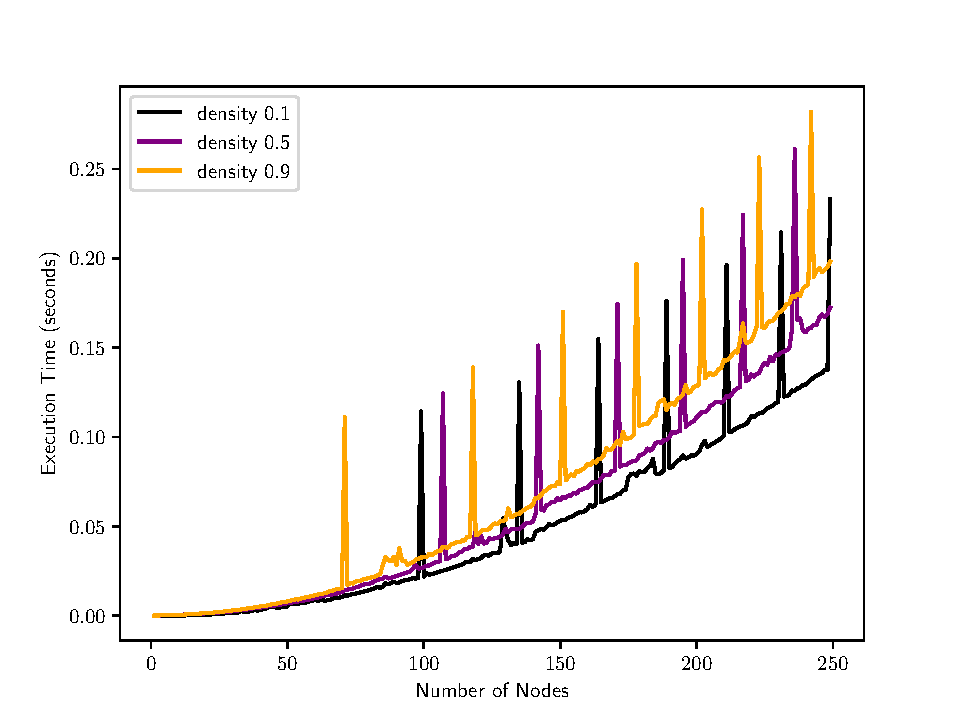
\includegraphics[width=\linewidth,trim=0 0 5 30,clip]{fig/timeVsSize-10-OptimalSet.pdf}
  \caption{~\ref{algo-online-minimal}.}
  \label{fig:sfigOptimalTvsS}
\end{figure}
%
\begin{figure}
  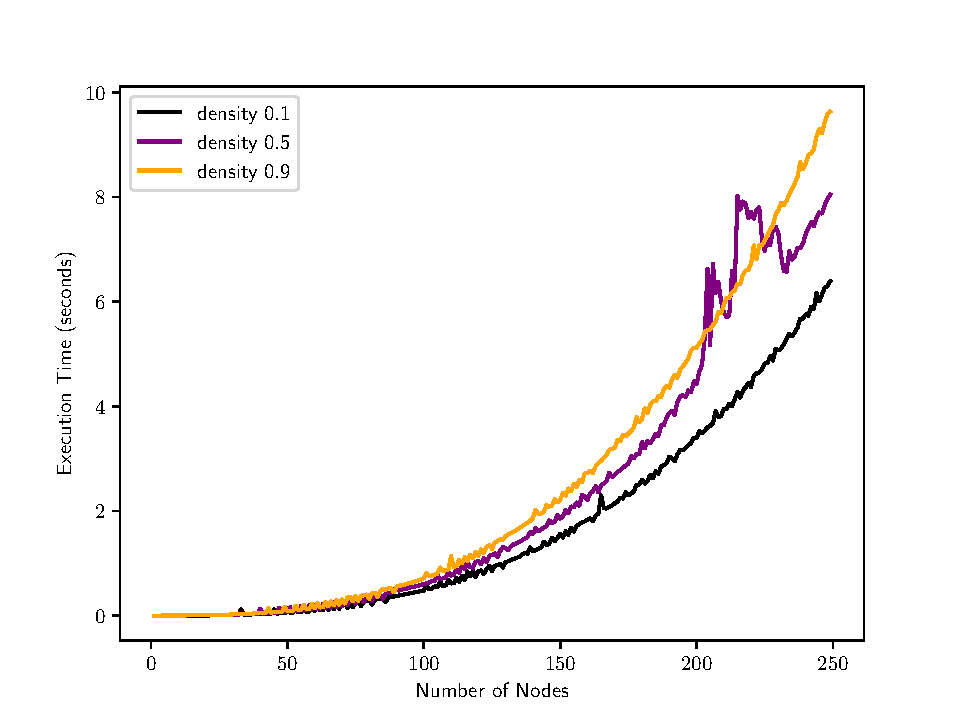
\includegraphics[width=\linewidth,trim=0 0 5 30,clip]{fig/timeVsSize-10-Polynomial.pdf}
  \caption{~\ref{algo-online-polynomial}.}
  \label{fig:sfigPolynomialTvsS}
\end{figure}
%
\begin{figure}
  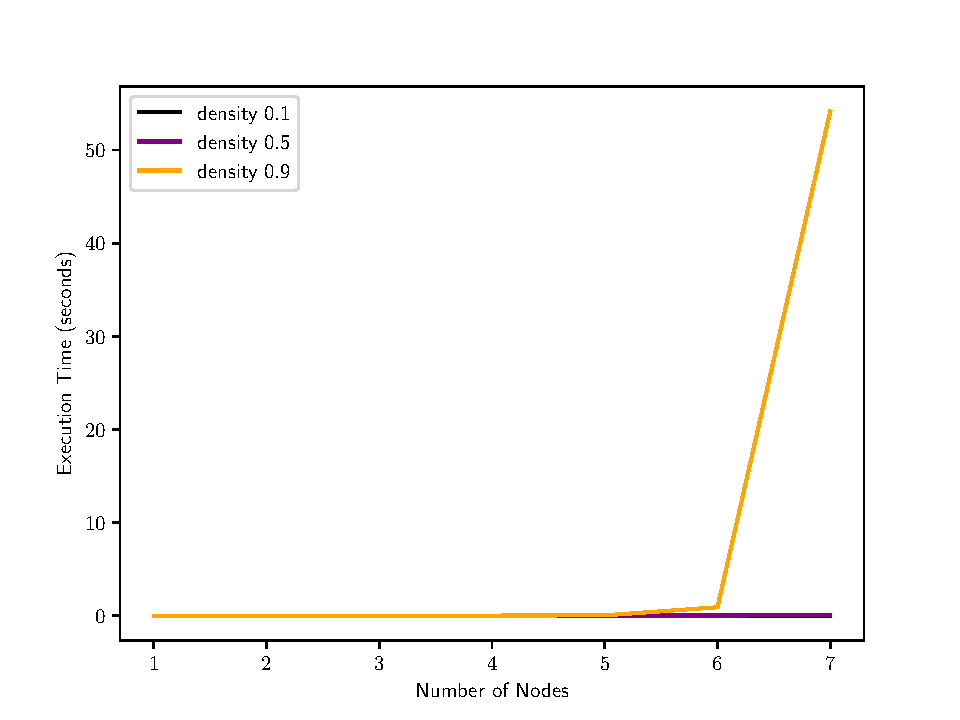
\includegraphics[width=\linewidth,trim=0 0 5 30,clip]{fig/timeVsSize-10-NaiveChecker.pdf}
  \caption{Naive baseline.}
  \label{fig:sfigNaiveTvsS}
\end{figure}
%
\begin{figure}
  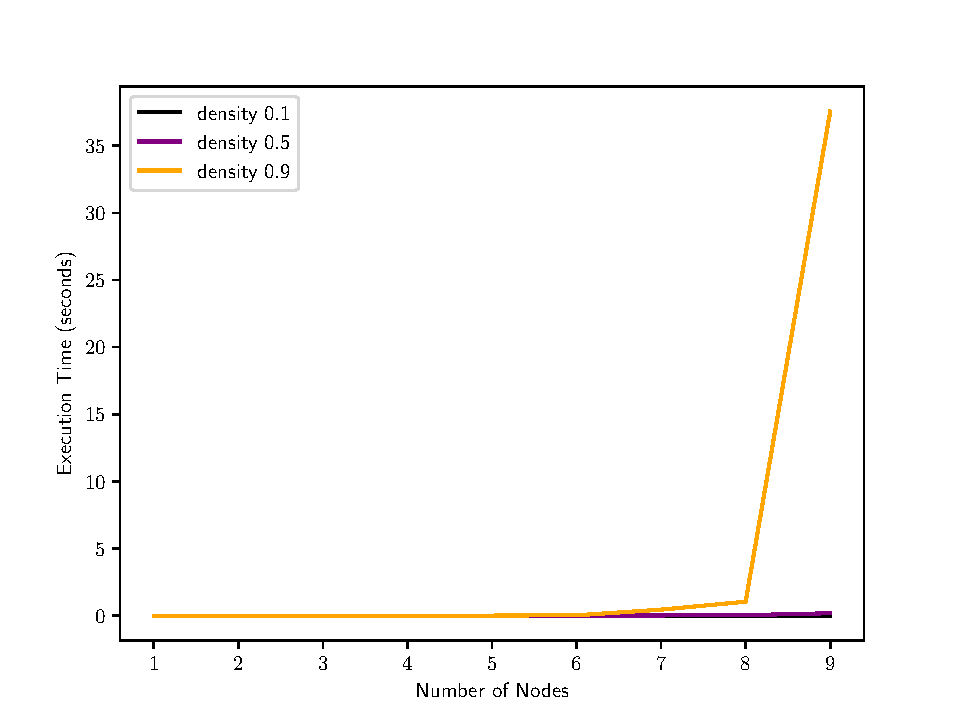
\includegraphics[width=\linewidth,trim=0 0 5 30,clip]{fig/timeVsSize-10-TwoFlipPathChecker.pdf}
  \caption{Two flip tolerant baseline.}
  \label{fig:sfigTwoFlipTvsS}
\end{figure}
%
\begin{figure}
  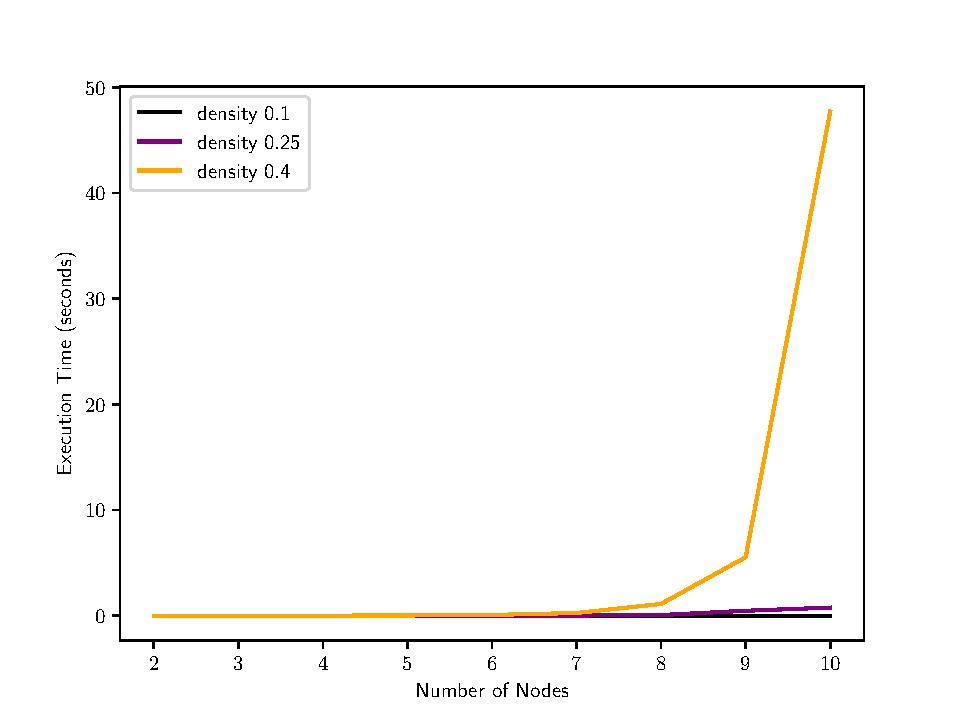
\includegraphics[width=\linewidth,trim=0 0 5 30,clip]{fig/timeVsSize-10-BatchChecker.pdf}
  \caption{Batch algorithm baseline.}
  \label{fig:sfigBatchTvsS}
\end{figure}
\begin{figure}
  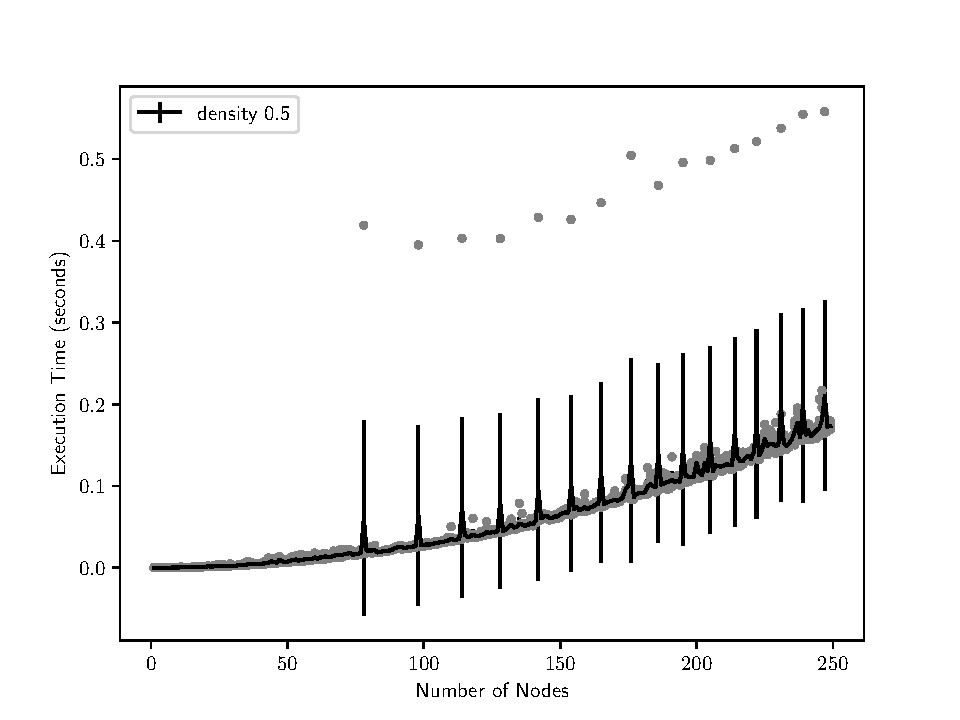
\includegraphics[width=\linewidth]{fig/variance-10-OptimalSet.pdf}
  \caption{~\ref{algo-online-minimal}.}
  \label{fig:sfigOptimalSpread}
  \caption{Spreads of algorithm running times.}
\end{figure}

\begin{figure}
  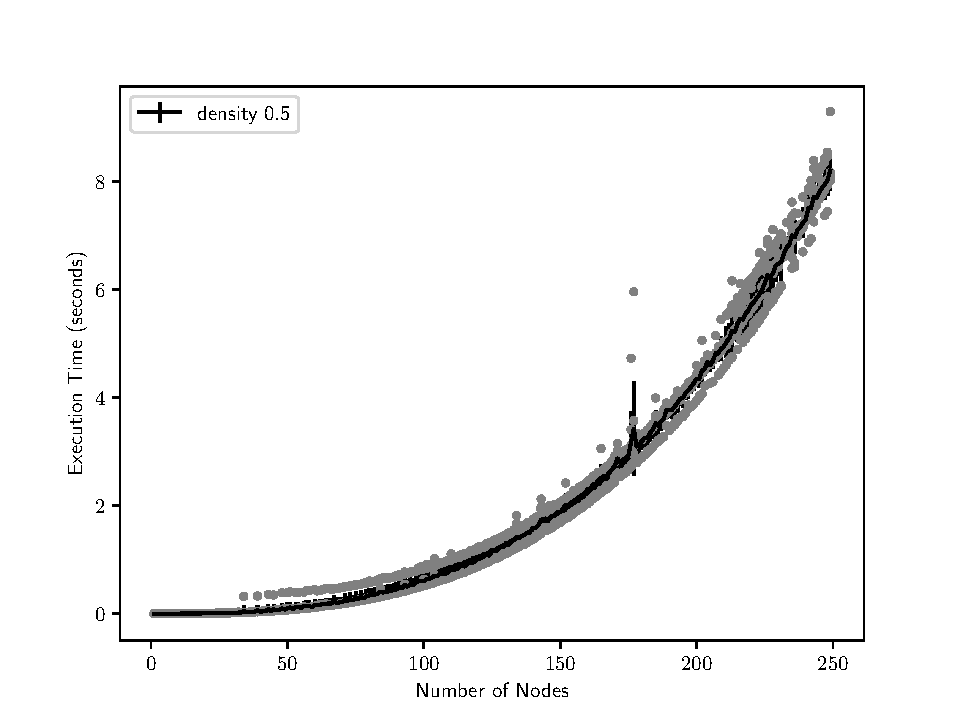
\includegraphics[width=\linewidth]{fig/variance-10-Polynomial.pdf}
  \caption{~\ref{algo-online-polynomial}.}
  \label{fig:sfigPolynomialSpread}
  \caption{Spreads of algorithm running times.}
\end{figure}
    
The na\"{i}ve baseline performs poorly, taking well over a thousand seconds for even small graphs of 10 nodes.
While the batch algorithm improves on this, it still does not scale very well, with computation for a graph with 14 nodes and 0.4 density taking hours.
Our implementation does not memoize the construction of the vector and matrix representation of paths in GF(2); profiling indicates that this construction is a major factor in the high time cost for this algorithm.
\ref{algo-online-polynomial} performs only slightly better than the batch algorithm.
Surprisingly, the optimal set algorithm cuts time cost by several orders of magnitude, and runs in milliseconds for small graphs.
All implementations are sensitive to density, performing better when density is low.
    
\subsection{Scaling of Time with Input Size}

Figure~\ref{fig:timeVsSize} shows that the algorithms' time scales with size, as expected.
\xxx[as]{The plots are weirdly tiny on my machine... any chance your plotting tool can output PDF images?}
Both \ref{algo-online-minimal} and \ref{algo-online-polynomial} exhibit graphs that are polynomial in appearance.
The na\"{i}ve baseline as well as the two flip tolerant baseline display quick growth.
The batch algorithm also grows fast, though not as much as the online checking baselines.

We define density to be the ratio of the number of edges in the graph to the total possible number of edges (which is $|V|^2$, where $|V|$ is the number of nodes).
Run time relates to the density of edges in the input graph.
The degree of the effect differs with the algorithms, as Figure~\ref{fig:timeVsSize} shows.
Generally, denser graphs entail longer computation time.
For the batch algorithm we use lower densities since the input graph must be acyclic. This puts an upper bound on density that approaches 0.5 in large graphs.

\subsection{Variance}
The periodic spikes in Figure ~\ref{fig:sfigOptimalTvsS} are striking. 
We plot the spread of results in Figure~\ref{fig:sfigOptimalSpread} to understand what is happening.
Grey points are the results of evaluation on individual points, and error bars show standard deviation. 
The black curve traces the mean.
We find ~\ref{algo-online-minimal} has outliers about two standard deviation above the mean responsible for the spikes in the average.
The outliers themselves follow a polynomial curve, appearing almost periodically.
We have not yet identified the cause of the behavior.
Figure ~\ref{fig:variance} depicts the situation for ~\ref{algo-online-polynomial}, where no such effect is observed.

\subsection{Size of Output}
Output size is a metric of interest, should the equality checking oracle be expensive.
Table ~\ref{tab:sizes}, summarizes the number of output pairs that the algorithms returned on average over 10 runs, for graphs with 9 nodes and 32 edges.
These results are essentially as expected, although it is interesting to note that Algorithm 3 produces around triple the number of pairs compared to the batch algorithm.
Also note that Algorithm 4 produces the minimal number of paths, showing why it is the minimal set algorithm.

\section{Related Work}

Section ~\ref{sec:batchBaseline} describes Murota's solution to efficiently finding the minimal set of path pairs that need to be compared to check if a given acyclic graph commutes ~\cite{commutative}.
We did not find any other work that solves the question of verifying that diagrams commute.
\balance
However, the question of commuting does come up in programming languages with implicit type conversion.
Gator ~\cite{gator}, as described in Section ~\ref{sec:gator}, supports automatic type conversion between geometry types.
The language implements some restrictions to eliminate obvious cases of non-commuting graphs, but does not verify that defined graphs commute, allowing scope for non-commuting graph definitions.
Frink ~\cite{frink} is a language that supports automatic conversion between units and infinite precision floating point numbers.
It does not appear to support the implicit definition of conversion between units \xxx[AK]{Need to spend some time confirming this} but if extended to do so, would need to contend with the problem of commuting graphs.
The same is true for F\# which has support for units of measure ~\cite{unitsOfMeasure} and Ada's GNAT compiler~\cite{gnat}.

\section{Conclusion}

Being able to verify if diagrams commute allows a compiler to make
deterministic automatic type conversions and can catch inconsistencies of definition in a program with user defined conversions.  In this paper, we have presented verification algorithms that efficiently compute the set of paths that would equal to each other if and only if the diagram would still commute after addition of a new edge.

Integrating conversion consistency checks into widely used languages such as Scala could provide a lot of value to the program.
Since Scala and several other languages provide automatic conversions between types, it seems important to ensure that the choice of which path to take (an apparently arbitrary choice) does not effect the behavior of the program.
Having an algorithm to ensure the commutativity of the resulting diagrams can ensure that behavior is correct and help prevent semantic confusion or errors when using such features.
More engineering work still remains to implement this feature in a language such as Scala, but this paper provides the algorithms necessary to explore a solution.

\chapter{Caiman: DSL for Optimizing Heterogeneous Program Communication (Caiman)}

\section{Introduction}
\label{sec:caimanintro}

Accelerators have become of great interest to the computing community in the last few years \xxx[dg]{TODO: do I need a citation or a few for this?}.  For specific applications or computations, specialized accelerators can provide significant performance improvements.  Using an accelerator, however, can require significant engineering effort and programmer expertise.

A major reason for the complexity of accelerator programming comes from the significant performance concerns that often appear when designing accelerator code.  Intuitively, when an engineer finds that an accelerator is needed for some task, performance is likely a consideration.  Since accelerators are often multithreaded, with specific requirements on data layouts or algorithm design.  These constraints and performance needs have led to years of research to optimize accelerator \emph{kernels} (accelerator--only units of computation) \xxx[dg]{References, though there are so many to pick from}.  However, there is a significant cost in the communication between devices, and specifically when this data communication occurs within the logic of the program.

This cost has been explored in several works in the form of automatic compiler optimizations \xxx[dg]{TODO: add references}, which rely on the compiler to generate communications or kernels based on some heuristic.  Standard GPU compilers have implemented some of these methods \xxx[dg]{TODO: I need to see if I can find a good reference to validate this particular claim}.  Despite these advances, anecdotally programmers are still optimizing performance--critical communication by hand.  This is (at least partially) due to the need for experimentation and profiling in performance--critical code, where a given solution may not perform optimally in all heterogeneous arrangements and even within a given codebase.

As our concrete motivating example of this challenge, graphics programmers often have the need to write very context--aware shaders (the graphics equivalent of kernels), with parts of the shader enabled or disabled depending on static optimization decisions and dynamic information.  To manage this, shader programmers often end up resorting to complicated macros or metaprogramming, where options can be disabled or enabled across code, but also creating a brittle system where adjusting one shader could lead to cascading issues with performance and even program correctness.  Examples of this approach can be clearly seen in the open--source Unreal Engine codebase \xxx[dg](TODO: formally cite these, but just some random examples of this: \footnote{\url{https://github.com/EpicGames/UnrealEngine/blob/release/Engine/Shaders/Private/InstanceCulling/InstanceCullingLoadBalancer.ush}} and \footnote{\url{https://github.com/EpicGames/UnrealEngine/blob/release/Engine/Shaders/Private/HairStrands/HairStrandsClusterCommon.ush}}, which you may or may not be able to see, they just have a bunch of these macros).


We argue, without any meaningful way to prove or refute this claim, that heterogeneous programming is diverse enough and performance--critical enough, that such hand--optimized solutions will continue to be important for kernel and shader engineers.  As a result, we propose a solution that raises the level of abstraction for performance engineering, but engineered so that the layer of abstraction being constructed is both transparent and decomposable.  We start by making more concrete the specific challenges we have observed while hand--optimizing kernels, specifically separating performance and correctness, and managing a combinatorial explosion of kernel interactions.

\subsection{Performance Experimentation}
\label{subsec:separation}

Our running example throughout this paper will be used to illustrate the performance trade--offs inherent in conditional logic and device synchronization.  Specifically, we will be building the \code{select_sum} function, which takes in three arrays `v1`, `v2`, and `v3`, and returns the sum of either `v2` or `v3` depending on the sign of `v1`.

A naive \texttt{Rust} solution for this might look something like the following (for some fixed size of array):
%
\begin{lstlisting}

select_sum(v1 : [i64; N1], v2 : [i64; N2], v3 : [i64; N3]) -> i64 {
  if sum(v1) < 0 {
    sum(v2)
  }
  else {
    sum(v3)
  }
}
\end{lstlisting}
%
Note that, in Rust, an expression without a \code{;} is equivalent to adding a \code{return}, so this code can be read as either returning the sum of \code{v2} or \code{v3}.

We might find that, for large arrays, this code is insufficiently performant in our setting. We might hope to be able to take an approach of the following Rust-like psuedocode, where we simply move our expensive \code{sum} operations onto the GPU:
%
\begin{lstlisting}
select_sum_2(v1 : [i64; N1], v2 : [i64; N2], v3 : [i64; N3]) -> i64 {
  if (sum_gpu(v1) < 0) {
    sum_gpu(v2)
  }
  else {
    sum_gpu(v3)
  }
}
\end{lstlisting}
%
Upon measuring the performance of this solution, however, we may find that this code isn't ``fast enough", even if we are using a highly--optimized GPU implementation of \code{sum}.  If we want to improve the performance of this code further, we have several options.  We could move this entire code onto the GPU (noting, crucially, that the GPU tends to perform poorly with conditions), but another reasonable approach would be to calculate each \code{sum} in advance, to avoid bottlenecking the next GPU calculation behind the CPU condition.  Concretely, in psuedocode, this implementation may look something like:
%
\begin{lstlisting}
select_sum_3(v1 : [i64; N1], v2 : [i64; N2], v3 : [i64; N3]) -> i64 {
  sum1 = sum_gpu(v1);
  sum2 = sum_gpu(v2);
  sum3 = sum_gpu(v3);
  if (sum1 < 0) {
    sum2
  }
  else {
    sum3
  }
}
\end{lstlisting}
%
To complicate this function even more, however, we may have a case where \code{v1} is a smaller array than \code{v2} or \code{v3}, and so sending \code{v1} to the GPU is introducing unnecessary overhead in our computation.  For this special case, we may need to consider the following function variation (even within our same program):
%
\begin{lstlisting}
// For N1 << N2,N3
select_sum_4(v1 : [i64; N1], v2 : [i64; N2], v3 : [i64; N3]) -> i64 {
  if (sum(v1) < 0) {
    sum_gpu(v2)
  }
  else {
    sum_gpu(v3)
  }
}
\end{lstlisting}
%
Note that, in this variation, we may find it optimal to revert to the original idea of having \code{sum_gpu} inside of the condition rather than before, since we are no longer blocking on communication between devices.

It is important to note that every one of these steps we described may depend on measuring performance in a specific setting, with specific array sizes, and even within specific functions.  The particular functions we wrote may or may not be optimal -- an analysis of our timing each variation of this function can be found in~\ref{sec:results} (including blindly moving the entire \code{select_sum} function to the GPU), but we can only show these results for a particular setting.  The takeaway, then, should be that a programmer may need to try each of these variations to find a performant solution, and may need to maintain multiple such functions (such as both \code{select_sum_3} and \code{select_sum_4}) in the same program, despite these functions doing the same computation!

To make matters worse, we are ignoring even more decisions that can be made between these black--box calls to \code{sum_gpu}.  The decision space here will be expanded on in~\ref{subsec:submission}, which will also expand on why these functions may be much harder to write than what we have shown here.  Before we continue, however, we need to explore another problem that arises from maintaining multiple definitions of \code{select_sum}.

\subsection{Combinatoric Explosion}
\label{subsec:combinatoric}

We have shown how to end up with several implementations of \code{select_sum}, where optimal performance may depend on setting-specific experimentation.  Another key aspect to optimizing heterogeneous performance, however, is optimizing for the context of surrounding functions.  This is suggested by our reliance on the condition \code{N1 << N2,N3}, which implies that we ought to be careful about which ``version" of \code{select_sum} to call based on information about the function calling \code{select_sum}.  We can extend this logic the other direction, and find cases where we may prefer one implementation of \code{sum_gpu} over another for a particular choice of \code{select_sum}, which we can name \code{sum_gpu2}.

Concretely, let us define some \code{complicated_function}, where we have three calls (at various points) to \code{select_sum}.  In--code, we can summarize this assumption as follows:
%
\begin{lstlisting}
fn complicated_function(...) {
  select_sum(...);
  // ...
  select_sum(...);
  // ...
  select_sum(...);
}
\end{lstlisting}
%
We may find, however, that \code{complicated_function} is optimized for a particular arrangement of \code{select_sum} implementations; for instance, we might experiment with the following arrangement:
%
\begin{lstlisting}
fn complicated_function(...) {
  select_sum_1(...);
  // ...
  select_sum_3(...);
  // ...
  select_sum_4(...);
}
\end{lstlisting}
%
This sort of experimentation can lead to an explosion of variations to try, where we may find that a given implementation of \code{sum_gpu} is preferable in a particular implementation of \code{select_sum} within this particular \code{complicated_function}, necessitating writing yet another variation of \code{select_sum}, which may require adjusting our other decisions, and so on and so forth.  In this manner, we can quickly end up writing an exponential number of variations of functions, or, practically, write a complex system of macros, comments, and/or implicit dependencies between code variants, with little in the way to help manage this design overhead.

\subsection{Caiman Languages}

To help address these problems with performance experimentation in heterogeneous programming, we introduce the Caiman language.  The core goal of Caiman is to provide a separation between the definition and the implementation of a function, and to allow these function implementations to be used interchangeably in implementation (with some important type--level protections).  In doing so, we make the following contributions in this work:
\begin{itemize}
\item We provide formal guarantees on multiple implementations for the same function \emph{specification}
\item We describe functions that are decomposable, in that a function implementation can be broken apart so that parts can be used by other implementations without duplicating the entire function, all without breaking Caiman's type--level guarantees of matching implementation to definition.
\item We describe and implement a system within Caiman to harness type--directed program synthesis to help reduce the overhead of performance experimentation and to allow transparency into compiler optimizations.
\item We provide a syntax and implementation for both human--writeable Caiman with the above guarantees, and a more precise Caiman IR for analysis and precise operational control.
\item We demonstrate the performance tradeoffs for several WebGPU kernels, and show that a Caiman implementation of these kernels allows a similar performance exploration \xxx[dg]{This last point is still a WIP, and may need to be refined}
\end{itemize}

\section{Related Work}

\paragraph{Scheduling Languages}

The philosophy of Caiman is very similar to that of scheduling languages such as Halide\footnote{\url{https://people.csail.mit.edu/jrk/halide-pldi13.pdf}} and Exo\footnote{\url{https://exo-lang.dev/}} \xxx{TODO: Add proper citations, maybe add Taco or a few others}.  The Caiman strategy of separating performance and implementation concerns is inspired by these sorts of scheduling languages, and indeed the direction for Caiman was initially written to be a scheduling language for heterogeneous interactions.  

Despite this core inspiration, Caiman navigates the specific challenges of heterogeneous programming differently than the scheduling languages we are aware of.   Most notably, Caiman emphasizes design for the combinatoric explosion of kernel design described in~\ref{subsec:combinatoric} and introduces type requirements for the multithreading and condition logic present in heterogeneous decision making.

\paragraph{CUDA, SYCL}

\xxx[dg]{TODO: make this section more detailed}.  There are a bunch of APIs for reasoning about graphics.  These provide various interfaces and mechanisms for heterogeneous implementations, though none has an approach directly comparable to Caiman.  There is an interesting note here to be made about how modern interfaces have focused more on giving control of communication characteristics rather than abstracting it.

\section{Background}
\label{sec:background}

\subsection{Submitting to the GPU}
\label{subsec:submission}

\subsection{Promises}
\label{subsec:promise}

\section{Practical Caiman}
\label{sec:practical}

To explain how Caiman works, we will work through the example shown in the introduction, namely \code{select_sum}.  For this illustration, we will be using code written the user-facing Caiman frontend, as opposed to the Caiman IR described in more detail in~\ref{sec:engineering}.

A Caiman program consists of a series of functions written across several languages: the three \textit{specification} languages and the one \textit{implementation} language.  Informally, a function written in the specification languages describe semantic behaviors of the program, while a function written in the implementation language describes how that program is implemented on the host machine.  This is the core mechanism by which Caiman separates semantic and performance concerns.

Additionally, a particular Caiman specification must deal with one of three distinct properties of the operation it is specifying: the value calculations, the timeline of the events and synchronizations, and manipulations of existing memory.  We give each of these ``kinds" of specification functions a unique name, respectively they are the \textit{value}, \textit{timeline}, and \textit{spatial} specifications.  Any implementation must implement one of each kind of specification, though specifications may be used by multiple implementation functions.

We will start by showing how to implement \code{select_sum} in Caiman's specification language(s), before moving onto describing the choice of implementations Caiman provides.  We will also examine some intuition of why the Caiman typechecker is able to validate an implementation against a given specification, though the formal model and proof will be deferred to section~\ref{sec:formal}.

\subsection{Value Specification}
\label{subsec:value}

Caiman specifications are written as functions with a Rust-like header and declarative bodies.  We emphasize declarative here to mean that declaration order does not matter (as we will see, we are essentially building a dependency graph).  The complete syntax can be summarized as follows:
%
\begin{lstlisting}

// function header, any number of arguments
spec_kind name(arg : type) -> return_type {
  var :- expression
  returns var
}
\end{lstlisting}
%
The specific expressions allowed for each variable declaration depend on the kind of specification.  All specifications, however, share expressions for function calls and ternary conditional expression:
%
\begin{lstlisting}

// function call
fn_name(expr)
// the usual notion of conditions
if cond then expr1 else expr2
\end{lstlisting}
%
The most intuitive Caiman specification to start with is often the \textit{value} function, which describes what calculations are needed for each data value in the program.  We will take a deep dive into describing the value specification for \code{select_sum} before returning to definitions for Caiman's other specification languages in section~\ref{subsec:spec}.  

Our value specification for \code{select_sum} is as follows:
%
\begin{lstlisting}

val select_sum(v1: [i64; N], v2: [i64; N], v3: [i64; N]) -> out: i64 {
    sum1 :- sum(v1)
    sum2 :- sum(v2)
    sum3 :- sum(v3)
    condition :- sum1 < 0
    result :- if condition then sum2 else sum3
    returns result
}
\end{lstlisting}
%
We have written this specification to be more verbose than needed for the sake of providing a more detailed examination of the semantics being used here.  Many of these lines can be condensed or combined (we can just write \code{if sum(v1) < 0 ...}, for example).

Nevertheless, this declaration more-or-less mirrors our naive C code, notably replacing conditional \code{if/else} blocks with the ternary expression \code{if-then-else}.  This distinction is more than just syntactic, Caiman's specification language is designed to have no internal control flow, as hinted at by the syntax.

Additionally, since Caiman's operations are unordered (we can freely move or combine each declaration here without changing the specification meaning), we do not have any requirement that these operations must be executed in the order written.

More precisely, this specification gives us constraints on what values this function must produce, but leaves the details up to the actual implementation.  We can exactly enumerate these requirements as follows:
%
\begin{itemize}
\item \code{v1}, \code{v2}, and \code{v3} are all arrays of type \code{i64}, and this function produces data of type \code{i64} (this is the usual type constraint placed by a function header).
\item The specification variables \code{sum1}, \code{sum2}, and \code{sum3} depend on \code{v1}, \code{v2}, and \code{v3}, respectively.  For each of these, we must apply \code{sum} to produce our respective value.
\item \code{condition} depends on having calculated \code{sum1} already \textit{at some point}, and also have the constant \code{0} as a value.
\item Similarly, \code{result} depends on having calculated \code{condition}, \code{sum1}, and \code{sum2}, thus requiring the calculations of all of their dependencies to have been done.
\item Finally, \code{returns result} informs us that this function will return the \code{result} value.
\end{itemize}
%
Importantly, however, this specification provides formal requirements; as we will shortly in subsection~\ref{subsec:implementation}, Caiman implementations of this specification which do not produce the specified values will fail to typecheck and will be rejected at compile time.  Indeed, we can safely say that each specification variable becomes a type we can refer to while typechecking an implementation function.  We must first take a short diversion into examining Caiman function definitions.

\subsubsection{Function Equivalence}
\label{subsec:equivalence}

We need to take a short dive into how the \code{sum} function is being used in this \code{select_sum} specification.  In Caiman, every function used in a specification must be a \textit{function equivalence class}.  Function equivalence classes consist of a name associated with one or more function definitions (which may be defined in Caiman or externally) that the programmer considers equivalent.

The most immediate use for function classes can be seen with the following definition of \code{sum} that we include in the \code{select_sum} file:
%
\begin{lstlisting}

feq sum {
    extern(cpu) pure sum_cpu([i64; N]) -> i64
    extern(gpu) pure sum_gpu([i64; N]) -> i64
}
\end{lstlisting}
%
Here we are simply saying that we consider the \code{cpu} and \code{gpu} definitions of \code{sum} to be equivalent.  The key reason for introducing these equivalence classes is to allow for multiple implementations of the same function to coexist in the same program, and to allow the user to fearlessly call any particular version in their implementation of some specification.  

Note that \code{select_sum} must also be in such a function equivalence class -- syntactically we name this equivalence class to be the same as our defined value function, in this case just \code{select_sum}.  In this way, Caiman specification functions can call other specification functions without introducing assumptions about the implementations of those functions.  

Importantly, however, Caiman does not attempt to prove this assertion or require any more annotation than exactly the type of the function provided here (the external implementations of \code{sum} could be buggy, and Caiman makes no claim about preventing this).  Similarly, we also make no attempt to verify that an external function implementing a Caiman value specification will match the semantics of that specification, and leave this work to the user.  Stylistically, this means that Caiman's guarantees and utility are strongest when a majority of the code being used in a Caiman program is written in Caiman rather than made external.  

\subsection{Implementation Language}
\label{subsec:implementation}

With our value specification and function equivalence classes in hand, we can now implement a Caiman program for \code{select_sum}.  As a reminder, all the code we have written so far provides typing information for our actual implementation here, and is not compiled into an executable program without this implementation.

Frontend Caiman implementations more-or-less resemble Rust code, with the addition of specifying which particular specification(s) they are implementing.  As noted above, we will only focus on implementing our value specification for now.  Our first implementation of \code{select_sum} is thus as follows:
%
\begin{lstlisting}

fn select_sum_impl(v1: [i64; N], v2: [i64; N], v3: [i64; N]) 
  -> i64 impls select_sum,... {
    if sum_cpu(v1) < 0 { 
        sum_cpu(v2)
    }
    else {
        sum_cpu(v3)
    }
}
\end{lstlisting}
%
This is a valid Caiman implementation of this program, meant to show that in many cases, the programmer can essentially implement code similar to standard languages, where information can mostly be inferred.  For understanding the typechecking work Caiman does on this program, however, it is perhaps more informative to show the explicit Caiman type annotations we can provide for such a program.  When we hand-write these annotations, we produce the following (equivalent) program:
%
\begin{lstlisting}

fn select_sum_impl(
  v1: [i64; N] @ val.v1,
  v2: [i64; N] @ val.v2,
  v3: [i64; N] @ val.v3)
  -> i64 @ val.out
  impls select_sum,... {
    let s1 : i64 @ val.sum1 = sum_cpu(v1);
    let cond : bool @ val.condition = s1 < 0;
    let res : @ val.result = if cond {
        let s2 : i64 @ val.sum2 = sum_cpu(v2);
        s2
    }
    else {
        let s3 : i64 @ val.sum3 = sum_cpu(v3);
        s3
    };
    res
}
\end{lstlisting}
%
Our focus in this rewrite is to expose the (baseline) types used by a Caiman implementation.  Each variable in an implementation has 2 components: an raw datatype and three specification types (we are only showing the value specification type for now for simplicity).  \code{s1}, for example, has a raw datatype of \code{i64}, and a (value) specification type of \code{val.sum1}.

The part of the type \code{node(val.sum1)} has two pieces, \code{val}, and \code{sum1}, with the following meanings:
%
\begin{itemize}
\item \code{val} states that the given type is a part of the value specification this function is implementing, \code{select_sum} in this case
\item \code{sum1} states that we are working with the specific node within our value specification named \code{sum1}.
\end{itemize}
%
Crucially, this is part of the type of the implementation variable as much as the datatype \code{i64}, though the specification type can be erased when compiling Caiman code.  In other words, if we instead wrote the (incorrect) annotation:
%
\begin{lstlisting}

let s1 : i64 @ node(val.sum2) = sum(v1);
\end{lstlisting}
%
Then our code would fail to compile.  Interestingly, this line alone would be enough to fail to compile, as we defined \code{val.sum2:-sum(v2)} in the specification, and since our implementation variable \code{v1} has type \code{input(val.v1)}, the types of \code{v2} and \code{v1} don't ``match up".

An important observation is the type of \code{res}, which is derived from the \code{if-else} condition logic being applied.  In essence, we consider control flow in Caiman's implementation language to have a return type, which can only be a \code{unit} if the associated specification type is a \code{unit}.  We can show that this particular conditional logic works out, because the true case returns a result associated with the value type \code{v2}, while the false case returns a result associated with the value type \code{v3}.  If we swapped the logic to instead produce \code{v3} in the true case and \code{v2} in the false case, we would have a type error.

With our types in hand, we can now rewrite our original code to reorder the sum operations to before the conditional logic, as we originally desired.  The (type-inferred) code in Caiman can be simply written as follows:
%
\begin{lstlisting}

fn select_sum_impl_2(v1, v2, v3) 
  -> i64 impls select_sum,... {
    let s2 = sum_cpu(v2);
    let s3 = sum_cpu(v2);
    if sum_cpu(v1) < 0 {
        s2
    }
    else {
        s3
    }
}
\end{lstlisting}
%
A visibly typed version of this code can be found in the appendix.  This implementation still typechecks and so maintains the value semantics of the \code{select_sum} specification -- a proof of this claim will be given in~\ref{sec:formal}.  Importantly, by providing this function definition, we now have two implementations in the \code{select_sum} function equivalence class -- these can be called elsewhere in Caiman by name with \code{select_sum_impl} or \code{select_sum_impl_2}.

We can now address the notion of actually using function equivalence in our implementation.  Unfortunately, we are not able to yet write our call to \code{sum_gpu} (as alluded to in~\ref{subsec:equivalence}), since we will first need to specify more details about synchronizing to another device (the GPU), and we have so far assumed that the CPU is our local host and so does not need synchronization.

To avoid introducing unnecessary complications to our straightforward equivalence relation, we will instead introduce another implementation of sum on the CPU, extending our equivalence class of \code{sum}:
%
\begin{lstlisting}

feq sum {
    extern(cpu) pure sum_cpu_1([i64; N]) -> i64
    extern(cpu) pure sum_cpu_2([i64; N]) -> i64
    extern(gpu) pure sum_gpu([i64; N]) -> i64
}
\end{lstlisting}
%
This example is clearly synthetic and meant to be illustrative, but even in this case we could imagine a second definition of \code{sum_cpu}: specialized to be multi-threaded while our first definition is single-threaded.

We can freely use either definition within our \code{select_sum} function; for example, we could now write the following code, and the types of each value are identical to what we had before:
%
\begin{lstlisting}

fn select_sum_impl_3(v1: [i64; N], v2: [i64; N], v3: [i64; N]) 
  -> i64 impls select_sum,... {
    if sum_cpu_2(v1) < 0 { 
        sum_cpu_1(v2)
    }
    else {
        sum_cpu_2(v3)
    }
}
\end{lstlisting}
%
This mechanism to freely interchange function definitions is core to Caiman's goal of separating performance decisions and specification, as discussed in Section~\ref{sec:intro}.  Note that here we have introduced yet another definition to the \code{select_sum} function equivalence class to explore swapping out specific definitions.  In this way, we can now avoid the usual combinatorial explosion of logic being checked by relying on the value specification to maintain static consistency.

It is important now to address the limitations of Caiman's function equivalence classes, since they are designed to be very simple (and we hope transparent).  Equivalence classes only apply to exactly function calls, and must either be filled by external functions (which are not checked by Caiman), or by implementations in Caiman.

This means that basic properties like arithmetic or logical equivalence are not reasoned about by Caiman unless explicitly declared.  Concretely, for example, we consider \code{1+1} to be a distinct value from the constant \code{2}.  We will examine potential extensions to Caiman's minimal equivalence system when we discuss future work in Section~\ref{subsec:future}.

\subsection{Timeline and Spatial Specifications}
\label{subsec:spec}

We have thus far focused on a vertical slice through Caiman with the value specification language.  We can now take the intuition and ideas from this explanation to work through Caiman's other two specification languages.  

It is worth noting up--front that Caiman's particular choice of specification languages is not rooted in any sort of experimentation, but instead an intuition of what is needed for the examples we care about -- you could extend the ideas presented here to write an entirely different set of specification languages.  Detailing this more abstract notion of what a specification language is, however, is out of scope of this write--up, and will be left to another, more theoretical paper.

We capture the intent of the value specification language in Caiman as reasoning about the data produced and used by our computation.  When we are working with another device (such as a GPU), however, it is also important to be precise about what threading and memory resources we interact with.  More specifically, we would like to be able to break apart synchronization and memory resources across control flow, in much the same way as the value language allows us to (safely) reuse data and decompose computation on that data into carefully designed pieces.

To achieve this goal, we also introduce the \emph{timeline} and \emph{spatial} specification languages to Caiman.  These languages follow the syntax and declarative approach used by the value specification, but with operations intended to capture the intent of synchronization and memory primitives used when scheduling GPU operations.

A Caiman synchronization mirrors that of the GLSL and WGPU submission processes, described in Section~\ref{subsec:submission}.  This process consists of exactly 3 events, described as a host managing the devices A and B, where device A is providing the data to run and device B is providing the computation and result:
%
\begin{enumerate}
\item The host requests an \emph{encoding} location from device B, which is then given to device A.
\item After device A has finished encoding data, the host \emph{submit}s that device B can begin computation.
\item Once device B has finished the computation, the host allows device A to \emph{synchronize} and access the written data.
\end{enumerate}
%
Caiman employs classic promise semantics for this model, described in~\ref{subsec:promise}.  For the timeline specification, then, we introduce an \code{Event} type, which informally describes a point in time.  Note that we implicitly also introduce subtypes for each step of this process to keep track of the logical flow, where each requirement is maintained structurally as being in dependency order. We also introduce the following three operations to match the stages described:
%
\begin{lstlisting}

// Given an Event, starts an encoding on device B,
//   also produces a 'local' event associated with device A
//   along with a 'remote' event associated with device B
local, remote :- encode_event(e)
// Given a 'remote' event, begins a submission on device B
//   produces a 'submission' event
sub :- submission_event(remote)
// Given a 'submission' and 'local event, 
//  produces a 'synchronization' event on device A
snc :- synchronization_event(local, sub)
\end{lstlisting}
%
We will explore a more detailed example of using the timeline language shortly in Section~\ref{subsec:fullexample}.  First, however, we will summarize the (relatively simple) spatial specification language.

The spatial language is used primarily to specify memory behaviors to help with guarantees related to implemented loops or recursion.  To this end, the spatial language provides a \code{BufferSpace} type, which defines a cluster of memory, along with exactly one operation, used to divide up this buffer space:
%
\begin{lstlisting}

// splits up a given buffer space into n>=1 evenly sized pieces:
separate_buffer_space(buff, n);
// for example, we can split a buffer in half:
buff1, buff2 :- separate_buffer_space(buff, 2);
\end{lstlisting}
%
We will not being working through any examples that define a non-trivial spatial specification, but a recursive example can be found in Appendix \xxx{TODO}.

Having defined our specification functions, we can now fully state that an implementation in Caiman must be associated with exactly one of each kind of specification.  A given implementation need not implement the entire specification of each, so long as the input and output types of that implementation are correct as stated.  Note that this means that a call into a particular Caiman implementation of a function equivalence class may result in a series of calls (some of which may be also used by other Caiman implementations of that specification).

Further, each specification could be implemented by any number of Caiman implementation functions.  Additionally, each specification function has its own equivalence class, which refers to any implementation of that specification (it is rare to use a function equivalence class other than a value specification or for external functions).

Note that a specification can always be trivial (simply taking in a single input and returning it), and so we can syntactically elide a specification in both an implementation header and a variable type.  In these cases, we assume that the type of the implementation variable associated with the missing specification function refers to the trivial specification.
\subsection{Select Sum on the GPU}
\label{subsec:fullexample}

With our timeline and spatial specification functions more carefully defined, we can now construct an implementation of \code{select_sum} that calls into the GPU to calculate either \code{sum(v2)} or \code{sum(v3)} (there are many other variations we can write, but we will start with this approach).  In Rust-like psuedocode, what we are looking to implement resembles the following logic:
%
\begin{lstlisting}

if sum_cpu(v1) < 0 {
    sum_gpu(v2)
} else {
    sum_gpu(v2)
}
\end{lstlisting}
%
First, we reiterate our value specification for ease of readability:
%
\begin{lstlisting}

val select_sum(v1: [i64; N], v2: [i64; N], v3: [i64; N]) -> out: i64 {
    sum1 :- sum(v1)
    sum2 :- sum(v2)
    sum3 :- sum(v3)
    condition :- sum1 < 0
    result :- if condition then sum2 else sum3
    returns result
}
\end{lstlisting}
%
Second, we provide a timeline specification for a \emph{single} synchronization (since we only call the gpu once in each branch, we need only to synchronize once).  As a result, our specification will simply lay out our four stages in sequence:
%
\begin{lstlisting}

tmln single_sync(in : Event) -> out : Event {
    local, remote :- encoding_event(in)
    sub :- submission_event(remote)
    sync :- synchronization_event(local)
    returns sync
}
\end{lstlisting}
%
Third, we provide a (trivial) spatial specification:
%
\begin{lstlisting}

sptl trivial_spatial(b : BufferSpace) -> BufferSpace {
    returns b;
}
\end{lstlisting}
%
Now we can provide an exact implementation for this entire function.  We will write this implementation without explicit value types, though an explicitly typed version can be found in Appendix \xxx{TODO}:
%
\begin{lstlisting}

fn select_sum_impl_gpu(v1: [i64; N], v2: [i64; N], v3: [i64; N]) 
  -> i64 impls select_sum,single_sync,trivial_spatial {
    if sum_cpu(v1) < 0 {
        let enc = encode-begin @ node(tmln.(local, remote)) { v2 } gpu;
        // copy the data from v2 into a gpu variable `v2_gpu`
        encode enc.copy[v2_gpu <- v2];
        // schedule the gpu to write the result 
        //   of sum_gpu(v2) to a variable named s2_gpu
        encode enc.call[s2_gpu <- sum_gpu(v2) @ val.sum2];
        
        // submit the calculation to the gpu
        let fence = submit @ tmln.sub enc
        
        // await the result
        let gpu_data = await @ tmln.sync
        
        // return s2_gpu from the bundled result
        gpu_data.s2_gpu
    }
    else {
        // we apply similar logic here
        let enc = encode-begin @ node(tmln.(local, remote)) { v3 } gpu;
        encode enc.copy[v3_gpu <- v3];
        
        encode enc.call[s3_gpu <- sum_gpu(v3) @ val.sum3];
        let fence = submit @ tmln.sub enc
        let gpu_data = await @ tmln.sync
        
        gpu_data.s3_gpu
        sum_cpu(v3)
    }
}
\end{lstlisting}
%
This implementation more-or-less mirrors the first approach we examined, namely calculating the sum of \code{v2} and \code{v3} inside of the condition.  Now that we have the logic for using the GPU, this approach of first calculating both before the condition will (hopefully) be more immediately appealing.

Interestingly, in this case, we can apply both operations sequentially on the GPU with only a single synchronization, but this requires an unsatisfying black--box solution where we write a \code{sum_2_arrays} type function.  Alternatively, we could write a new timeline specification which allows for two synchronizations, and if our goal were to interleave our encodings and synchronizations, then we would write a new specification.

However, if we are comfortable synchronizing twice, Caiman does provide a clean solution in the form of breaking up our implementation to use the timeline specification twice, without needing to modify any of our specifications:
%
\begin{lstlisting}

fn select_sum_impl_gpu_2(
  v1: [i64; N] @ val.v1,
  v2: [i64; N] @ val.v2,
  v3: [i64; N] @ val.v3) 
  -> i64 @ val.result
  impls select_sum,single_sync,trivial_spatial {
    let enc = encode-begin @ node(tmln.(local, remote)) { v2 } gpu;
    encode enc.copy[v2_gpu <- v2];
    encode enc.call[s2_gpu <- sum_gpu(v2) @ val.sum2];
    let fence = submit @ tmln.sub enc
    let gpu_data = await @ tmln.sync
    let s2 = gpu_data.s2_gpu;
    
    select_sum_impl_gpu_2_inter()
}
fn select_sum_impl_gpu_2_inter(
  v1: [i64; N] @ val.v1, 
  s2: i64 @ val.sum2, 
  v3: [i64; N] @ val.v3)
  -> i64 @ val.result
  impls select_sum,single_sync,trivial_spatial {
    // similar logic to compute s3
    select_sum_impl_gpu_2_ret(v1, s2, s3)
}
fn select_sum_impl_gpu_2_ret(
  v1: [i64; N], 
  s2: i64 @ val.sum2, 
  s3: i64 @ val.sum2) 
  -> i64 @ val.result
  impls select_sum,trivial_timeline,trivial_spatial {
    if sum_cpu(v1) < 0 {
        s2
    }
    else {
        s3
    }
}
\end{lstlisting}
%
This idea of breaking up a function to implement only part of a specification is crucial to using Caiman, as code written in this way can represent unfinished and can avoid duplicating computation.  The reason this code is able to typecheck is precisely because of our explicit annotations on the arguments and return type of each function -- otherwise, the program analysis needed often becomes intractable.  Since Caiman can prove that the type boundaries of each function resolve, we need not worry about the potential complexity introduced between function calls.

Another important observation is that we can use a similar idea to break apart encoding and synchroniziation, allowing a programmer to first encode an operation, then continue doing work on the device, and finally synchronize.  Note that Caiman's restrictions are such that we could not encode an operation and then never synchronize that operation (at least, within a Caiman program where we manipulate the timeline between pieces of control flow), since the types associated with the timeline and spatial specifications must match between each possible branch we could take.

Finally, it is worth acknowledging that this Caiman implementation has become quite complicated even for this simple operation.  These implementations are, by design, rather detailed about each operation that is needed to synchronize information with the GPU (or just any other device).  The intention behind this approach is to allow the user of Caiman to be as precise as possible with defining program implementation.  That being said, having implementations be this dense seemingly defeats the purpose of the guarantees Caiman can make -- if we require the programmer to both write careful specifications and implement those specifications to exacting detail, the effort to maintain this system can quickly get out of hand.

We will address this concern with a core piece of the Caiman design when we discuss in Section~\ref{sec:explication}.  First, however, we need to take a brief detour into examining a formal model for Caiman's type system, to provide formal backing and proof behind the core guarantee of Caiman's implementations actually being checked against the specification.

\section{Formal Model}
\label{sec:formal}

\begin{figure}
\begin{align*}
	\psi &\in \textbf{S}\\
	\phi &\in \textbf{C}\\
	\tau &\in \textbf{T} \\
    d &\defas d_1.d_2 \,|\,
        \tau\,\psi\,\textrm{:-}\, \phi(\psi_1) \,|\,
        \tau\,\psi\,\textrm{:-}\, \textrm{if}\, \psi_1 \,\textrm{then}\, \psi_2 \,\textrm{else}\, \psi_3 
        \\
    p &\defas d.\textrm{returns}\, \psi
\end{align*}
\caption{Hatchling Specification Syntax}
\label{fig:hatchspecsyntax}
\end{figure}

\begin{figure}
\begin{align*}
	\psi&\in \Psi\\
   	\tau&\in \textbf{T} \\
	x&\in \textbf{V}\\
	f&\in \textbf{F}\\
	c&\defas \,c_1 ; c_2 \,|\, 
        x\leftarrow f_\psi(x_1) \,| \tau x \,|\, x\leftarrow\textrm{select}_{\psi} (x_1, x_2, x_3)\\
    p&\defas c;\textrm{return}\, x
\end{align*}
\caption{Hatchling Implementation Syntax}
\label{fig:hatchimplsyntax}
\end{figure}

\xxx[dg]{I include alloc, copy, and ref here because it feels like I need to be clear about the imperative nature of Caiman's implementation, but I actually think these end up being pretty non--interesting.  I feel like the rest of the formalism is enough in retrospect.}

In this section, we will be describing a formal model of the Caiman language. We will use this to prove our assertion that the Caiman typechecker will ensure a given (typed) implementation has the same (observational) semantics as a specification it implements.  We will also be more formally specifying these terms to precisely narrow our claim, and addressing the limitations of this presented approach.

To do this, we will start by describing a subset of the Caiman IR, a language called \textit{Hatchling}.  Hatchling has operations similar to the types and control flow of the Caiman IR, with the goal of describing exactly the type guarantees made by Caiman.

As with the Caiman IR, Hatchling has a specification and an implementation.    Our primary goal will be to setup a proof of the following theorem (although the detailed proof itself will be left to Appendix TODO):
%
\begin{theorem}
Any well-typed Hatchling implementation program with types matching those of a well-typed Hatchling specification program must, for all inputs, either fail to terminate or produce equivalent values as that specification program.
\end{theorem}
%
As an observation about this proof, the term \textit{equivalent outputs} relies on a precise notion of equivalence and values in this context.  Specifically, equivalence is defined exactly as any function that is a member of its function class (as described in subsection~\ref{subsec:equivalence}), while value refers to the series of operations that define some result.  In this sense, we observe that the operation $1+1$ is not considered to be the same value as the constant $2$, unless an equivalence is explicitly stated.

The syntax for each of these Hatchling sub-languages are defined in figures~\ref{fig:hatchspecsyntax} and~\ref{fig:hatchimplsyntax}, respectively.  These syntax rely on external sets of distinct symbols, namely $\mathbf{T}$, $\textbf{S}$, $\textbf{P}$, $\mathbf{V}$, and $\mathbf{F}$.  These sets have no explicit meaning, but intuitively represent the sets of types, specification variables, function classes, implementation variables, and function names, respectively.  Function calls in Hatchling only allow a single argument -- the extension of these proofs to multiple arguments is straightforward but mechanically irksome.  We assume that the set of types $\mathbf{T}$ includes the type $\textrm{unit}$, which we use in the typechecking semantics.  We also assume the set of specification variable symbols $\mathbf{S}$ and the set of function classes $\mathbf{C}$ includes $\mathbf{0}$, a special character that cannot be assigned to and indicates a lack of dependence.

A Hatchling specification program additionally requires 2 contexts, 1 dynamic and 1 static:
\begin{itemize}
\item 
$\Psi:\mathbf{S}\mapsto
\mathbf{T}\bigtimes
\left(\mathbf{C}\bigtimes
\left(\mathbf{S}\bigtimes\mathbf{S}\bigtimes\mathbf{S}\right)
\right)$
, which is dynamic and maps from a specification variable to both its type and its dependencies.  A variable depends either on a function or no function (semantically represented with $\top$), and has exactly 0, 1, or 3 dependencies (0 for an input, 1 for a function call, or 3 for a condition).
\item $\Phi:\mathbf{C}\mapsto\mathbf{T}\bigtimes\mathbf{T}$, which is static and maps from function classes to the input type and the output type of that function.
\end{itemize}

A Hatchling implementation program, on the other hand, similarly requires only 1 dynamic context, but requires 3 constant global contexts (where $\Delta$ and $\Psi$ are built to be derived from the specification associated with the current implementation).  These contexts are as follows:
\begin{itemize}
\item $\Gamma:\mathbf{V}\mapsto\mathbf{T}\bigtimes\left(\mathbf{S}\cup\top\right)$, the sole dynamic context, which maps from an implementation pointer to the type of the data being referred to by that pointer.  This context also includes the associated value if one has been written to the location pointed at by this variable.
\item $\Psi:\mathbf{S}\mapsto
\mathbf{T}\bigtimes
\left(\mathbf{C}\bigtimes
\left(\mathbf{S}\bigtimes\mathbf{S}\bigtimes\mathbf{S}\right)
\right)$
, which must be derived from the result of applying the typechecking rules to a well-typed Hatchling specification.  When typechecking an implementation, however, $\Psi$ is global and constant.
\item $\Phi:\mathbf{C}\mapsto\mathbf{T}\bigtimes\mathbf{T}$, which is the same as with the specification program
\item $\Xi:\mathbf{F}\mapsto\mathbf{C}$, which maps from functions to their owning function class
\end{itemize}

Finally, both Hatchling programs must specify an output type.  For the Hatchling specification program, we denote this as $\tau_\textrm{out}$, while for the Hatchling implementation program, we denote this as $\psi_\textrm{out}$.  Note that we assume that a function being a member of $\Phi$ implies that it is a well--typed function.

\subsection{Typing Semantics}

\begin{figure}
	\begin{mathpar}
   		\inferrule
   		{\Psi,\Psi' |- d_1 \qquad \Psi',\Psi'' |- d_2}
   		{\Psi,\Psi'' |- d_1.d_2}
           
   		\inferrule
   		{\Psi,\Psi' |- d_2 \qquad \Psi',\Psi'' |- d_1}
   		{\Psi,\Psi'' |- d_1.d_2}

		\inferrule
		{\psi\notin\Psi 
        \qquad \Psi(\psi_1)=(\tau_1,\_)
        \qquad \Phi(\phi)=(\tau_1,\tau_2)}
		{\Psi,
        \Psi\sqcup[\psi\mapsto\left(\tau_2,\left(\phi,\left(\psi_1,\mathbf{0},\mathbf{0}\right)\right)\right)]
         |- 
        \tau\,\psi\,\textrm{:-}\, \phi(\psi_1)}

		\inferrule
		{\psi\notin\Psi 
        \qquad \psi_1\in\Psi 
        \qquad \Psi(\psi_2)=(\tau,\_)
        \qquad \Psi(\psi_3)=(\tau,\_)}
		{\Psi,\Psi\sqcup
        [\psi\mapsto\left(\tau,
        \left(\top,
        \left(\psi_1,\psi_2,\psi_3\right)
        \right)
        \right)]
         |- 
        \textrm{if}\, \psi_1 
        \,\textrm{then}\, \psi_2 
        \,\textrm{else}\, \psi_3}
        
   		\inferrule
   		{\Psi,\Psi' |- d \qquad \Psi'(\psi)=(\tau_\textrm{out},\_)}
   		{\Psi,\Psi' |- d.\textrm{return}\,\psi}
	\end{mathpar}
	\caption{Hatchling Specification Typing Judgment}
	\label{fig:spectyping}
\end{figure}

\begin{figure}
	\begin{mathpar}
      	\inferrule
   		{\Gamma(x)=(\tau,\psi)}
        {\Gamma,\Gamma[x/(\tau,\top)]}
        
		\inferrule
		{\Gamma,\Gamma' |- c_1 \qquad \Gamma',\Gamma'' |- c_2}
        {\Gamma,\Gamma'' |- c_1;c_2}
        
        \inferrule
		{
            \Psi(\psi)=(\_,(\phi,(\psi_1,\mathbf{0},\mathbf{0}))) \qquad
            \Xi(f)=\phi \qquad
            \Gamma(x_1)=(\tau,\psi_1) \qquad
        }
        {\Gamma,\Gamma[x/(\tau,\psi)] |- x\leftarrow f_\psi(x_1)}
        
        \inferrule
		{x \notin \Gamma}
        {\Gamma,\Gamma[x/(\tau,\top)] |- \tau x}
        
        \inferrule
        {
            \Gamma(x_i)=(\_,\psi_i) \qquad
            \Psi(\psi)=(\_,(\top,(\psi_1,\psi_2,\psi_3))) \qquad
        }
        {\Gamma,\Gamma[x/(\tau,\psi)] |- x\leftarrow\textrm{select}_{\psi} (x_1, x_2, x_3)}
        
   		\inferrule
   		{\Gamma,\Gamma' |- c, \Gamma'(x)=\psi_\textrm{out}}
        {\Gamma,\Gamma' |- c;\textrm{return}\, x}
	\end{mathpar}
	\caption{Hatchling Implementation Typing Judgment}
	\label{fig:impltyping}
\end{figure}

\subsection{Operational Semantics}

\xxx[dg]{I don't think I actually need operational semantics, since they sort of ``fall out" from the simplified model I decided to go with}

\section{Explication}
\label{sec:explication}

As observed at the end of Section~\ref{sec:practical}, hand--writing Caiman implementations are painful and can practically lead to significant barriers to experimentation.  Specifically, the code itself is dense and can be hard to navigate, but we have found it to be anecdotally difficult to write even with compiler support.  Indeed, it feels as though the work done when implementing a Caiman program is both essentially the same work as writing a Caiman specification and can obscure the performance characteristics being explored.

The entire design of Caiman, however, is such that this task of writing an implementation from a specification can be automated with annotation.  More specifically, we can apply a form of type--directed program synthesis, as seen in several works \xxx[dg]{TODO: get a few citations, this approach has the same notes as several related papers}.

We use explication to describe the task of synthesizing a Caiman implementation from a Caiman specification in the presence of programmer--written implementation requirements.  To make this statement more concrete, we will start by working from example of how this looks in the Caiman frontend.

The author notes that at the time of this writing, the programs shown in this section cannot be written as--is in the Caiman frontend, due entirely to minor missing engineering work on AST transformations.  Approximately equivalent programs can be written explicitly in the Caiman IR (described in ~\ref{subsec:ir}, and the programs are included in Appendix~\xxx{TODO}), but I believe it is important to note this limitation in our actual implementation.  Consequently, more annotations may need to be included in the finished Caiman frontend (to help guide the explicator) than are shown here.

\subsection{Using Explication}

We will start by reiterating our usual value specification for \code{select_sum}:
%
\begin{lstlisting}

val select_sum(v1: [i64; N], v2: [i64; N], v3: [i64; N]) 
  -> [out : i64] {
    sum1 :- sum(v1)
    sum2 :- sum(v2)
    sum3 :- sum(v3)
    condition :- sum1 < 0
    result :- if condition then sum2 else sum3
    returns result
}
\end{lstlisting}
%
Along with a trivial timeline and spatial specification, this is enough to write a fully explicated implementation of \code{select_sum}:
%
\begin{lstlisting}

fn select_sum_expl(
  v1: [i64; N] @ val.v1,
  v2: [i64; N] @ val.v2,
  v3: [i64; N] @ val.v3
) -> i64 : val.out 
  impls select_sum,trivial_time,trivial_space{
  ???
}
\end{lstlisting}
%
With explication, we still need to provide a header (arguments and return types) and the specifications to implement.  When we write \code{???}, however, we are semantically saying that any type-safe code can be inserted to replace this \emph{multi--line hole} in the program.

The Caiman \emph{explicator} can use then types we have given this function to deduce some program that matches these types.  The explicator will not, however, be able to use any other specifications than those given, meaning that it is often the case that no such program exists.  For instance, if we had excluded \code{v1} from our arguments, the \code{select_sum} specification provides no way to construct \code{v1}, and so the explicator would fail to produce a solution.

Importantly, however, the explicator is somewhat possible to control outside of this strictly open \code{???} hole we just defined.  More precisely, we can summarize our explicator requirements with three rules:
%
\begin{enumerate}
\item The synthesized code must typecheck according to our given inputs and outputs, and as defined by our specification.
\item For a fixed implementation and fixed specifications if the explicator produces a program, the explicator must always produce the same program.  That is, the explicator must be deterministic for the resulting program.
\item Any operations provided by the programmer must be used in the order they were written.  Additionally, new operations can only be added where we have a multiline hole (\code{???})
\end{enumerate}
%
The last of these rules, the ordering of operations, is the key piece of the Caiman explicator design that allows for performance manipulation without adjusting the specification (or writing many implementation functions).  We will describe precisely what this rule entails after exposing more of Caiman's implementation in Section~\ref{subsec:control}.  For now, as a concrete example, let us restrict the explicator for \code{select_sum} to ensure that the sum of \code{v2} and \code{v3} must be calculated before the condition:
%
\begin{lstlisting}

fn select_sum_expl_2(
  v1: [i64; N] @ val.v1,
  v2: [i64; N] @ val.v2,
  v3: [i64; N] @ val.v3
) -> i64 : val.out 
  impls select_sum,trivial_time,trivial_space{
  .. = sum(v2);
  .. = sum(v3);
  ???;
}
\end{lstlisting}
%
The key addition to this code is that we have stated that both \code{sum(v2)} and \code{sum(v3)} must be computed and stored (in the unnamed variable \code{..}) before any other computation can be done.  With respect to our explication rules, the order here is important -- by having the \code{???} after these computations, we've required that the explicator can't insert code that we don't expect before these operations.

Of course, the more important reason to introduce to explicator is to help with exploring the more detailed (and complicated) device communication space.  Fortunately, we have introduced enough of Caiman design to use the explicator to help us with writing more complicated with the GPU, taking advantage of the bounds imposed by the timeline specification along with our current value specification.  We first write the timeline specification as shown in Section~\ref{subsec:fullexample} (restated here to help with readability):
%
\begin{lstlisting}

tmln single_sync(in : Event) -> out : Event {
    local, remote :- encoding_event(in)
    sub :- submission_event(remote)
    sync :- synchronization_event(local)
    returns sync
}
\end{lstlisting}
%
And now we can write our implementation, providing some structure to ensure we achieve our desired behavior of only encoding and syncing with the GPU once depending on our condition:
%
\begin{lstlisting}

fn select_sum_expl_gpu(
  v1: [i64; N] @ val.v1, 
  v2: [i64; N] @ [val.v2, tmln.in], 
  v3: [i64; N] @ [val.v3, tmln.in]) 
  -> i64 @ [val.out, tlmn.out] 
  impls select_sum,single_sync,trivial_spatial {
    if sum(v1) < 0 {
        ???
    }
    else {
        ???
    } 
}
\end{lstlisting}
%
Since we have only allowed work within each branch of the condition, we can be confident that we will compute \code{v2} and \code{v3} respectively.  Additionally, our restriction that our inputs are associated with \code{tmln.in} and our outputs are associated with \code{tmln.out} means that we must have synced with a device to produce these results.  Strictly speaking, Caiman does not guarantee which device is used, as in our current explicator implementation we only allow synchronization with the GPU; this would, however, not be difficult to change.

A slightly more interesting observation is that eliding the condition here (\code{if sum(v1) < 0}) will result in the same program in this particular case, due to the way we have written our timeline specification.  By both specifying we can only synchronize with the GPU once, only providing a definition for a single \code{sum} kernel, and requiring that we produce a result with \code{tmln.out}, we have restricted our implementation sufficiently that there is only one viable solution.  This sort of constraint can be difficult to observe in practice, however, motivating the use of partial implementations such as the condition shown here in cases where the programmer explicitly desires this structure.

The other important consequence of observing the extent by which Caiman specifications restrict implementation is how many specification and partial implementations arrangements result in an overconstrained and unsolvable system.  This can be seen as advantageous, in that attempting an explication can save a programmer significant effort after reaching an impossible--to--proceed state, but the explicator may instead time out without resolution.  Consequently, transparent messaging is important when working with the explicator, both information about what the explicator was able to produce and where it may have become stuck.  The specific engineering around the explicator and user messaging will be explored in Section~\ref{subsec:compilation}.

For the remainder of this section, we will examine the algorithm used by the Caiman explicator.  Before we can do so, however, we need to expose a lower--level representation of Caiman code, the Caiman IR.

\subsection{Caiman IR}
\label{subsec:ir}

So far, we have focused on the human--usable Caiman frontend, used to illustrate the intention of Caiman design and how this design can be realistically used by a programmer.  When dealing with explication and precise performance characterization, however, it is helpful to expose the precise operations evaluated by Caiman in the form of an exact (dense) intermediate representation.  It is worth noting that the Caiman IR is implemented to be interfaced with directly as needed, though ideally a programmer is able to avoid writing such code explicitly.

Caiman IR is written to be syntactically distinct from the frontend to avoid confusion, and has the following properties meant for analysis:
%
\begin{itemize}
\item A Caiman IR program consists of ``funclets" (similar to basic blocks with named inputs and outputs) to contain operations.  There is no control flow in a funclet, and calls between funclets use continuation passing style \xxx{TODO: ref CPS}.
\item Caiman IR uses Static Single Assignment (SSA) \xxx{TODO: ref}, so each name is unique.  For ease of use, we allow \code{\%_} to be used to represent an anonymous variable (which may still be used by the Caiman explicator).
\item Each operation consists of exactly instruction, and produces either nothing or exactly one result.
\item There are minimal operations in Caiman IR (around 30 with our current implementation), with much of the work being done on external operations.
\end{itemize}
%
These properties are why we need to expose Caiman IR for explication.  Specifically, we need to have a sense of Caiman's internal representation to describe explication concretely.  

For the sake of examples, we will expose 7 operations in a Caiman IR implementation function.  Note that there are distinct operations used in the Caiman IR specifications; these are similar enough to the specifications we have already seen that we will not need to show them here (complete Caiman IR examples can be found in Appendix \xxx{TODO}).  For these operations we are exposing, we are ignoring some implementation cruft in the Caiman IR that is unnecessary for understanding the programs, but will appear in the examples provided.  These operations are described as follows:
%
\begin{itemize}
\item \code{alloc-temporary}, which takes in a place (local, cpu, or gpu) and an exposed datatype (such as \code{i64}), and produces a memory location that can be written to.  Caiman IR does not distinguish between stack and heap allocations.  We expose \code{alloc-temporary} as the only allocation mechanism for simplicity, in cases where we need to return the reference rather than just data, we would use another operation instead.
\item \code{read-ref}, which takes in a reference and returns the data referred to by this reference.
\item \code{begin-encoding}, which takes in a place to encode to (cpu or gpu), an associated timeline specification node, and a list of memory locations to request for encoding, then returns a reference to an encoder.
\item \code{local-do/encode-do}, which takes in an external function (such a \code{sum}), a specification node to match with, arguments to the function, and, in the case of \code{encode-copy}, an encoder to operate with.  With this, this operation writes the result of this function to call to a given allocation slot.  Returns nothing.
\item \code{local-copy/encode-copy}, which takes in a source reference and a destination reference (and an encoder in the case of encode--copy), and copies the data referred to by the source to the location referred to by the destination.  Returns nothing.
\item \code{submit}, which takes in an encoder and a timeline specification node to associate with, and submits the encoded jobs to the associated device.  Returns a reference to the resulting fence to later synchronize on.
\item \code{sync-fence}, which takes in a fence and a timeline specification node, and requires synchronizing on that fence before continuing.  Returns nothing.
\end{itemize}
%
Additionally, the Caiman IR defines several possible tail edges for funclet implementations to provide type information and to manage continuations when interacting with control flow.  We will expose 2 of these tail edges, though to avoid excessive detail, we will defer discussion of the continuation logic to Section~\ref{sec:engineering}:
%
\begin{itemize}
\item \code{return} takes a single argument as the value to be returned from this funclet.  Note that, to pass typechecking, the given data must match all of the specifications required by the return type of this funclet.
\item \code{schedule-select} takes in a \code{i32} or \code{i64} value to use to select a function, an ordered array of funclets (with matching arguments and return types) to select, the specification node(s) this selection is associated with, the arguments to the selected function, and a function to join with per continuation--passing style.  The return type of each selected funclet must match arguments of the joined funclet, and the return type of the join funclet must match the return type of this funclet.
\end{itemize}
%
\subsubsection{Worked Example}

With our definitions in mind, we can now show an example assembly implementation for \code{select_sum}.  We will be showing the hand-translated equivalent to the implementation first shown in~\ref{sec:practical}:
%
\begin{lstlisting}

fn select_sum_impl(v1: [i64; N], v2: [i64; N], v3: [i64; N]) 
  -> i64 impls select_sum,... {
    if sum_cpu(v1) < 0 { 
        sum_cpu(v2)
    }
    else {
        sum_cpu(v3)
    }
}
\end{lstlisting}
%
Since we will need to refer to specification nodes for our assembly implementation substantially, we will also rewrite our usual value specification to make these names concrete:
%
\begin{lstlisting}

val select_sum(v1: [i64; N], v2: [i64; N], v3: [i64; N]) 
  -> [out : i64] {
    sum1 :- sum(v1)
    sum2 :- sum(v2)
    sum3 :- sum(v3)
    condition :- sum1 < 0
    result :- if condition then sum2 else sum3
    returns result
}
\end{lstlisting}
%
Since Caiman IR funclets do not have control flow, we must start by defining a function to compute the condition of the \code{if} statement, and then calling funclets that represent the left and right branches with \code{schedule-select}.  Note that we will be using \code{...} to indicate elided syntax cruft that is irrelevant for this example (as opposed to the \code{???} or \code{?} Caiman syntax for an explication hole):
%
\begin{lstlisting}

schedule[...] %select_sum_main<...>
(%v1 : val.%v1 ..., 
 %v2 : val.%v2 ..., 
 %v3 : val.%v3 ...) 
  -> [%out : val.%out ...] {
    // We are eliding irrelevent allocation details
    // Note we allocate locally rather than on the CPU
    //   in doing so, we can avoid synchronizing on the CPU
    //   which may, in general, be another device
    %ref = alloc-temporary local [...] i64;
    
    // write the result of sum(v1) to ref
    local-do-external %sum val.%sum1(%v1) -> %ref;
    
    // read the result into a local variable
    %sum1 = read-ref i64 %ref;
    
    // We will not show how to get the constant 0
    %zero = ...
    
    // write the result of sum1 < 0 to ref
    local-do-external %lt val.%condition(%sum1, %zero) -> %ref;
    
    // read the result into a local variable
    %cond = read-ref i64 %ref;
    
    // we will not show how we are computing join
    %join = ...
    
    // we will be writing the left and right branches shortly
    // note that we must pass %v2 and %v3 to both
    //   since their input types must "match up"
    // note also that we specify %result rather than %out
    //   since the if/then/else in the specification gives %result
    schedule-select %cond [%select-sum-left, %select-sum-right]
      [val.%result, ...] (%v2, %v3) %join;
}
\end{lstlisting}

Syntactically, it is worth noting that we use \% to indicate a Caiman IR defined variable to help with distinguishing from the frontend and to visually distinguish between operations and variables.  We have been careful to note each detail we are eliding, which are either irrelevant or out of scope for this writing -- most notably the calculation of the join operation, the complete type syntax Caiman IR uses, and additional qualifiers needed for allocation.

This code provides a precise representation of the line-by-line operations required for Caiman's analysis and compilation.  Fortunately, the left and right branches of this condition are simpler than this selection program, at least when we run locally:
%
\begin{lstlisting}

schedule[...] %select_sum_left<...>
(%v2 : val.%v2 ..., 
 %v3 : val.%v3 ...) 
  -> [%out : val.%sum2 ...] {
    %ref = alloc-temporary local [...] i64;
    local-do-external %sum val.%sum2(%v2) -> %ref;
    %res = read-ref i64 %ref;
    return %res;
}

schedule[...] %select_sum_right<...>
(%v2 : val.%v2 ..., 
 %v3 : val.%v3 ...) 
  -> [%out : val.%sum3 ...] {
    %ref = alloc-temporary local [...] i64;
    local-do-external %sum val.%sum3(%v3) -> %ref;
    %res = read-ref i64 %ref;
    return %res;
}
\end{lstlisting}
%
These funclets are nearly identical, except for their return type and computation.  We observe that these functions can be used in selection because we have annotated our selection with \code{val.}\%\code{result}, which is sufficient for the typechecker to agree so long as each branch return type ``lines up" with its respective branch in the specification.  Finally, then, we can write the (trivial) funclet to join the original selection:
%
\begin{lstlisting}

schedule[...] %select_sum_ret<...>
(%v1 : val.%v1 ..., 
 %v2 : val.%v2 ..., 
 %v3 : val.%v3 ...) 
  -> [%out : val.%out ...] {
    return %res;
}
\end{lstlisting}
%
Morally, this function mirrors the return that we have in the specification, and explicitly provides the connection between \code{val.}\%\code{result} and \code{val.}\%\code{out}.

\subsubsection{Extending to the GPU}
\label{subsec:gpuir}

With our overview of Caiman IR in hand, we will briefly examine how to interface with the GPU.  This code will be quite similar to our high--level Caiman frontend example shown in~\ref{subsec:fullexample}, but is useful for demonstrating our introduced Caiman IR GPU operations.

Specifically, we can modify our funclet \code{select_sum_left}, (note that similarly we could modify \code{select_sum_right}).  Concretely, we will be implementing the usual single--synchronization timeline function:
%
\begin{lstlisting}

tmln single_sync(in : Event) -> out : Event {
    local, remote :- encoding_event(in)
    sub :- submission_event(remote)
    sync :- synchronization_event(local)
    returns sync
}
\end{lstlisting}
%
Concretely, our Caiman IR implementation is as follows:
%
\begin{lstlisting}

schedule[...] %select_sum_left<...>
(%v2 : val.%v2 time.%in ..., 
 %v3 : val.%v3 time.%in ...) 
  -> [%out : val.%sum2 time.%out ...] {
    // Create a reference to the gpu memory 
    //   we will be able to write to
    // Note that this memory is not available 
    //   until we have an encoding
    %v2_gpu = alloc-temporary gpu [...] [i64; N];
    %res_gpu = alloc-temporary gpu [...] i64;
    %res_local = alloc-temporary local [...] i64;
    
    // Begin an encoding with references 
    //   for our input (v2_gpu) and output (res_gpu)
    %enc = begin-encoding gpu time.%enc [%v2_gpu, %res_gpu] [];
    
    // We can now write to this memory location
    // Note that this copy does not have 
    //   an associated specification operation
    // In other words, if we had some 
    //   other mechanism to have a value
    //   of type v2 in the right place at the 
    //   right time, we could use that instead
    encode-copy %enc %v2 -> %v2_gpu;
    
    // Encode running the `sum` operation after our copy
    // Writes the result to our earlier encoded memory location
    encode-do %enc %sum_gpu val.%sum2(%v2_gpu) -> %res_gpu;
    
    // Submite the operations and recover a fence
    %fnc = submit %enc time.%sub;
    
    // Synchronize locally against the GPU result
    sync-fence %fnc time.%snc;
    
    // Copy the result back to the local allocation
    // We can do this because we have synchronized
    local-copy %res_gpu -> %res_local;
    %res = read-ref i64 %res_local;
    return %res;
}
\end{lstlisting}
%
In this GPU implementation, we hint at type rules to manage memory allocations when encoding, submitting, and synchronizing.  We will include engineering for these interactions in our explicator implementation, but the type--safety guarantees we would intuitively aim for are left to a future work.

\subsection{Explication of Caiman IR}

\xxx[dg]{Note that our actual explicator implementation for this example at this time of writing is missing a couple of implementation details that are described here.  Specifically \code{???} is not carefully tested, and \code{begin_encoding} is not fully implemented}.

With our more-exact representation of Caiman IR in hand, we can provide a precise definition of Caiman's explication syntax.  Caiman allows exactly two synctatic ``holes", defined as follows:
%
\begin{itemize}
\item \code{?}, which indicates a specific component of a specific operation can be explicated
\item \code{???}, which indicates that the explicator can introduce any number of operations (including introducing new funclets for control flow).
\end{itemize}
%
As before, \code{???} also means that the explicator can only introduce operations within the block outlined by operations surrounding this multi--line hole.  We will summarize these requirements through a partial explication for \code{select_sum_main}:
%
\begin{lstlisting}

schedule[...] %select_sum_main<...>
(%v1 : val.%v1 ..., 
 %v2 : val.%v2 ..., 
 %v3 : val.%v3 ...) 
  -> [%out : val.%out ...] {
    // do any setup needed to work out the condition
    ???;
  
    // require that we use exactly %lt, 
    // and that we must work out val.%condition in this funclet
    // note that we explicitly state 
    //  a requirement of two arguments here
    //  though we do not say what these arguments are
    local-do-external %lt val.%condition(?, ?) -> ?;
    
    // do any setup neeeded for the schedule-select
    ???;
    
    // We must branch into the funclets 
    //   select-sum-left and select-sum-right
    // We also must have this select be associated with val.%result
    // otherwise, the explicator may do as it would please
    schedule-select ? [%select-sum-left, %select-sum-right]
      [val.%result, ...] (?, ?) ?;
}
\end{lstlisting}
%
There are many ways we could write this partial implementation such that no solution exists, including providing the incorrect number of required arguments to \%\code{lt}.  Given how large the space of impossibilities are, the explicator makes no attempt to prove that no program solution exists, but instead will fail to terminate.  Additionally, the explicator does not fully typecheck existing code, and so only ensures that the code produced is type--safe assuming a correctly typed partial implementation.  Details of how our engineered explicator with the Caiman typechecker are expanded more in~\ref{subsec:compilation}.

The Caiman explicator also works with the operations needed to encode and synchronize on another device.  For example, the following funclet header is sufficient to produce the implementation described in~\ref{subsec:gpuir}:
%
\begin{lstlisting}
schedule[...] %select_sum_left<...>
(%v2 : val.%v2 time.%in ..., 
 %v3 : val.%v3 time.%in ...) 
  -> [%out : val.%sum2 time.%out ...] {
    ???;
    encode-do ? %sum_gpu val.%sum2(?) -> ?;
    ???;
}
\end{lstlisting}
%
Note that we must include this specific \code{encode-do} to be sure that we are actually running the operation on the GPU.  Otherwise, the explicator could very reasonably choose to run this operation locally, and simply apply a no--op to the GPU to progress to \code{time.}\%\code{out}.  In other words, the particular operation we expect to apply to compute \code{sum2} would otherwise be left as an implementation detail of the explicator.

\subsection{Core Algorithm}

We now have the context to define an explication algorithm.  Generally speaking, our approach will be to make arbitrary (type--safe) decisions for the first node of the funclet, recurse to see if we produce a valid explication result, and then try the next decision we could make.  Conceptually this algorithm resembles a depth first search through the decisions we could make, and if we find a type--safe result, we simply return this result.

\begin{algorithm}[tb]
\DontPrintSemicolon
\KwData{A list of solved Caiman IR Nodes, a set of nodes we have yet to use, and the current Caiman IR funclet.}
\KwResult{Either (a list of explicated nodes, a list of requests for multi--line explication to be done) or \textbf{NONE} if no solution was found}
[Node] solvedNodes\;
\{Node\} unusedNodes\;
Funclet funclet\;

\Begin{

    index $\gets$ \textit{Length}(filledNodes)\;
    nodes $\gets$ \textit{Nodes}(funclet)\;
    \tcp*{base case (we assume 0-indexing)}
    \If{index $=$ Length(nodes)} {
        \KwRet{TailEdgeExplication(filledNodes, unusedNodes, funclet)}\;
    }

    currentNode $\gets$ nodes[index]\;
    
    \If{IsMultilineHole(currentNode)}{
        result $\gets$ \textit{NodeExplication}(filledNodes + currentNode, unusedNodes, funclet)\;
        \If{IsNone(result)}{
            \KwRet{\textbf{NONE}}
        }
        \Else {
            (explicated, requests) $\gets$ result\;
            \KwRet{(requests + explicated, [])}
        }
    }
    
    \For{solution $\in$ ValidSolutions(nodes, index, funclet)}{
        usedNodes $\gets$ \textit{GetUsedNodes}(solution)\;
        solutionRequests $\gets$ \textit{GetMultilineRequests}(solution, solvedNodes)\;
        
\tcp*{copy nodes, with our solution added}
        newNodes $\gets$ nodes + solution\;
        newUnusedNodes $\gets$ (unusedNodes $\cup$ currentNode) $\setminus$ usedNodes\;
        result $\gets$ \textit{NodeExplication}(newNodes, unusedNodes, funclet)\;
        \If{~IsNone(result)}{
            (explicated, requests) $\gets$ result\;
            \tcp*{prepend our solution and requests}
            \KwRet{(solution + explicated, solutionRequests + requests)}
        }
    }
    \KwRet{\textbf{NONE}}
}
\caption{NodeExplication}
\label{algo-explication-node}
\end{algorithm}

The algorithm used to explicate a node of a Caiman IR funclet is more precisely described in Algorithm~\ref{algo-explication-node}.  We start this recursion with an empty list of solved nodes, all of our funclet inputs in the set of unused nodes, and our funclet definition.  Note that the funclet definition we provide is intended as a static reference, and is not modified as we recurse.  

If \textit{NodeExplication} returns \textbf{NONE}, then no solution was found.  If this function returns a pair that includes a list of any requests for multiline explication, then we continue the recursion with the next solution for the first node.  Otherwise, we accept the valid explication solution as the list of explicated nodes (along with an explicated tailedge, which is elided in the result for readability).

\textit{unusedNodes} deserves special mention, as this set holds information about all programmer--given nodes (starting with the funclet inputs).  Per our requirements on explication, we must use all programmer--given nodes at some point in the function, so we use this set to track if our current explication attempt fulfills this constraint.  Multi--line explication nodes are exempt, so we need not add them to the set as we recurse.

We now need to specify several of the functions used in this algorithmic approach:
%
\begin{itemize}
\item \textit{TailEdgeExplication} works out if, for the given funclet types and current explicated nodes, we are able to both produce a result of the correct type from the funclet and use all remaining unused nodes.  If we can fulfill both requirements, this function returns the resulting explicated tail edge and any multi--line explication requests.  Otherwise, this function returns \textbf{NONE}.
\item \textit{ValidSolutions} takes in our current node selections and our current node index (along with our usual funclet information), and determines all the ways this node could be explicated given what we already have, called solutions.  Note that, abstractly, this function is exhaustive -- for example, if we have an allocation, this function will iterate through every possible type that could be allocated.  To maintain algorithmic determinism, the order we iterate through solutions must be deterministic.  In practice, we provide heuristics on this order of solutions to make it more likely we will find an explication result quickly.
\item \textit{GetUsedNodes} takes in our current solution, and returns the set of nodes it uses.
\item \textit{GetMultilineRequests} takes in our current solution and list of nodes we have already found, and returns a list of nodes that must be added to a multiline explication.  Note that, since we must use every programmer node to complete explication, these newly generated nodes will not ``conflict" with existing user choices.  We will expand what requests are needed for a given node shortly.
\end{itemize}
%
A key piece of the Caiman explication algorithm is writing down what a given explication solution will need to request for multiline explication.  This detail is why Caiman's type system is setup such that the specification(s) provided are sufficient to narrow down such a request.  Indeed, in practice, there is often only one operation (or chain of operations) that will satisfy a given operation under our specification type constraints.

To make this decision making more concrete, we will specify the exact operations required for a few of our defined Caiman IR operations.  Note that the precision of Caiman IR is crucial here, allowing us to have a precise (finite) number of holes we can fill for a given operation.  Note also that we use the term \emph{selects} as a stand in for iterating through every possible fill choice and fixing that decision for the remaining requirements:
\begin{itemize}
\item \code{alloc-temporary} has no requirements, and, as presented, iterates through every place and every supported datatype.
\item \code{local-do-external} first selects a value specification node (say \code{val.\%sum1}) and an implementation in that class.  This operation then requires all arguments to that specification value be already calculated, and that there is an allocation for our return type as a write target.
\item \code{read-ref} selects a datatype, and then requires that there be an allocation of that datatype.
\item \code{submit} selects a timeline specification node, and requires that we have an encoder at a time where we can submit.
\end{itemize}
While we have not enumerated every implementation operation we have presented, it should be straightforward to derive the remaining operations.  One operation that bears special mention, however, is \code{begin-encoding}, which allows us to encode any number of operations as an argument.  The algorithmic solution is to consider the powerset of all allocations and iterate through this set.  In practice, we treat \code{begin-encoding} as a special case of multiline explication, where instead of allowing arbitrary operations, we can request that an allocation be included in the encoding.

\xxx[dg]{Currently the multiline implementation shown here does not support conditional control flow, but neither does the current implementation in Caiman.  If I am able to get that implemented, I'll include a passage on it here}.

While Caiman does currently use the algorithm we have described for explication, the critical takeaway is that there \emph{exists} an algorithm that satisfies our requirements from earlier.  Practically, we expect that pushing parts of this explication algorithm to a solver or synthesis tool may help with explicator performance and scalability.  This being said, a quantitative and qualitative analysis of using Caiman's explication approach will be discussed in Section~\ref{subsec:explicationresults}

\section{Caiman Engineering}
\label{sec:engineering}

\xxx[dg]{For the sake of getting some sleep, I'm going to defer writing up this section.  There isn't anything too ``surprising" here, except that Caiman is a pretty massive chain of compiler passes and AST analyses and transformations at this point.  Basically the goal of this section is to give some sense of the engineering decisions we made to help motivate the results and give a sense of some of the engineering decisions we made.}

\subsection{WebGPU Target and Codegen}

\xxx[dg]{TODO}.

For the sake of readability, this is probably the most important section.  The insight here is that Caiman currently compiles to Rust+WebGPU, which means our experiments will also work under this setup.  This observation is important because it means that any results we show may or may not extend to other GPU settings like CUDA or Vulkan.  Importantly, however, Caiman could target other backends, and this was a somewhat arbitrary choice, but our particular implementation does have impact on our design and results.

\subsection{Stages of Compilation}
\label{subsec:compilation}

\xxx[dg]{TODO}

\section{Results}
\label{sec:results}

This section is still somewhat of a work in progress, which I'll summarize expected results and things to be done in each sub--section.  I also still have some actual experiments to run to validate that these performance choices we've described actually show up, even if only for synthetic examples.  I'll summarize informally what the results here will look like, but without actual data yet.

\subsection{Timing}

The timing I intend to show is primarily based on showing that \code{select_sum} actually has differing performance (perhaps surprisingly), and then to show a bunch of examples taken from the polygence benchmark suite.  I haven't timed these out properly yet, but informally we can get visible performance variation by being ``dumb" and picking particularly bad implementations to compare against decent implementations, which is sufficient for this section.

Depending on how productive I am, I would also like to develop and show a more interesting example from genomics (which would also change the introduction/motivation a bit if it works out).  I haven't done the work here yet though, so consider this pending.

\subsection{Explication}
\label{subsec:explicationresults}

The goal of this subsection is to show that the explication used in Caiman is practical for the examples we have developed.  Informally, I have found explication to be nearly instant on most examples I've worked with, so I also intend to show how this approach scales as we just synthetically add more operations (I naturally expect exponential scaling).

\section{Conclusion}
\label{sec:conclusion}

\xxx[dg]{Something something summary of work}

\subsection{Future Work}
\label{subsec:future}

\xxx[dg]{TODO}

\chapter{Conclusion and Future Directions}

\xxx[dg]{TODO}

\appendix

\chapter{Gator Appendix}
\section{Gator's Syntax}

\subsection{Type System}

\begin{gather*}
c \in\text{constants}\\
x \in\text{variables}\\
p \in\text{primitives}\\
t \in\text{types} \\
\tau \defas \textrm{unit} \,|\, \top_p \,|\, \bot_p \,|\, t \\
f \in \text{function names} \\ 
\ifsemanticsdoc
    Only binary functions are modeled in this document, however their treatment can be easily generalized to functions with an arbitrary number of inputs.
\fi
e \defas x \,|\, c \,|\, f(e_1, e_2) \,|\, x\ \textrm{as!}\ \tau \,|\, x\ \textrm{in}\ \tau\\
C \defas \tau \, x = e \,|\, e \\
P  =  C;P \,|\, \epsilon 
\end{gather*}

\section{Gator's static rules}

  \begin{mathpar}
	\inferrule
	{\tau_1\leq\tau_2\qquad\Gamma\vdash e:\tau_1}
	{\Gamma\vdash e:\tau_2}
	
	\inferrule
	{\textrm{X}(c)=p}
	{\Gamma\vdash c:\bot_p}
	
	\inferrule
	{\Gamma(v)=\tau}
	{\Gamma\vdash x :\tau}
	
	\inferrule
	{\Gamma\vdash e : \tau\qquad\Gamma(v)=\tau}
	{\Gamma\vdash \tau\ x = e:\textrm{unit}}
	
	\inferrule
	{\Gamma\vdash C : \tau_1\qquad\Gamma\vdash P : \tau_2}
	{\Gamma\vdash C;P:\textrm{unit}}
	
	\inferrule
	{ }
	{\Gamma\vdash \epsilon:\textrm{unit}}
	
	\inferrule
	{\Gamma\vdash e: \top_p\qquad\tau\leq\top_p}
	{\Gamma\vdash e\ \textrm{as!}\ \tau:\tau}
	
	\inferrule
	{\Gamma\vdash e : \tau_1\qquad\textrm{P}(\tau_1,\tau_2)=f}
	{\Gamma\vdash e\ \textrm{in}\ \tau_2:\tau_2}
	
	\inferrule
	{\Gamma\vdash e_1:\tau_1\qquad\Gamma,\vdash e_2:\tau_2 \qquad \Phi(f,\tau_1,\tau_2)=\tau_3}
	{\Gamma\vdash f(e_1,e_2):\tau_3}
\end{mathpar}
\label{fig:semantics}


\section{Ordering rules}
\begin{mathpar}
\inferrule
{ }
{\tau\leq\tau}

\inferrule
{\tau_1 \leq \tau_2 \and \tau_2 \leq \tau_3}
{\tau_1 \leq \tau_3}

\inferrule
{ }
{\tau\leq\mathsf{unit}}

\inferrule
{ }
{\bot_p\leq\top_p}

\inferrule
{\tau\leq\top_p}
{\bot_p\leq\tau}
\end{mathpar}
\label{fig:subtype}

\section{Target language grammar}
Hatchling is an abstraction over sound imperative languages.

It has an \textit{operation context} $\Xi$ that maps operator names and types to their implementation. $\Xi : (\textrm{operator names}), \tau_1, \tau_2 \rightarrow \textrm{type}$.

We use the symbol $\tvdash$ for judgment in the target language

\subsection{Hatchling's syntax}
\begin{gather*}
c \in\textrm{constants}\\
x \in\textrm{variables}\\
p\in\textrm{primitives}\\
t\in\textrm{types}\\
\tau ::= \textrm{unit} \,|\, \top_p \,|\, \bot_p \\
o \in \textrm{operation names} \\
e ::= x \,|\, c \,|\, o(e_1, e_2) \\
c ::= \tau \, x = e\,|\, e \\
P  =  c;P \,|\, \epsilon 
\end{gather*}

\subsection{Hatchling's static semantics}
Subsumption
\begin{mathpar}
\infer[\subsumption]{\Gamma \tvdash e:\textrm{unit}, \Gamma}{\Gamma \tvdash e: \tau,\Gamma}
\end{mathpar}

Constants and variable declarations

\begin{mathpar}
 \infer[UNIT]{\Gamma \tvdash ():\textrm{unit}}{}
\end{mathpar}
\begin{mathpar}
\infer[VAR]
{\Gamma\vdash v:\tau}
{\Gamma\vdash \Gamma(v)=\tau}
\end{mathpar}
\begin{mathpar}
 \infer[PRIMITIVE]{\Gamma\vdash c:\bot_\mathsf{p}}{\Gamma\vdash X(c)=p} 
\end{mathpar}
\begin{mathpar}
 \infer[DECL]{\Gamma \tvdash \tau x:=e:\textrm{unit}, x\mapsto \tau}{\Gamma\tvdash e:\tau}
\end{mathpar}

Operations

\begin{mathpar}    
\infer[OP]
{\Gamma\vdash o(e_1,e_2):\tau_3}
{\Gamma\vdash e_1:\tau_1\qquad\Gamma,\vdash e_2:\tau_2 \qquad \Gamma\vdash \Xi(o, \tau_1, \tau_2)=\tau_3} 
\end{mathpar}


\section{Translation}

\subsection{Literals}
\begin{gather*}
\source{c} \triangleq c
\end{gather*}

\subsection{Types}
\begin{gather*}
\source{T} \triangleq \top_p \\
\text{Where we know $\top_n$ is always defined because of the structure imposed on a well formed $\Delta$.}\\
\source{\top_p} \triangleq \top_p \\
\source{\bot_p} \triangleq \top_p \\
\source{\textrm{unit}} \triangleq \textrm{unit} \\
\end{gather*}

\subsection{Expressions}
\begin{align*}
\source{c}_\Gamma &\triangleq c \\
\source{x}_\Gamma &\triangleq x \\
\source{\tau\ x := e}_\Gamma &\triangleq \source{\tau}\ x := \source{e}_\Gamma \\
\source{e\ \mathrm{as!}\ \tau}_\Gamma&\triangleq \source{e}_\Gamma \\
\source{e\ \mathrm{in}\ \tau_2}_\Gamma&\triangleq \source{f(e)}_\Gamma&\text{where }&\Gamma|-e:\tau_1\text{ and }f=\mathrm{P}(e,\tau_1,\tau_2)\\
\source{f(e_1, e_2)}_\Gamma&\triangleq f'(e_1, e_2)&\text{where }&\Gamma|-e:\tau_1,\Gamma|-e:\tau_2,\text{ and }f'=\Psi(f,e_1,e_2,\tau_1,\tau_2)\\
\source{\epsilon}_\Gamma&\triangleq \epsilon\\
\source{C;P}_\Gamma&\triangleq\source{C}_\Gamma;\source{P}_\Gamma\\
\end{align*}

\subsection{}
Additionally, we define the translation of $\Gamma$ and $\Phi$; in the target language, we replace every $\tau$ in the range of $\Gamma$ and $\Phi$ with its translation to get $\source{\Gamma}$ and $\source{\Phi}$. This is a different translation function than the one previously discussed, but for convenience we will use the same notation $\source{\Gamma}$ and $\source{\Phi}$.\\
\begin{lemma}
\label{lem:contexttr}
\begin{mathpar}
    \infer[]{
            \source{\Gamma} \tvdash \source{\Gamma}(\source{x}_\Gamma):\source{\tau}}{
                  {\source{\Gamma \vdash \Gamma(x) : \tau}_\Gamma}
        }
\end{mathpar}
\begin{mathpar}
    \infer[]{
            \source{\Gamma} \tvdash \source{\Gamma}(\source{\Phi(f, \tau_1, \tau_2)}_\Gamma):\source{\tau}}{
                  {\source{\Gamma \vdash \Phi(f, \tau_1, \tau_2) : \tau_3}_\Gamma}
        }
\end{mathpar}
\end{lemma}

\begin{proof}
Follows from the definitions of $\source{\Gamma}$ and $\source{\Phi}$.
\end{proof}

\section{Proof that if source type checks then translation type checks}
We use structural induction over Gator commands to show that any translation under a valid $\Delta$ type checks.
In the process of the induction we use the theorem that if a Gator expression type checks then its translation does too. This is also shown using structural induction over all Gator expressions.
\begin{theorem}
    Given any Gator expression $e$ that type checks under some $\Gamma$ to produce $\tau$, we prove that its translation $\source{e}$ also type checks under $\source{\Gamma}$ to produce $\source{\tau}$.
\end{theorem}
\begin{theorem}
	Given any Gator program $P$ that type checks under some $\Gamma$ to produce $\tau$, we prove that its translation $\source{e}$ also type checks under $\source{\Gamma}$ to produce $\source{\tau}$.
\end{theorem}
Below, I.H. = Inductive Hypothesis. Sometimes the inductive hypothesis is used over a general $\tau$. This implicitly excludes the special case of the polymorphic type.\\
We use the inversion of the type checking rules in Gator; if a statement in Gator type checks then we know that the premise of the corresponding type checking rule is true. Using this rule will be marked as T.C. \\

We split the proof into cases, one for each of the typing judgement rules in Gator.

\subsection{Expressions Type Check}

We present the most interesting case, for primitives. The other cases follow vry similarly.

\paragraph{Primitive rule}
\begin{mathpar}
    \inferrule*[Right=\sub]{
    \inferrule*[right=PRIM]{ }{\source{\Gamma}\tvdash c:\top_p,\source{\Gamma}} \\
    \source{\top_p} \triangleq \top_p \\
    \source{c}\triangleq c }
    {\source{\Gamma}\tvdash\source{c}:\source{\top_p}}
\end{mathpar}

Functions type check because of the constraints on a well formed $\Psi$.

\begin{mathpar}
    \inferrule*[Right=\sub]{
    \inferrule*[]{\Gamma\vdash f(e_1 : \tau_1, e_2 : \tau_2):\tau_3 }{\Phi(f, \tau_1, \tau_2) = \tau_3} \\
    \source{\Gamma}\tvdash\Psi(f, e_1, e_2, \tau_1, \tau_2) = \source{\Phi(f, \tau_1, \tau_2)}}
    {\source{\Gamma}\tvdash\source{f(e_1 : \tau_1, e_2 : \tau_2)}:\source{\tau_3}}
\end{mathpar}


\subsection{Commands Type Check}

\subsection{Declaration}
One case is presented here, and other follows suit along the same lines.
\paragraph{Declaration}
\small{
\begin{mathpar}
%\hspace*{-1.2cm}
\infer[\sub]{  %leaving this as \infer to force inlining, which doesn't seem to happen with \inferrule
    \source{\Gamma} \tvdash \source{\tau x := e}:\source{\textrm{unit}}, \source{\Gamma, x\mapsto\tau}}{
    {\inferrule*[Right=\sub]{
        \inferrule*[Right=\decl]{
            \inferrule*[Right=\IH]{
                    \inferrule*[Right=\TC]{
                        \source{\Gamma\vdash\tau x:=e:\textrm{unit},x\mapsto\tau}
                    }
                    {\source{\Gamma \vdash e : \tau}}
                }
                {\source{\Gamma} \tvdash \source{e}:\source{\tau}}
            } 
            {\source{\Gamma} \tvdash \source{\tau} \source{x} := \source{e} :\textrm{unit}, \source{x}\mapsto\source{\tau}} \\
        \source{\tau x := e} \triangleq ...
        }
        {\source{\Gamma} \tvdash \source{\tau x := e}:\textrm{unit}, \source{\Gamma}, \source{x}\mapsto\source{\tau}}} 
    \source{\Gamma, x\mapsto \tau} \triangleq 
    \source{\Gamma}, \source{x}\mapsto \source{\tau} 
    \source{\textrm{unit}} \triangleq \textrm{unit}
    }
\end{mathpar}
}

\chapter{Caiman Appendix}
\section{Caiman Examples}

TODO

% Notes to self wrt Caiman appendix:
% 1. formal proof
% 2. comparative examples of untyped Caiman code
% 3. example of recursive Caiman function

\bibliography{main}

\end{document}
